\documentclass[a4paper]{report}
\usepackage[backend=bibtex]{biblatex}
\addbibresource{refs.bib}
\usepackage[utf8]{inputenc}
\usepackage[T1]{fontenc}
\usepackage{textcomp}

\usepackage{url}

\usepackage{hyperref}
\hypersetup{
    colorlinks,
    linkcolor={black},
    citecolor={black},
    urlcolor={blue!80!black}
}

\usepackage{graphicx}
\usepackage{wrapfig}
\usepackage{adjustbox}
\usepackage{float}
\usepackage[usenames,dvipsnames]{xcolor}

\usepackage{listings}

\lstset{
    language=Python,
    basicstyle=\ttfamily\footnotesize,
    keywordstyle=\color{blue},
    stringstyle=\color{red},
    commentstyle=\color{gray},
    showstringspaces=false,
    frame=single,
    numbers=left,
    numberstyle=\tiny,
    breaklines=true,
    tabsize=4
}

% \usepackage{cmbright}

\usepackage{amsmath, amsfonts, mathtools, amsthm, amssymb}
\usepackage{mathrsfs}
\usepackage{cancel}

\newcommand\N{\ensuremath{\mathbb{N}}}
\newcommand\R{\ensuremath{\mathbb{R}}}
\newcommand\Z{\ensuremath{\mathbb{Z}}}
\renewcommand\O{\ensuremath{\emptyset}}
\newcommand\Q{\ensuremath{\mathbb{Q}}}
\newcommand\C{\ensuremath{\mathbb{C}}}
\let\implies\Rightarrow
\let\impliedby\Leftarrow
\let\iff\Leftrightarrow
\let\epsilon\varepsilon

% horizontal rule
\newcommand\hr{
    \noindent\rule[0.5ex]{\linewidth}{0.5pt}
}

\usepackage{tikz}
% \usepackage{tikzmark}
\usepackage{pgfplots}
\usepackage{tikz-cd}

\usetikzlibrary{calc, arrows.meta, positioning, angles, quotes, patterns}

% theorems
\usepackage{thmtools}
\usepackage{thm-restate}
\usepackage[framemethod=TikZ]{mdframed}
\mdfsetup{skipabove=1em,skipbelow=0em, innertopmargin=12pt, innerbottommargin=8pt}

\theoremstyle{definition}

\makeatletter

\declaretheoremstyle[
    headfont=\bfseries\sffamily\color{ForestGreen!70!black}, bodyfont=\normalfont,
    mdframed={
        linewidth=2pt,
        rightline=false, topline=false, bottomline=false,
        linecolor=ForestGreen, backgroundcolor=ForestGreen!5,
    }
]{thmgreenbox}

\declaretheoremstyle[
    headfont=\bfseries\sffamily\color{NavyBlue!70!black}, bodyfont=\normalfont,
    mdframed={
        linewidth=2pt,
        rightline=false, topline=false, bottomline=false,
        linecolor=NavyBlue, backgroundcolor=NavyBlue!5,
    }
]{thmbluebox}

\declaretheoremstyle[
    headfont=\bfseries\sffamily\color{NavyBlue!70!black}, bodyfont=\normalfont,
    mdframed={
        linewidth=2pt,
        rightline=false, topline=false, bottomline=false,
        linecolor=NavyBlue
    }
]{thmblueline}

\declaretheoremstyle[
    headfont=\bfseries\sffamily\color{RawSienna!70!black}, bodyfont=\normalfont,
    mdframed={
        linewidth=2pt,
        rightline=false, topline=false, bottomline=false,
        linecolor=RawSienna, backgroundcolor=RawSienna!5,
    }
]{thmredbox}

\declaretheoremstyle[
    headfont=\bfseries\sffamily\color{RawSienna!70!black}, bodyfont=\normalfont,
    numbered=no,
    mdframed={
        linewidth=2pt,
        rightline=false, topline=false, bottomline=false,
        linecolor=RawSienna, backgroundcolor=RawSienna!1,
    },
    qed=\qedsymbol
]{thmproofbox}

\declaretheoremstyle[
    headfont=\bfseries\sffamily\color{NavyBlue!70!black}, bodyfont=\normalfont,
    numbered=no,
    mdframed={
        linewidth=2pt,
        rightline=false, topline=false, bottomline=false,
        linecolor=NavyBlue, backgroundcolor=NavyBlue!1,
    },
]{thmexplanationbox}

\declaretheorem[numberwithin=chapter, style=thmgreenbox, name=Definition]{definition}
\declaretheorem[sibling=definition, style=thmredbox, name=Corollary]{corollary}
\declaretheorem[sibling=definition, style=thmredbox, name=Proposition]{prop}
\declaretheorem[sibling=definition, style=thmredbox, name=Theorem]{theorem}
\declaretheorem[sibling=definition, style=thmredbox, name=Lemma]{lemma}
\declaretheorem[sibling=definition, style=thmbluebox,  name=Example]{eg}
\declaretheorem[sibling=definition, style=thmbluebox,  name=Nonexample]{noneg}
\declaretheorem[sibling=definition, style=thmblueline, name=Remark]{remark}




\declaretheorem[numbered=no, style=thmexplanationbox, name=Proof]{explanation}
\declaretheorem[numbered=no, style=thmproofbox, name=Proof]{preuve}
\declaretheorem[style=thmbluebox,  numbered=no, name=Exercise]{ex}
\declaretheorem[style=thmblueline, numbered=no, name=Note]{note}

% \renewenvironment{proof}[1][\proofname]{\begin{replacementproof}}{\end{replacementproof}}

% \AtEndEnvironment{eg}{\null\hfill$\diamond$}%

\newtheorem*{uovt}{UOVT}
\newtheorem*{notation}{Notation}
\newtheorem*{previouslyseen}{As previously seen}
\newtheorem*{problem}{Problem}
\newtheorem*{observe}{Observe}
\newtheorem*{property}{Property}
\newtheorem*{intuition}{Intuition}


\declaretheoremstyle[
    headfont=\bfseries\sffamily\color{RawSienna!70!black}, bodyfont=\normalfont,
    mdframed={
        linewidth=2pt,
        rightline=false, topline=false, bottomline=false,
        linecolor=RawSienna, backgroundcolor=RawSienna!5,
    }
]{todo}
\declaretheorem[numbered=no, style=todo, name=TODO]{TODO}


\usepackage{etoolbox}

\AtEndEnvironment{vb}{\null\hfill$\diamond$}%
\AtEndEnvironment{intermezzo}{\null\hfill$\diamond$}%




% http://tex.stackexchange.com/questions/22119/how-can-i-change-the-spacing-before-theorems-with-amsthm
% \def\thm@space@setup{%
%   \thm@preskip=\parskip \thm@postskip=0pt
% }

\usepackage{xifthen}

\def\testdateparts#1{\dateparts#1\relax}
\def\dateparts#1 #2 #3 #4 #5\relax{
    \marginpar{\small\textsf{\mbox{#1 #2 #3 #5}}}
}

\def\@lesson{}%
\newcommand{\lesson}[3]{
    \ifthenelse{\isempty{#3}}{%
        \def\@lesson{Lecture #1}%
    }{%
        \def\@lesson{Lecture #1: #3}%
    }%
    \subsection*{\@lesson}
    \testdateparts{#2}
}

% fancy headers
\usepackage{fancyhdr}
\pagestyle{fancy}

% \fancyhead[LE,RO]{Gilles Castel}
\fancyhead[RO,LE]{\@lesson}
\fancyhead[RE,LO]{}
\fancyfoot[LE,RO]{\thepage}
\fancyfoot[C]{\leftmark}
\renewcommand{\headrulewidth}{0pt}

\makeatother

% figure support (https://castel.dev/post/lecture-notes-2)
\usepackage{import}
\usepackage{xifthen}
\pdfminorversion=7
\usepackage{pdfpages}
\usepackage{transparent}
\usepackage[margin=0.8in]{geometry}
\newcommand{\incfig}[1]{%
    \def\svgwidth{\columnwidth}
    \import{./figures/}{#1.pdf_tex}
}

% %http://tex.stackexchange.com/questions/76273/multiple-pdfs-with-page-group-included-in-a-single-page-warning
\pdfsuppresswarningpagegroup=1
\pgfplotsset{compat=1.11}
\usepackage{subcaption}

\author{Yehor Korotenko}

\newcommand{\scalar}[2]{\langle #1, #2 \rangle}
\newcommand{\scalair}[1]{\left\langle #1 \right\rangle}

% fancy chapters
\usepackage{lipsum}
\usepackage[Lenny]{fncychap}
\ChNameUpperCase
\ChNumVar{\fontsize{40}{42}\usefont{OT1}{ptm}{m}{n}\selectfont}
\ChTitleVar{\Large\sc}



\title{Notes du cours d'Analyse et Géometrie\\\vspace{1cm}
\Large Professeur: Christian Gérard \normalsize}
\begin{document}
\maketitle

\begin{abstract}
    Ce sont les notes prises en cours OLMA251 - Analyse et Géometrie fait par le professeur Christian Gérard. Ces notes contient l'information prises pendant les CMs, mais aussi mon opinion, comprehension et les choses apprises apart ce cours.
\end{abstract}


\tableofcontents


\chapter{Premier cours}
\section{Éspaces $\R^d$  $\C^d$}
\begin{definition}
    \[
        \R^d = \{ X = (x_1, \ldots, x_d), x_i \in \R\}
    \] 
    $x_1, \ldots, x_d$ coordonnées cartésiennes de X
\end{definition}
\begin{eg}
   $d = 2$ coordonnées polaires:  
   \begin{align*}
      &x = r \cos \theta \\
        & y = r \sin \theta\\
        &0 \le r \le  \infty \quad \theta \in [0, 2\pi[
   \end{align*}
   \begin{center}
       
\begin{tikzpicture}
    % Create the axis
    \begin{axis}[
        axis lines=middle,
        xmin=-1, xmax=3,
        ymin=-1, ymax=3,
        xlabel={$x$},
        ylabel={$y$},
        axis equal,
        height=6cm
    ]
        % Draw the vector
        \addplot[->, thick, blue] coordinates {(0,0) (3,2)} node[right] {$\vec{v}$};

        % Draw x-axis projection manually
        \draw[thick] (axis cs: 0,0) -- (axis cs: 3,0);

        % Use TikZ outside \addplot for \pic
        \node (A) at (2, 0) {};
        \node (C) at ($(0,0)!0.5!(3,2)$) {};
        \node (B) at (0, 0) {};
        \node[above] (_) at ($(0,0)!0.5!(3,2)$) {$r$};
        
        \pic [draw,-, black, angle eccentricity=1.2, angle radius=1cm,"$\theta$"] {angle = A--B--C};
    \end{axis}
\end{tikzpicture}
\end{center}
\end{eg}

\begin{definition}
    $\R^d$ est un espace vectoriel sur  $\R$ 
    \begin{align*}
        &\vec{X} + \vec{Y} = (x_1 + y_1, \ldots, x_d + y_d)\\
        &\lambda X = (\lambda x_1, \ldots, \lambda x_d) \quad \lambda \in \R\\
        &\vec{0}_d = \vec{0} = (0, \ldots, 0)
    \end{align*}
\end{definition}
\begin{definition}\label{def:prod_scalaire}
    Un \textbf{produit scalaire}:
    \[
    X \cdot Y = x_1y_1 + x_2y_2 + \ldots x_dy_d = \|X\|\|Y\|\cos(\theta) \text{ (où } \theta \text{ est une angle entre } X \text{ et } Y \text{)}
    \] 
\end{definition}
\begin{intuition}
    Ce produit nous dit \textit{how closely the vectors point in the same direction} (cosinus tend vers 1 quand $\theta$ tend vers 0º, et cosinus tend vers 0 quand  $\theta$ tend vers 90º). Et ce produit nous permet d'avoir une projection de $X$ sur $Y$ par la formule:
    \[
    Proj(X) = \frac{X \cdot Y}{\|Y\|} \cdot \frac{Y}{\|Y\|}
    \] 
    $X \cdot Y$ donne la longeur de  $X$ et  $Y$ ensemble, en divisant cette longeur par  $\|Y\|$ (la longeur de $Y$) on obtient la longeur de $X$ sur Y, il nous reste de multiplier cette longeur par un vecteur unitaire(de longeur 1) qui pointe dans la même direction que  $Y$, (on l'obtient par $\frac{Y}{\|Y\|}$)
   \begin{center}
      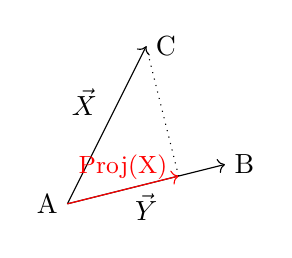
\begin{tikzpicture}
         \coordinate (A) at (0, 0); 
         \coordinate (B) at (2, 0.5);
         \coordinate (C) at (1, 2);
         \coordinate (newB) at (1.4117647059, 0.3529411765);
         \coordinate (dotBC) at (2, 1);
         \node[left] (_) at (A){A};
         \node[right] (_) at (B){B};
         \node[right] (_) at (C){C};
         \draw[->] (A) -- (B);
         \node[above left] (...) at ($(A)!0.5!(C)$) {$\vec{X}$};
         \node[below] (...) at ($(A)!0.5!(B)$) {$\vec{Y}$};
         \draw[->] (A) -- (C);
         \draw[->, red, thin] (A) -- (newB);
         \draw[dotted] (C) -- (newB);
         \node[above, red] (_) at ($(A)!0.5!(newB)$){\small Proj(X)};
      \end{tikzpicture} 
   \end{center}
\end{intuition}
\begin{prop}
    Produit scalaire respectes ces propriétés:
    \begin{enumerate}
        \item bilinaiarité $\quad \lambda \in \R$
            \begin{enumerate}
                \item $(X + Y) \cdot Z = X \cdot Z + Y \cdot Z$
                \item $(\lambda X) \cdot Z = \lambda (X \cdot Z)$
                \item $Z \cdot (X + Y) = Z \cdot X + Z \cdot Y$ 
                \item $Z \cdot (\lambda X) = \lambda (Z \cdot X)$
            \end{enumerate}
        \item symétrie $X \cdot Y = Y \cdot X$
        \item défini positif:  $X \cdot X \ge 0$ et $X \cdot X = 0 \iff X = 0_d$
    \end{enumerate}
\end{prop}
\begin{prop}
    \underline{Cauchy-Schwarz}:\\ 
    \[
        |X \cdot Y| \le (X \cdot X)^{\frac{1}{2}}(Y \cdot Y)^{\frac{1}{2}}
    \] 
\end{prop}
\begin{definition}\label{def:norm_eucl}
    La \textbf{norme euclidienne} d'un vecteur $X$ est noté:
   \[
       \|X\| = \left(\sum_{n=1}^{d} x_i^2\right)^{\frac{1}{2}} = \sqrt{x_1^2 + \ldots + x_d^2} = (X \cdot X)^{\frac{1}{2}}
   \] 
   souvent noté $\|X\|_2$
\end{definition}
\begin{intuition}
   Par le théorème de Pythogore, c'est une longeur de ce vecteur. 
\end{intuition}
\begin{prop}
    La norme suit ces propriétés:
   \begin{enumerate}
       \item $\|\lambda X\| = |\lambda|\|X\| \, X \in \R^d, \, \lambda \in \R$
       \item $\|X + Y\| \le \|X\| + \|Y\| \text{ (inégalité triangulaire)}$
       \item $\|X\| \ge 0$ et $\|X\| = 0 \iff X = 0_d$
   \end{enumerate}
\end{prop}
\begin{explanation}
    de (2)
    \begin{align*}
        \|X + Y\|^2 &= (X + Y)\cdot(X + Y) = X \cdot (X + Y) + Y \cdot (X + Y) = X \cdot X + X \cdot Y + Y \cdot X + Y \cdot Y\\
                    &= \|X\|^2 + 2X \cdot Y + \|Y\|^2 \le \|X\|^2 + 2\|X\| \|Y\| + \|Y\|^2 = (\|X\| + \|Y\|)^2
    \end{align*}
\end{explanation}
\begin{definition}
    Une \underline{norme} sur $\R^d$ est une application  $N: \: \R^d \to \R$ tell que:
    \begin{enumerate}
        \item $N(\lambda X) = |\lambda|N(X)$
        \item  $N(X + Y) \le N(X) + N(Y)$
        \item $N(X) \ge 0$ et $N(X) = 0 \iff X = 0_d$
    \end{enumerate}
\end{definition}
\begin{eg}
   \begin{align*}
       &\|X\|_1 = \sum_{n=1}^{d} |x_i|\\
       &\|X\|_{\infty} = \underset{1\le i \le n}{max} |x_i|
   \end{align*} 
\end{eg}
\section{Éspace $\C^d$}
\begin{definition}
    \[
        \C^d = \{ X = (x_1, \ldots, x_d): \: x_i \in \C\}
    \] 
    \begin{align*}
    &z \in \C \quad \overline{z} = a - ib \quad \overline{z}z = a^2 + b^2 \quad |z| = \sqrt{\overline{z}z} = \sqrt{a^2 + b^2}  \\
    &z = a + ib \qquad a = Re\,z,\,b = Im\,z\\
    &Re\,X = (Re\,x_1, \ldots, Re\,x_d) \in \R^d\\
    &Im\,X = (Im\,x_1, \ldots, Im\,x_d) \in \R^d\\
    &\underset{\in \C^d}{X} = \underset{\in \R^d}{Re\,X} + i\underset{\in \R^d}{\:Im\,X}\\
    \end{align*}
    $\C^d$ est un espace vécrotiel sur  $\C$ (même formules avec $\lambda \in \C$ corps des scalaires)
\end{definition}
\begin{definition}
    \underline{Produit scalaire:}
    \[
        (X|Y) = \sum_{n=1}^{d} \overline{x_i}y_i \in \C
    \] 
\end{definition}
\begin{prop}
   . 
   \begin{enumerate}
       \item $(X|Y)$ est "linéaire par rapport à Y"
           \begin{itemize}
               \item $(Z|X + Y) = (Z|X) + (Z|Y)$
               \item $(Z|\lambda X) = \lambda(Z|X) \quad \lambda \in \C$
               \item  $(Z|\lambda X + \mu Y) = \lambda(Z|X) + \mu(Z|Y)$
               \item  $(X + Y|Z) = (X|Z) + (Y|Z)$
               \item $(\lambda X|Z) = \overline{\lambda}(X|Z) \quad \lambda \in \C$
               \item $(\lambda X + \mu Y|Z) = \overline{\lambda}(X|Z) + \mu(Y|Z)$
           \end{itemize}
       \item $(Y|X) = \overline{(X|Y)}$
       \item $(X|X) = \sum_{n=1}^{d} \overline{x_i}x_i = \sum_{n=1}^{d} |x_i|^2$\\
           $(X|X) \ge 0$ et $(X|X) = 0 \iff X = 0_d$
   \end{enumerate}
\end{prop}
\begin{explanation}
    On a Cauchy-Schwarz:
    \begin{align*}
        (X|Y) \le (X|X)^{\frac{1}{2}}(Y|Y)^{\frac{1}{2}}
    \end{align*}
    même preuve qu'avant
\end{explanation}
On pose:
\begin{align*}
    \|X\| & \text{(ou }\|X\|_2\text{)}\\
          &= (X|X)^{\frac{1}{2}} = \left( \sum_{n=1}^{d} |x_i|^2 \right)^2
\end{align*}
norme hibertienne
\[
    \underset{\in \C^d}{\|X\|^2} = \underset{\in \R^d}{\|Re\,X\|^2} + i\underset{\in \R^d}{\:\|Im\,X\|^2}\\
\] 
\begin{lemma}
   \begin{align*}
       \|X\| = \underset{\|Y\|\le 1}{sup|(X|Y)|}
   \end{align*} 
\end{lemma}
\begin{explanation}
    $|(X|Y)| \le \|X\|\|Y\| \le \|X\|$ si $\|Y\| \le 1$
    \[
    \underset{\|Y\|\le 1}{sup|(X|Y)|}
    \] 
    \underline{Autre sens:} 
    \begin{align*}
        &X \neq 0 \quad Y =  \frac{X}{\|X\|} = \lambda X \quad \lambda = \frac{1}{\|X\|}\\
        &\|Y\| = |\lambda|\|X\| = \frac{1}{\|X\|}\|X\| = 1\\
        &(X|Y) = (X|\frac{X}{\|X\|}) = \frac{1}{\|X\|}(X|X) = \|X\|\\
        &sup \{|(X|Y)|: \, \|Y\| \le  1\}\\
        &\|X\| \le sup \{|(X|Y)|: \, \|Y\|\le 1\} \quad \text{(prendre }Y = \frac{X}{\|X\|}\text{)}
    \end{align*}

\end{explanation}
\underline{Autres normes sur $\C^d$}
\begin{itemize}
    \item $\|X\|_1 = \sum_{n=1}^{d} |x_i| \quad X \in \C^d$
    \item $\|X\|_{\infty} = \underset{1\le i \le d}{sup} |x_i|$
\end{itemize}
\section{Distance sur $\R^d$}
On oublie norme et produit scalaire. On introduit la distance
\begin{definition}\label{def:distance} La distance
    \[
        d(X, Y) = \|X - Y\| 
    \] 
\end{definition}
\begin{definition} La distance euclidienne
    \[
        d(X, Y) = \|X - Y\| = \sqrt{\sum_{n=1}^{d} (x_i - y_i)^2} 
    \] 
\end{definition}
\begin{prop}
    \begin{align*}
        d: \R^d &\longrightarrow \R \\
        (X, Y) &\longmapsto d((X, Y)) 
    .\end{align*}
    \begin{enumerate}
        \item $d(X, Y) = d(Y, X)$ (symétrie)
        \item $d(X, Y) \le d(X, Z) + d(Z, Y)$ (inég. triangulaire) $\forall X, Y, Z$ 
        \item $d(X, Y) \ge 0 \quad \forall X, Y$ et $d(X, Y) = 0 \iff X = Y$ 
    \end{enumerate}
\end{prop}
\begin{eg} Distances
   \begin{enumerate}
       \item $d_2(X, Y) = \|X - Y\|_2$ (distance euclidienne sur $\R^d$)
       \item $d_1(X, Y) = \|X - Y\|_1$\\
           $d_{\infty}(X, Y) = \|X - Y\|_{\infty}$
       \item distance logarithmique sur $\R_+$:  $d(a, b) = |b - a|$
           \[
               \log_{10}(a) = \frac{\log(a)}{\log(10)}
           \] 
           $x, y \in ]0, +\infty[$\\ 
           $d_{\log}(x, y) = |\log_{10}(\frac{y}{x})|$ \\
           $i$ est une distance sur  $]0, +\infty[$\\
           $d_{\log}(100, 110) = \log_{10}(1,1)$
       \item distance SNCF
           \begin{center}
               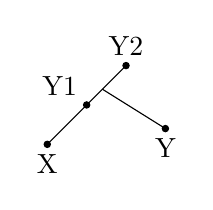
\begin{tikzpicture}
                  \coordinate (X) at (0, 0); 
                  \coordinate (Y) at (1.5, 0.2);
                  \coordinate (Y2) at (1, 1);
                  \coordinate (Y1) at ($(X)!0.5!(Y2)$);
                  \draw (X)--(Y2);
                  \draw (Y)--($(X)!0.7!(Y2)$);
                  \draw[fill=black] (X) circle (0.4mm);
                  \draw[fill=black] (Y) circle (0.4mm);
                  \draw[fill=black] (Y2) circle (0.4mm);
                  \draw[fill=black] (Y1) circle (0.4mm);
                  \node[below] (_) at (X){X};
                  \node[below] (_) at (Y){Y};
                  \node[above left] (_) at (Y1){Y1};
                  \node[above] (_) at (Y2){Y2};
               \end{tikzpicture}
               
           \end{center}
           $d(X, Y)$ distance usuelle dans  $\R^2$
           on pose:
            \begin{align*}
               \delta(X, Y) = \begin{cases}
                   d(X, Y) \text{ si } X, 0, Y \text{ alignés}\\
                   d(X, 0) + d(0, Y) \text{ sinon }
               \end{cases}
           \end{align*}
   \end{enumerate}
\end{eg}
\chapter{Éspaces métriques}
\begin{definition}
    $E$ muni d'une application de distance $d$ (voir Definition \ref{def:distance}) se note  $(E, d)$: \underline{espace métrique}
\end{definition}
\begin{remark}
   si $d_1 \neq d_2$ $(E, d_1)$ n'a rien à faire avec  $(E, d_2)$ 
\end{remark}
\begin{remark}
    Retenir la version suivante de l'inégalité triangulaire:
    \[
        |d(x, z) - d(y, z)| \le d(x, y)
    \] 
\end{remark}
\begin{remark}
    \underline{Distance induite:}\\
    Si $(E, d)$ espace métrique et  $U \subset E$. Je peux restreidnre $d$ à  $U \times U$:  $(U, d)$ est aussi un éspace metrique.
\end{remark}
\section{Boules dans un espace métrique}
\begin{definition}
    $(E, d)$ espace métrique. Soit  $x_0 \in E$ et $r \ge  0$
    \begin{enumerate}
        \item $B(x_0, r) = \{ x \in E: d(x_0, x) < r$ \} boule ouverte de centre $x_0$, de rayon $r$
        \item $B_f(x_0, r) = \{ x \in E: d(x_0, x) \le  r$\} boule fermée de centre $x_0$, de rayon $r$
    \end{enumerate}
\end{definition}
\begin{figure}
    \centering
    \begin{subfigure}{0.45\textwidth}
        \centering
        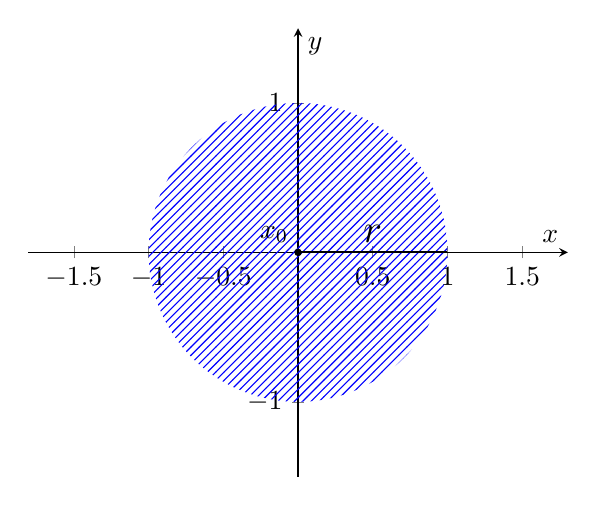
\begin{tikzpicture}
            \begin{axis}[
                axis equal, % Ensures the circle appears round
                axis lines=middle,
                xlabel={$x$},
                ylabel={$y$},
                xmin=-1.5, xmax=1.5,
                ymin=-1.5, ymax=1.5
                ]
                % Plot a circle with radius 1
                \addplot [
                    domain=0:360,       % Angle range
                    samples=200,        % Smoothness
                    fill=none,          % No solid fill color
                    pattern=north east lines, % Hatch pattern
                    pattern color=blue,
                    draw=none           % No outline
                    ] ({cos(x)}, {sin(x)}); 
                \node[above left] (_) at (0, 0){$x_0$};
                \draw[fill=black] (0, 0) circle (0.4mm);
                \draw[thick] (0,0)--(1,0);
                \node[above] (r) at ($(0,0)!0.5!(1,0)$){\Large$r$};
            \end{axis}
        \end{tikzpicture}
        \caption{boules ouverte (i.e $d(x_0, x) < r$)}
    \end{subfigure}
    \hfill
    \centering
    \begin{subfigure}{0.45\textwidth}
        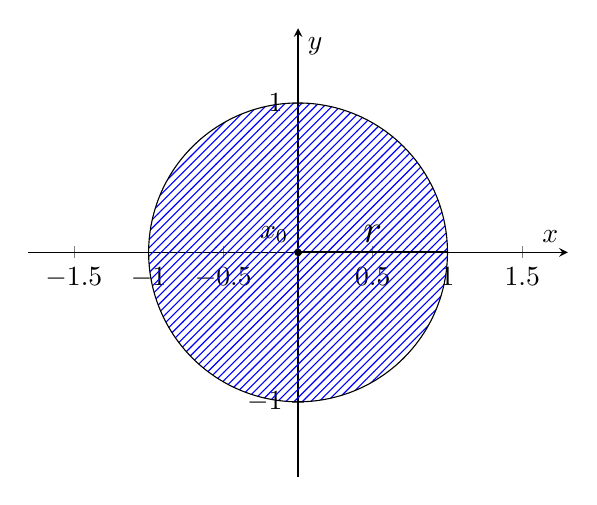
\begin{tikzpicture}
            \begin{axis}[
                axis equal, % Ensures the circle appears round
                axis lines=middle,
                xlabel={$x$},
                ylabel={$y$},
                xmin=-1.5, xmax=1.5,
                ymin=-1.5, ymax=1.5
                ]
                % Plot a circle with radius 1
                \addplot [
                    domain=0:360,       % Angle range
                    samples=200,        % Smoothness
                    fill=none,          % No solid fill color
                    pattern=north east lines, % Hatch pattern
                    pattern color=blue,
                    ] ({cos(x)}, {sin(x)}); 
                \node[above left] (_) at (0, 0){$x_0$};
                \draw[fill=black] (0, 0) circle (0.4mm);
                \draw[thick] (0,0)--(1,0);
                \node[above] (r) at ($(0,0)!0.5!(1,0)$){\Large$r$};
            \end{axis}
        \end{tikzpicture}
        \caption{boules fermée (i.e $d(x_0, x) \le r$)}
    \end{subfigure}
\end{figure}
\begin{lemma}.
   \begin{enumerate}
       \item $B(x_0, 0) = \O$ (car impossible d'avoir des points qui en distance sont strictement plus petit que 0)
       \item $B_f(x_0, 0) = \{x_0\}$
       \item $B(x_0, r_1) \subset B_f(x_0, r_1) \subset B(x_0, r_2)$ si $r_1 < r_2$
       \item $B(x_1, r_1) \subset B(x_0, r)$ si  $d(x_0, x_1) + r_1 \le r$
   \end{enumerate} 
   pic 5
\end{lemma}
\begin{explanation}
   Je suppose que $d(x_0, x_1) \le r$\\ 
   Soit $x \in B(x_1, r_1)$ donc $d(x_1, x) < r_1$ à montrer: $x \in B(x_0, r)$ (i.e $d(x_0, x) < r$?)\\
   L'inégalité triangulaire me dit:
   \begin{align*}
       d(x_0, x) &\le d(x_0, x_1) + d(x_1, x)\\
                 &< d(x_0, x_1) + r_1 \le r\\
                 &\implies x \in B(x_0, r)
   \end{align*}
\end{explanation}

\section{Bases orthonormales}
Soit $(E, \scalair{,})$ un espace euclidien et  $F \subset E$ un sous-espace vectoriel ($dim(F) < \infty$) car $dim(E) < \infty$.
\begin{note}
    \[
        F^{\perp} := \{x \in E \mid \scalair{X, Z} = 0 \, \forall z \in F\} 
    \] 
    l'orthogonale de $F$.
\end{note}
\begin{theorem}
    On a $E = F \oplus F^{\perp}$.\\
    En particulier,  $dim(F^{\perp}) = dim(E) - dim(F)$ et  $F = (F^{\perp})^{\perp}$
\end{theorem}
\begin{preuve}
   On doit montrer que:
   \begin{enumerate}
       \item $F \cap F^{\perp} = \O$
       \item $E = F + F^{\perp}$ i.e  $\forall x \in E, \exists x' \in F, \, x'' \in F^{\perp}$ tq $x = x' + x''$ 
   \end{enumerate}
   \begin{enumerate}
       \item Soit $x \in F \cap F^{\perp}$\\
       $\implies$ $\scalair{X, Z} = 0 \, \forall Z \in F$ car $x \in F \implies \scalair{X, X} = 0 \implies x = 0 (\scalair{,} \text{ est définie})$ 
        \item Soit $x \in E$. Considérons  $f_x \in E^{*}$, i.e  $f_x: E \to \R, y \mapsto \scalair{x, y}$ et $f := f_{x|F}: F \to \R \implies f \in E^{*}$
            Lemme de Riesz $\implies$ $\exists! x' \in F$ tq $f = f_{x'}: F \to \R, z \mapsto \scalair{x', z}$\\
            $\implies f_{x}(z) = f_{x'}(z) = f(z)\, \forall z \in F$ (Attention: pas l'égalité pour tout $z$ dans  $E$)\\
            Posons $x'' := x - x'$, i.e  $x = x' + x'' \in F$. Montrons  $x'' \in  F^{\perp}$.\\
            Si $z \in F$,  $\scalair{x'', z} = \scalair{x - x', z} = \scalair{x, z} - \scalair{x', z} = 0$. Donc $x'' \in F^{\perp}$ et  $E = F \oplus F^{\perp}$ ($dim(E) = dim(F) + dim(F^{\perp})$) \\
            $F \subseteq (F^{\perp})^{\perp}$ car $\scalair{x, z} = 0 \, \forall x \in F \, \forall z \in F^{\perp}$
            \[
                dim(F) = dim(E) - dim(F^{\perp})
            \] 
            car $E = G \oplus G^{\perp}$, donc  $dim(G) = dim(E) - dim(G^{\perp})$ pour  $G = F^{\perp}, \, dim(F^{\perp}) = dim(G)$
   \end{enumerate}
\end{preuve}
\begin{definition}
    Soit $E$ un espace vectoriel muni d'un produit scalaire  $\scalair{,}$
     \begin{itemize}
         \item Une famille $(v_i)_{i \ge 0}$ de vecteurs de $E$ est dite \underline{orthogonale} si pour $i \neq j$ on a $\scalair{v_i, v_j} = 0$ i.e  $v_i \perp v_j$
         \item Une famille orthonormale de  $E$ est une famille orthogonale  $(v_i)_{i \ge  0}$ tq de plus $\|v_i\| = 1$ pour  $i \ge 0$
    \end{itemize}
\end{definition}
\begin{eg}
   \begin{enumerate}
       \item $E = \R^{n}$ muni du produit scalaire canonique. La base canonique $(e_1, \ldots, e_n)$ est orthogonale car 
           \[
           \scalair{e_i, e_j} = \begin{cases}
               1 \text{ si } i = j\\
               0 \text{ si } i \neq j
           \end{cases}
           \] 
       \item Dans $E = \mathcal{C}^{0}([-1, 1], \R)$ muni de $\scalair{f,g} = \int_{-1}^{1} f(t)g(t)\,d{t}$. La famille $(\cos(t), \sin(t))$ est orthogonale. La famille $(1, t^2)$ n'est pas orthogonale:
            \[
                \scalair{1, t^2} = \int_{-1}^{1} 1 t^2 \, d{t} = \frac{2}{3} \neq  0 
           \] 
   \end{enumerate} 
\end{eg}
\begin{prop}
    Une famille orthogonale constituée de vecteurs \underline{non-nuls} est libre. En particulier, une famille orthonormale est libre. 
\end{prop}
\begin{preuve}
    Suppososns $(v_1, \ldots, v_n)$ orthogonale avec $v_i \neq 0 \, \forall i = 1, \ldots, n$\\
    si $\sum_{j=1}^{n} \underset{\in \R}{\alpha_iv_i} = 0$, alors  
    \[
        \forall i \in \{1, \ldots, n\} 0 = \scalair{v_i, \sum_{j=1}^{n} \alpha_jv_j} = \sum_{j=1}^{n}\alpha_j \scalair{v_i, v_j} = \alpha_i \underset{\neq 0}{\|v_i\|^2}
    \] 
    Donc $\alpha_i = 0 \, \forall i = 1, \ldots, n$.\\
    Si $(v_1, \ldots, v_n)$ est orthonormale, alors $\|v_i\| = 1$. Donc  $v_i \neq 0, \, \forall i = 1, \ldots, n$.
\end{preuve}
\begin{intuition}
   Les vecteurs orthogonales (perpendiculaires) ne sont jamais dans l'un l'autre (i.e $e_i = \lambda e_j$ n'est pas possible) si les vecteurs sont liés, soit l'angle est $< 90º$ (donc les vecteurs ne sont pas orthogonales, absurd), (ils sont dans l'un l'autre, ils ne sont pas orthogonales, absurd). Donc ils sont bien libres.
\end{intuition}
\begin{definition}
    $(E, \scalair{,})$ espace euclidien. Une famille  $B = (e_1, \ldots, e_n)$ est une base orthonormale (où BON) si elle est une base et famille orthonormale.
\end{definition}
\begin{theorem}
    $(E, \scalair{,})$ espace euclidien. Alors, il admet une BON.
\end{theorem}
\begin{preuve}
   Soit $n := dim(E)$. Soit  $(e_1, \ldots, e_p)$ une famille orthogonale (du point de vue du cardinal $p$) tq  $e_i \neq 0 \, \forall i = 1, \ldots, p$.\\
Supposons par l'absurde que $p < n$. Posons  $F = Vect(e_1, \ldots, e_p)$. Alors, $E = F \oplus F^{\perp}$ et  $dim(F) \le p < n$. Donc $F^{\perp} \neq  \{0\}$. Soit $x \in F^{\perp}, \, x \neq 0$. Alors, $(e_1, \ldots, e_p, x)$ est orthogonale de cardinale $> p$. Donc,  $p = n$ et  $(e_1, \ldots, e_n)$ est une base de $E$. Pour avoir une famille orthonormale  $(e_1', \ldots, e_n')$ il suffit de prendre $e_i' = \frac{1}{\|e_i\|}e_i \, \forall i = \{1, \ldots, n\}$.
\end{preuve}
\begin{prop}
    Soit $(E, \scalar{}{})$ un espace euclidien et soit  $(e_1, \ldots, e_n)$ une BON de $E$. Si  $x \in E$, on a:
   \[
       x = \sum_{i=1}^{n} \scalar{x}{e_i}e_i
   \] 
Autrement dit, le réél $\scalar{x}{e_i}$ est la  $i^{\text{ème}}$ coordonnée de $x$ dans la base  $(e_1, \ldots, e_n)$.
\end{prop}
\begin{intuition}
    L'orthonormalité de la base nous simplifie la vie. Mais avant, petite introduction. Soit un e.v $E = \R^2$ et la base $(e_1, e_2) = (\begin{pmatrix} 1 \\ 0 \end{pmatrix}, \begin{pmatrix} 0\\ 1 \end{pmatrix})$. Soit un vecteur $\vec{v} = (2, 3)$ :
    \begin{center}
        \begin{tikzpicture}
            \begin{axis}[
                scale=1,
                axis lines=middle,        % Draw axes in the middle
                xmin=-2, xmax=4,          % X-axis range
                ymin=-2, ymax=4,          % Y-axis range
                xlabel={$x$},             % Label for X-axis
                ylabel={$y$},             % Label for Y-axis
                xtick={-2,-1,0,1,2,3,4},% X-axis ticks
                ytick={-2,-1,0,1,2,3,4},% Y-axis ticks
                ]
            \draw[color=red, ->, thick] (0, 0) -- node[below]{$e_1$}(1, 0);
            \draw[color=blue, ->, thick] (0, 0) -- node[left]{$e_2$}(0, 1);
            \draw[color=green, ->] (0, 0) --node[above]{$\vec{v}$} (2, 3);

            \draw[color=gray, ->, thick] (1, 0) -- node[below]{$e_1$}(2, 0);
            \draw[color=gray, ->, thick] (2, 0) -- node[left]{$e_2$}(2, 1);
            \draw[color=gray, ->, thick] (2, 1) -- node[left]{$e_2$}(2, 2);
            \draw[color=gray, ->, thick] (2, 2) -- node[left]{$e_2$}(2, 3);

            \node[right, above] (_) at (2, 3){$(2, 3)$};
        \end{axis} 
        \end{tikzpicture}
    \end{center}
    Donc, on peut écrire $\vec{v} = \vec{(2, 3)} = 2 \cdot \vec{e_1} + 3 \cdot \vec{e_2}$. Les $x$ et  $y$ (les coordonnées de $v$) nous donnes combien de parties de chaque vecteur de bases (le nombre peut être $\in \R$) et prendre leurs sommes, pour obtenir $\vec{v}$. (Le plus simple: combien on doit aller à gauche et en haut).
    \par
    Dans la base orthonormale $\scalair{v, e_i}$ nous donne combien on prend d'un vecteur $e_i$ pour faire le vecteur  $\vec{v}$ et  $\vec{e_i}$ donne la direction. D'où $\scalair{v, e_1}$ équivaut à $2$, et  $\scalair{v, e_2}$ à  $3$, puis: 
   \[
       \vec{v} = \underbrace{\scalair{v, e_1}}_{= 2} \cdot \vec{e_1} + \underbrace{\scalair{v, e_2}}_{= 3} \cdot \vec{e_2}
   \]  
   Habituelement, pour trouver les coordonnées dans une base, on devrait résoudre un système linéaire, tandis qu’une base orthonormale permet de les obtenir en calculant le produit scalaire avec chaque vecteur de la base, ce qui est beaucoup plus simple.
\end{intuition}
\begin{preuve}
    Posons $y := \sum_{i=1}^{n} \scalar{x}{e_i}e_i$ . Alors, 
   \begin{align*}
       &\forall j = 1, \ldots, n,\\
       &\scalar{x - y}{e_j}\\ 
       = &\scalar{x}{e_j} - \scalar{y}{e_j}\\ 
       = &\scalar{x}{e_j} - \scalar{\sum_{i=1}^{n} \scalar{x}{e_i}e_i}{e_j}\\ 
       = &\scalar{x}{e_j} - \underbrace{ \sum_{i=1}^{n} \scalar{x}{e_i} }_{\substack{\text{moved out}\\ \text{like constant}}}\scalar{e_i}{e_j}\\ 
       = &\scalar{x}{e_j}\\ 
       -& \left(\scalar{x}{e_1}\underbrace{ \scalar{e_1}{e_j} }_{= 0} + \ldots + \scalar{x}{e_{j-1}}\underbrace{\scalar{e_{j-1}}{e_j}}_{= 0} + \scalar{x}{e_{j}}\underbrace{ \scalar{e_{j}}{e_j} }_{= 1} + \scalar{x}{e_{j+1}}\underbrace{ \scalar{e_{j+1}}{e_j} }_{= 0} + \ldots + \scalar{x}{e_{n}}\underbrace{ \scalar{e_{n}}{e_j} }_{= 0}\right)\\
        &\text{(} \forall i \neq j, \, \scalar{e_i}{e_j} = 0 \text{ car un produit scalaire des vecteur orthogonaux)}\\ 
        &\text{(} \forall j \, \scalar{e_j}{e_j} = 1 \text{ car un produit scalaire de même vecteur)}\\
       = &\scalar{x}{e_j} - \scalar{x}{e_j}\underset{= 1}{\scalar{e_j}{e_j}} = 0
   \end{align*}
   Donc, $x - y \in Vect(e_1, \ldots, e_n)^{\perp} = E^{\perp} = \{0\}$. Donc $x = y$
\end{preuve}
\begin{corollary}
    $\forall x \in E, \, \|x\|^2 = \sum_{i=1}^{n} \scalar{x}{e_i}^2$ 
\end{corollary}
\begin{preuve}
    Si $x = \sum_{i=1}^{n} \scalar{x}{e_i}e_i = \sum_{i=1}^{n} x_ie_i$ donc
    \[
        \|x\|^2 = \scalar{\sum_{i=1}^{n} x_ie_i}{\sum_{j=1}^{n} x_je_j} = \sum_{i,j=1}^{n} x_ix_j\scalar{e_i}{e_j} = \sum_{i=1}^{n} x_i^2
    \] 
\end{preuve}
\section{Matrices et produits scalaires}
\begin{prop} Soient $(E, \scalair{,})$ un espace euclidien et $\epsilon = (e_1, \ldots, e_n)$ une BON. Soient $f \in \mathcal{L}(E, E)$ et $A = (a_{i,j})_{1 \le i,j \le n}$ la matrice représentative de $f$ dans  $\epsilon$, i.e,  $A = Mat_{\epsilon}(f)$ 
    \[
        a_{i,j} = \scalair{f(e_i), e_j} \, \forall i,j = 1, \ldots, n
    \] 
\end{prop}
\begin{preuve}
   $A$ est la matrice dont les colonnes sont les vecteurs  $f(e_j)$ écrits dans la base $\epsilon$:
    \[
        A = (f(e_1) | \ldots | f(e_n))\quad f(e_j) = \begin{pmatrix} a_{1,j}\\ \ldots\\ a_{n, j} \end{pmatrix} 
   \] 
   Car $\forall v \in E, \, v = c_1e_1 + \ldots c_ne_n$ donc $f(v) = c_1f(e_1) + \ldots c_nf(e_n)$ par la linéarité, donc il nous reste à étudier chaque $f(e_j)$
   \begin{align*}
       f(e_j) = a_{1, j}e_1 + \ldots a_{n, j}e_n \implies\\
       \langle f(e_j), e_i \rangle = \left\langle \sum_{k=1}^n a_{k,j} e_k, e_i \right\rangle = \sum_{k=1}^{n} a_{k,j}\scalar{e_k}{e_i} = a_{k, j}
   \end{align*}
   car $\scalar{e_k}{e_j} = \begin{cases}
       0 \text{ si } k \neq j\\
       1 \text{ si } k = j
   \end{cases}$
   Donc:
   \[
       a_{i, j} = \scalair{f(e_j), e_i}
   \] 
\end{preuve}


La matrice d'un produit vectoriel est très utile dans l'algèbre linéaire. Avant donner une definition:
\par
Soit $E$ un espace vectoriel de dimension finie  $n$, un espace  $K$ et une forme bilinéaire  $b: E \times E \longrightarrow K$. Si $\{e_1, \ldots, e_n\}$ est une base de $E$, alors:  $x = \sum_{i=1}^{n} x_ie_i$ et $y = \sum_{j=1}^{n} y_je_j$, alors on a:
\[
b(x, y) = \sum_{i,j = 1}^{n} x_iy_jb(e_i, e_j)
\] 
$b$ est donc détérminé par la conaissance des valeurs  $b(e_i, e_j)$ sur une base.
 \begin{definition}
     On appelle  \textbf{matrice de $b$} dans la base $\{e_i\}$ la matrice:
      \[
          M(b)_{e_i} = \begin{pmatrix} 
              b(e_1, e_1) & b(e_1, e_2) & \ldots & b(e_1, e_n)\\
              b(e_2, e_1) & b(e_2, e_2) & \ldots & b(e_2, e_n)\\
              \ldots & \ldots & \ldots & \ldots\\
              b(e_n, e_1) & \ldots & \ldots & b(e_n, e_n)
          \end{pmatrix} 
     \] 
     Ainsi l'élément de la $\text{i}^{\text{ème}}$ ligne et $\text{j}^{\text{ème}}$ colonne est le coefficient de $x_iy_j$.
\end{definition}
\begin{eg}
   La matrice du produit scalair canonique dans $\R^3$ est:
   \[
       \scalair{X, Y} = x_1y_1 + x_2y_2 + x_3y_3 
   \] 
   \[
       Mat(\scalair{,})_{e_i} = \begin{pmatrix} 
            1 & 0 & 0\\
            0 & 1 & 0\\
            0 & 0 & 1
       \end{pmatrix} 
   \] 
\end{eg}
\begin{prop}\label{prop:prod-scal-par-matrice} produit scalair représenté par une matrice.\par
   Notons:
   \begin{align*}
       \underbrace{A = M(b)_{e_i}}_{\text{matrice de produit scalair}} && \underbrace{X = M(x)_{e_i}}_{\substack{\text{coordonnées de $x$}\\ \text{dans la base  $e_i$}}} && \underbrace{Y = M(y)_{e_i}}_{\substack{\text{coordonnées de $y$}\\ \text{dans la base $e_i$}}} && (x, y \in E)
   \end{align*}
   Alors, on a:
   \[
       b(x, y) = X^{t}AY
   \] 
\end{prop}
\begin{eg}
    Repronnons l'exemple avec $b = \scalair{,}$ le produit scalair canonique dans  $\R^3$. Soit $X = \begin{pmatrix} 1 \\ 2 \\ -1 \end{pmatrix}$ et $Y = \begin{pmatrix} 2 \\ 3 \\ 1 \end{pmatrix} $ dans la base canonique de $\R^3$. Donc:
    \begin{align*}
        \scalair{x, y} = X^{t}AY &= \overbrace{(1, 2, -1)}^{X^{t}} \times \overbrace{\begin{pmatrix} 1 & 0 & 0\\ 0 & 1 & 0\\ 0 & 0 & 1 \end{pmatrix}}^{A} \times \overbrace{ \begin{pmatrix} 2 \\ 3 \\ 1 \end{pmatrix} }^{Y} \\
                                 &= \underbrace{(1, 2, -1)}_{X} \times \underbrace{ \begin{pmatrix} 2 \\ 3\\ 1 \end{pmatrix} }_{A \times Y} \\
                                 &= 1 \cdot 2 + 2 \cdot 3 + (-1) \cdot 1 = 2 + 6 - 1 = 7
    \end{align*}
\end{eg}
\begin{TODO}
   changement de base de la matrice d'une forme bilinéaire 
\end{TODO}

\section{Projections orthogonales}
Soit $(E, \scalair{,})$ un espace euclidien,  $F \subseteq E$ un sous-espace vectoriel. Alors,  $E = F \oplus F^{\perp}$. Donc $\forall x \in E$ s'ecrit 
\[
x = \underset{\in F}{x_F} + \underset{\in F^{\perp}}{x_{F^{\perp}}}
\] 
\begin{definition}
    La \textbf{projection orthogonale} de $E$ dans  $F$ est la projection  $p_F$ de  $E$ sur  $F$ parallèlement  à $F^{\perp}$, i.e
    \begin{align*}
        p_F: E = F \oplus F^{\perp} &\longrightarrow F \\
        x = x_F + x_{F^{\perp}} &\longmapsto p_F(x = x_F + x_{F^{\perp}}) = x_F
    .\end{align*}
\end{definition}
\begin{remark}
   \begin{enumerate}
       \item $p_F$ est linéaire
       \item  $\forall x \in E \, p_{F}(x)$ est complétement caractérisé par la propriété suivante:\\
           Soit $y \in E$, alors
            \[
                y = p_F(x) \iff \left( \underset{\implies y = x_F}{y \in F \text{ et } x - y} \in F^{\perp} \right) 
           \] 
       En particulier $\scalair{p_F(x), x - p_F(x)} \,= 0$. Alors, si $(v_1, \ldots, v_R)$ est une BON de $F$, on a:
            \[
                \forall x \in E, \, p_F(x) = \sum_{i=1}^{k} \scalair{x, v_i}v_i
           \] 
           En effet, il suffit de vérfier que le vecteur $y = \sum_{i=1}^{k} \scalair{x, v_i}v_i$ vérfie:
           \[
               y \in F \text{ et } x - y \in F^{\perp}
           \] 
   \end{enumerate} 
\end{remark}
\begin{figure}[H]
   \centering 
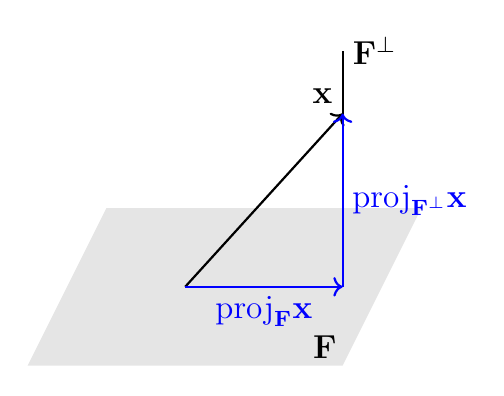
\begin{tikzpicture}

% Draw the plane
\fill[gray!20] (-2,-1) -- (2,-1) -- (3,1) -- (-1,1) -- cycle;

% Draw the vectors
\draw[->, thick, black] (0,0) -- (2,2.2) node[anchor=south east] {\large $\mathbf{x}$};

\node[anchor=north, blue] (_) at ($(0,0)!0.5!(2,0)$) {\large $\text{proj}_\mathbf{F} \mathbf{x}$};
\node[anchor=west, blue] (_) at ($(2,0)!0.5!(2,2.2)$) {\large $\text{proj}_\mathbf{F^{\perp}} \mathbf{x}$};
% Add the labels for w and w perpendicular
\draw[->, thick, blue] (0,0) -- (2,0) ;
\draw[thick, black] (2,0) -- (2,3) node[anchor=west] {\large $\mathbf{F}^\perp$};
\draw[->, thick, blue] (2,0) -- (2,2.2);
\node[anchor=north west] (_) at (1.5, -0.5) {\large $\mathbf{F}$};
% Add the right angle symbol

\end{tikzpicture}
\caption{Projection}
\label{pic:projection}
\end{figure}
\begin{figure}[ht]
    \centering
    \incfig{projection-with-bon}
    \caption{Projection avec BON}
    \label{fig:projection-with-bon}
\end{figure}
\begin{prop}
   Soit $x \in E$. Alors,
   \[
       \|x - p_F(x)\| = inf\{\|x - y\| \mid y \in F\}
   \] 
   i.e $\|x - p_F(x)\|$ est la distance de  $x$ à  $F$.\\
   Voir Figure~\ref{pic:projection}
\end{prop}
\begin{preuve}
   Comme $p_F(x) \in F$ il suffit de prouver que, si  $y \in F$, alors 
   \[
   \|x - p_F(x)\| \le \|x - y\|
   \] 
   Mais, $\underset{(x - p_F(x)) + (p_F(x) - y)}{\|x - y\|^2} = \|x - p_F(x)\|^2 + 2\overbrace{\scalair{\overset{\in F^{\perp}}{x - p_F(x)}, \overset{\in F}{p_F(x) - y}}}{= 0} + \underbrace{\|p_F(x) - y\|^2}_{\ge 0} \ge \|x - p_F(x)\|^2$
\end{preuve}
\begin{theorem}\label{thm:gram-schmidt}Gram-Shmidt\\
    Soit $E$ un espace vectoriel muni d'un produit scalaire  $\scalair{,}$. Soit  $(v_1, \ldots, v_n)$ une famille libre d'élement $\in E$. Alors,  il existe une famille $(w_1, \ldots, w_n)$ orthogonale tq 
    \[
        \forall i = 1, \ldots, n \quad Vect(v_1, \ldots, v_i) = Vect(w_1, \ldots, w_i)
    \] 
    De plus, ce théorème nous donne un procédé de construction d'une base orthonormée à partir d'une base quelconque.
\end{theorem}
\begin{preuve} du Théorème \ref{thm:gram-schmidt}
    Construisons la base orthogonale: $\{w_1, \ldots, w_p\}$. Posons d'abord:
    \[
    \begin{cases}
        w_1 = v_1\\
        w_2 = v_2 + \lambda w_1, \qquad \text{avec } \lambda \text{ tel que } w_1 \perp w_2
    \end{cases}
    \] 
    En imposant cette condition on trouve:
    \[
        0 = \scalair{v_2 + \lambda w_1, w_1} = \scalair{v_2, w_1} + \lambda \|w_1\|^2
    \] 
    Comme $w_1 \neq 0$, on obtient $\lambda = - \frac{\scalair{v_2, w_1}}{\|w_1\|^2}$. On remarque que:
    \[
    \begin{cases}
        v_1 = w_1\\
        v_2 = w_2 - \lambda w_1
    \end{cases}
    \] 
    donc $Vect\{v_1, v_2\} = Vect\{w_1, w_2\}$.
    \par
    Une fois construit $w_2$, on construit $w_3$ en posant:
    \begin{align*}
        &w_3 = v_3 + \mu w_1 + \nu w_2\\
        &\text{avec } \mu \text{ et } \nu \text{ tels que: } w_3 \perp w_1 \text{ et } w_3 \perp w_2
    \end{align*}
    On peut voir $w_3 = v_3 - \lambda' w_1 - \lambda'' w_2 $ comme $w_3 = v_3 - proj_{F_2}v_3$ où $F_i = Vect\{w_1, \ldots, w_i\}$
    \begin{figure}[H]
        \centering
        \incfig{projection-with-bon-thm}
        \caption{Vecteur par projection}
        \label{fig:projection-with-bon-thm}
    \end{figure}
    Ceci donne
    \begin{align*}
        0 &= \scalair{v_3 + \mu w_1 + \nu w_2, w_1} = \scalair{v_3, w_1} + \mu \underset{= \|w_1\|^2}{\scalair{w_1, w_1}} + \nu \underset{= 0}{\scalair{w_2, w_1}}\\
          &= \scalair{v_3, w_1} + \mu \|w_1\|^2 
    \end{align*}
    d'où $\mu = - \frac{\scalair{v_3, w_1}}{\|w_1\|^2}$. De même, en imposant que $w_3 \perp w_2$, on trouve $\nu = - \frac{\scalair{v_3, w_2}}{\|w_2\|^2}$. Comme
    \[
    \begin{cases}
        v_1 = w_1\\
        v_2 = w_2 - \lambda w_1\\
        v_3 = w_3 - \mu w_1 - \nu w_2
    \end{cases}
    \] 
    on voit bien que $Vect\{w_1, w_2, w_3\} = Vect\{v_1, v_2, v_3\}$. C'est-à-dire, $\{w_1, w_2, w_3\}$ est une base orthogonale de l'éspace engendre par $v_1, v_2, v_3$. On voit bien maintenant le procédé de récurrence.
    \par
    Supposons avoir construit $w_1, \ldots, w_{k-1}$ pour $k \le p$. On pose:
    \begin{align*}
        w_k &= v_k + \text{ combinaison linéaire des vecteurs déjà trouvés}\\
            &= v_k + \lambda_1w_1 + \ldots + \lambda_{k-1}w_{k-1}
    \end{align*}
    Les conditions $w_k \perp w_i$ (pour $i \in \{1, \ldots, k-1\}$) sont équivalentes à:
    \[
        \lambda_i = - \frac{\scalair{v_k, w_i}}{\|w_i\|^2}
    \] 
    comme on le vérifie immédiatement. Puisque $v_k = w_k - \lambda_1 - \ldots - \lambda_{k-1}w_{k-1}$, on voit par récurrence que $Vect\{w_1, \ldots, w_k\} = Vect\{v_1, \ldots, v_k\}$ $\iff$ $\{w_1, \ldots, w_k\}$ est une base orthogonale de $Vect\{v_1, \ldots, v_k\}$.
    \par
    Ce qu'il nous rester c'est à la normaliser, i.e  $\forall i \in \{1, \ldots, k\}$ $e_i = \frac{w_i}{\|w_i\|}$, d'où $\{e_1, \ldots, e_k\}$ est une base orthonormale de $F = Vect\{v_1, \ldots, v_k\}$.
\end{preuve}
\begin{prop} Pour comprendre cette proposition, je vous conseil de lire la section \ref{sec:isometrie-et-adjoints}
    \par
   Toute projection orthogonale est autoadjoint, i.e si $p$ est une projection orthogonale, donc:
   \[
   p^* = p
   \] 
   En notation matricielle: soit $A$ une matrice de la projection  $p$, donc:
    \[
   A^T = A
   \] 
\end{prop}

\section{Isométries et Adjoints}\label{sec:isometrie-et-adjoints}
\subsection{Isométries}
\begin{definition}
    Une \textbf{isométrie} de $E$ (ou \textbf{transformation orthogonale}) est un endomorphisme  $f \in \mathcal{L}(E) := \mathcal{L}(E, E)$ préservant le produit vectoriel, i.e:
     \[
         \scalair{f(x), f(y)} = \scalair{x, y} \quad \forall x, y \in E
    \] 
\end{definition}
\begin{definition}
    Soient $x, y \in E$ deux vecteurs non nuls. On a, d'après l'inégalité de Cauchy-Schwarz (voir lemma \ref{lemma:inegalite-cauchy-schwarz}):
    \[
        \frac{| \scalair{x, y} |}{\|x\| \cdot \|y\|} \le 1
    \] 
    Alors, il existe un et un seul $\theta \in [0, \pi]$ tel que:
     \begin{equation}
        \cos \theta = \frac{ \scalair{x, y}}{\|x\| \cdot \|y\|} 
    \end{equation}
    $\theta$ est dit \textbf{angle} (non-orienté) entre les vecteurs  $x$ et  $y$.
\end{definition}
\begin{prop}\label{prop:isometrie-reserve-norme}
   Si  $f$ est une isométrie de  $E$, donc, on a:
   \[
   \|f(x)\| = \|x\| \quad \forall x \in E
   \] 
\end{prop}
\begin{preuve}
   Supposons que $f$ est une isométrie de  $E$. Soit  $x, y \in E$. Par définition:  $\scalair{f(x), f(y)} = \scalair{x, y}$, donc, posons $y := x$, alors, on a:
   \begin{align*}
       &\underbrace{\scalair{f(x), f(x)}}_{\|f(x)\|^2} = \underbrace{\scalair{x, x}}_{\|x\|^2}\\
       \iff &\|f(x)\|^2 = \|x\|^2\\
       \iff &\|f(x)\| = \|x\|
   \end{align*}
\end{preuve}
\begin{prop}\label{prop:isometrie-bijective}
   Soit $f$ une isométrie dans  $E$, alors:
   \begin{enumerate}
       \item $f$ est bijective 
       \item  $f$ présérve la distance euclidienne et les angles
   \end{enumerate}
\end{prop}
\begin{preuve}
   Soit $f$ une isométrie dans  $E$ et deux vecteurs  $u, v \in E$ 
   \begin{enumerate}
       \item  
           \begin{align*}
               \|f(u) - f(v)\| = \sqrt{\scalair{f(u), f(v)}} = \sqrt{\scalair{u, v}} = \|u - v\| 
           \end{align*}
       \item Soit $\theta_1$ angle entre  $f(u)$ et  $f(v)$ et $\theta_2$ angle entre  $u$ et  $v$, donc:
            \[
                \cos \theta_1 := \frac{\scalair{f(u), f(v)}}{\|f(u)\| \cdot \|f(v)\|}
           \] 
           \[
                \cos \theta_2 := \frac{\scalair{u, v}}{\|u\| \cdot \|v\|}
           \] 
           Par définition, $\scalair{f(u), f(v)} = \scalair{u, v}$, d'après proposition \ref{prop:isometrie-reserve-norme},  $\forall x, \|f(x)\| = \|x\|$, donc:
           \[
                \cos \theta_1 := \frac{\scalair{f(u), f(v)}}{\|f(u)\| \cdot \|f(v)\|} = \frac{\scalair{u, v}}{\|u\| \cdot \|v\|} = \cos \theta_2
           \] 
   \end{enumerate}
\end{preuve}
\begin{definition}
    Soit $F$ un sous-espace vectoriel de  $E$, donc  $E = F \oplus F^{\perp}$ d'où  $\forall v \in E, \exists v_1 \in F, v_2 \in F^{\perp}$ tel que $v = v_1 + v_2$. On pose:
    \[
    s_F(v) = v_1 - v_2
    \] 
    et on appelle $s_F$ une symétrie orthogonale d'axe F.
\end{definition}
\begin{figure}[H]
    \centering
    \incfig{symetrie-orthogonale-axe-f}
    \caption{Symétrie orthogonale d'axe $F$}
    \label{fig:symetrie-orthogonale-axe-f}
\end{figure}
\begin{prop}
   La symétrie orthogonale est une isométrie. 
\end{prop}
\begin{proof}
   TODO ou pas besoin 
\end{proof}
\begin{prop}\label{prop:isometrie-ssi-transforme-bon-en-bon}
   $f$ est une isométrie si et seulement si elle transforme toute base orthonormée en une base orthonormée. 
\end{prop}
\begin{preuve}
    Soit $f$ une isométrie, alors elle transforme toute base en une base car  $f$ est bijective par la prop. \ref{prop:isometrie-bijective}. 
    \begin{itemize}
        \item ($\implies$) Soit $\{e_i\}$ une base orthonormée, alors, on a:
             \[
                 \scalair{f(e_i), f(e_j)} = \scalair{e_i, e_j} = \delta_{i,j}
            \] 
            Donc, $\{f(e_i)\}$ est une base orthonormée.
        \item ($\impliedby$) Supposons, qu'il existe une base orthonormée $\{e_i\}$ telle que  $\{f(e_i)\}$ est aussi une base orthonormée. De plus, soit  $x = x_1e_1 + \ldots x_ne_n$ et $y = y_1e_1 + \ldots + y_ne_n$ avec $x_i, y_i \in \R$
            \par
            Comme $\{e_i\}$ est orthonormée, alors on a:
             \[
                 \scalair{x, y} = x_1y_1 + \ldots + x_ny_n = \sum_{i=1}^{n} x_iy_i
            \] 
            D'autre part:
            \begin{align*}
                \scalair{f(x), f(y)} &= \scalair{\sum_{i=1}^{n} x_if(e_i), \sum_{i=1}^{n} y_if(e_i)} = \sum_{i,j = 1}^{n} x_iy_j\scalair{f(e_i), f(e_j)}\\
                                     &= \sum_{i,j=1}^{n} x_iy_j\scalair{e_i, e_j} \underset{\text{car } f \text{ isométrie}}{=} = \sum_{i=1}^{n} x_iy_i \underset{\text{car } \{e_i\} \text{ orthonormée}} = \scalair{x, y}
            \end{align*}
            Donc $f$ est une isométrie.
    \end{itemize}
\end{preuve}
\begin{prop}\label{prop:isometrie-ata-eg-i}
    Si $\{e_i\}$ est une base orthonormée, $f$ une isométrie et  $A = M(f)_{e_i}$, alors  $A^{T}A = I = AA^{T}$.
\end{prop}
\begin{preuve}
    Pour prouver cela, on va utiliser la proposition \ref{prop:prod-scal-par-matrice}. 
    \par
    Par définition de l'isométrie, on a:
    \begin{align*}
        &\scalair{f(x), f(y)} = \scalair{x, y} \quad \forall x, y \in E\\
        \iff &\underbrace{ (AX)^{T}(AY) }_{\scalair{f(x), f(y)}} = X^TA^TAY = \underbrace{X^TY}_{\scalair{x, y}}\\
        \iff &A^TA = I
    \end{align*}
\end{preuve}
\begin{prop}
   Si $A$ est une matrice de l'isométrie dans une base orthonormée, alors  $det(A) = \pm 1$ 
\end{prop}
\begin{preuve}
    Par la proposition \ref{prop:isometrie-ata-eg-i}, on a: $A^TA = I$, d'où:
     \begin{align*}
         det(A^TA) = det(I) = 1 \implies& det(A)^2 = 1 \quad \text{ (car }  det(A^T) = det(A) \text{)}\\
                                \implies& det(A) = \pm 1
    \end{align*}
\end{preuve}
\begin{intuition}
   Une isométrie fait une rotation ou une réflexion, elle concerve les ditance, donc l'air (ou volume) d'une figure qui est construit par la base de cette transfomation est égale à $1$. 
\end{intuition}

\subsection{Endomorphisme adjoint}
\begin{prop}
   Soit $E$ un espace euclidien et  $f \in End(E)$. Il existe un et un seul endomorphisme  $f^* \in E$ tel que
   \[
       \scalair{f(x), y} = \scalair{x, f^*(y)}, \quad \forall x, y \in E
   \] 
   $f^*$ est dit  \textbf{adjoint} de $f$.
   \par
   Si  $\{e_i\}$ est une base orthonormée et  $A = M(f)_{e_i}$, alors la matrice $A^* = M(f^*)_{e_i}$ est la transposée de $A$, i.e  $A^* = A^T$
\end{prop}
\begin{preuve}
    Encore, pour la preuve, on va utiliser la proposition \ref{prop:prod-scal-par-matrice} qui est très utile, donc je vous conseil maîtriser ce concept.
    \par
    Soit $\{e_i\}$ une base orthonormée de $E$ et notons
     \[
    A = M(f)_{e_i} \quad A^* = M(f^*)_{e_i} \quad X = M(x)_{e_i} \quad Y = M(y)_{e_i}
    \] 
    Comme on est dans une base orthonormée, alors l'énoncé s'ecrit:
    \[
        \underbrace{(AX)^TY}_{\scalair{f(x),y}} = X^TA^TY = \underbrace{X^T(A^*Y)}_{\scalair{x, f^*(y)}} \quad \forall X, Y \in \mathcal{M}_{n, 1}(\R)
    \] 
    ce qui implique que $A^* = A$ et, de plus, démontre l'unicité de tel adjoint.
\end{preuve}


\section{Groupes orthogonaux}
Rappel:
\begin{definition}\label{def:general-linear-group}
    Un groupe linéaire général:
    \[
        GL(n, \R) = \{A \in \mathcal{M}_{n}(\R) \mid det(A) \neq 0\}
    \] 
    est un groupe de toutes transfomrations linéaires (matrices carrées) qui sont invérsibles (car $det(A) \neq 0$).
\end{definition}

\begin{definition} \textbf{Groupe orthogonal}:
    L'ensemble:
    \[
        O(n, \R) := \{A \in \mathcal{M}_{n}(\R) \mid A^TA = I\} = \{A \in \mathcal{M}_{n}(\R) \mid AA^T = I\}
    \] 
    vérifie les propriétés suivantes:
    \begin{enumerate}
        \item si $A, B \in O(n, \R)$, donc $AB \in O(n, \R)$
        \item $I \in O(n, \R)$
        \item si $A \in O(n, \R)$ alors $A^{-1} \in O(n, \R)$
    \end{enumerate}
    En particulier, $O(n, \R)$ est un sous-groupe de $GL(n, \R)$ (groupe des matrices inversibles) (voir la definition \ref{def:general-linear-group}).
\end{definition}
\begin{intuition}
    La signification des matrices orthogonales est claire: elles représentent les matrices des transformations orthogonales (isométrie) dans \textbf{une base orthonormée} (voir defn \ref{def:orthogonal}). 
\end{intuition}
On peut remarquer que si $det(A) = 1$, cette isométrie représente une rotation, de plus, on a la définition suivante:
 \begin{definition}
    L'ensemble des matrices orthogonales directes (i.e telles que $det(A) = 1$)
    \[
    SO(n, \R) = \{A \in O(n, \R) \mid det(A) = 1 \}
    \] 
    est un groupe, dit  \textbf{groupe spécial orthogonal}.
\end{definition}
\begin{eg}
   La matrice
   \[
       A = \frac{1}{3} \begin{pmatrix} 2 & -1 & 2\\ 2 & 2 & -1\\ -1 & 2 & 2 \end{pmatrix} 
   \] 
   est orthogonale. On peut vérifier que $A^TA = I$, ou, il suffit de montrer que  $c_1, c_2, c_3$ est une famille orthonormée, i.e:
   \[
       \|c_i\|^2 = 1 \quad \text{ et } \quad \scalair{c_i, c_j} = 0 \quad \text{ si } i \neq j
   \] 
   On peut interpreter $A$ comme une matrice d'une transformation $f$ dans la base canonique $\{e_i\}$, donc on a bien:  $c_i = f(e_i)$, d'après la proposition \ref{prop:isometrie-ssi-transforme-bon-en-bon} $f$ est orthogonale. De plus, on voit que  $det(A) = +1$. En conséquent,  $f$ est une transformation orthogonale directe.
\end{eg}
\begin{prop}
   La matrice de passage d'une base orthonormée à une base orthonormée est une matrice orthogonale. 
\end{prop}
\begin{preuve}
   Je donne de l'intuition. Matrice de passage transforme une base en autre base, elle passe les vecteurs de la base, alors elle transforme la base de la BON en vecteurs de la base de la BON, donc, d'après la proposition \ref{prop:isometrie-ssi-transforme-bon-en-bon}, cette matrice est orthogonale.
\end{preuve}

\chapter{Déterminants}
Ce chapitre est plutôt un cheatsheet des déterminants car je ne vais pas donner des preuves mais les propriétés utiles, les exemples et de l'intuition.

\begin{definition}
    Soit $A = [a_{i, j}] \in \mathcal{M}_{n}(\R)$ une matrice carée $n \times n$, alors:
    \[
        \operatorname{det}(A) = \sum_{\sigma \in S_n}^{} \operatorname{signe}(\sigma) \cdot \prod_{i=1}^{n} a_{i, \sigma(i)} 
    \] 
    où 
    \begin{itemize}
        \item $S_n$ est un groupe de toute permutation de  $\{1, \ldots, n\}$
        \item $\operatorname{signe}(\sigma)$ est une signe de pérmutation
    \end{itemize}
\end{definition}

Cette définition est très formelle, alors au bout de ce chapitre on va reformuler cette définition. D'abord, on va étudier les propriétés de déterminants:

\section{Propriétés les plus improtants}
\begin{prop} les propriétés de déterminant.
    Pour cette proposition, on note $\det(c_1, \ldots, c_n)$ un déterminant où $\forall i, \, r_i$ et $\forall i, \, y_i$ représentent une colonne (ou un vecteur colonne). Et $\forall i, \lambda_i \in \R$.
    \begin{enumerate}
        \item \textbf{Déterminant de la matrice identité est 1:}
            \[
            \det(I_n) = 1
            \] 
        \item \textbf{Déterminant de la matrice du rang 1 est son seul élément}:
            \[
                \det(\begin{bmatrix} a_{1,1} \end{bmatrix} ) = a_{1,1} \qquad \text{ où } a_{1,1} \in \R
            \] 
        \item \textbf{Linéarité 1}:
            \[
            \det(r_1, \ldots, r_i + y_i, \ldots, r_n) = \det(r_1, \ldots, r_i, \ldots, r_n) + \det(r_1, \ldots, y_i, \ldots, r_n)
            \] 
        \item \textbf{Linéarité 2}:
            \[
            \det(r_1, \ldots, \lambda_ir_i, \ldots, r_n) = \lambda_i\det(r_1, \ldots, r_i, \ldots, r_n) 
            \] 
            \begin{note}
               C'est pourquoi:
               \[
               \det(\lambda A) = \lambda^n\det(A)
               \] 
            \end{note}
        \item \textbf{Mêmes colonnes}: Supposons que $i \neq j$ et $c_i = c_j$ alors:
             \[
            \det(c_1, \ldots, c_i, \ldots, c_j, \ldots, c_n) = 0
            \] 
            S'il y a deux colonnes identiques, alors $\det$ est égale à 0.
        \item \textbf{Déplacements des colonnes}:
            
\[
    \det(c_1, \ldots, c_i, \ldots, c_j, \ldots, c_n) 
    = -\det(c_1, \ldots, 
    \underbrace{c_j , \ldots, 
    c_i}_{\text{permutation}}, \ldots, c_n)
\]
Autrement dire, une permutation des colonnes change la signe.

\item \textbf{Détérminant des matrices multipliées}: Soient $A, B \in \mathcal{M}_n(\R)$
    \[
        \det(AB) = \det(A)\det(B) 
    \] 

\item \textbf{Détérminant d'une matrice transposé}: Soit $A \in \mathcal{M}_n(\R)$
    \[
        \det(A^{T}) = \det(A)
    \] 


% Drawing the arc manually
\end{enumerate}
\end{prop}

\section{Développement par rapport à une ligne/colonne}
\begin{definition}\label{def:matrice-ligne-colonne-supprime}
    Soit $A = (a_{i, j}) \in \mathcal{M}_n(\R)$ une matrice carrée, i.e:
    \[
        A = 
        \begin{bmatrix} 
            a_{1, 1} & a_{1, 2} & \ldots & a_{1, i - 1} & a_{1, i} & a_{1, i+1} & \ldots & a_{1, n} \\
            a_{2, 1} & a_{2, 2} & \ldots & a_{2, i - 1} & a_{2, i} & a_{2, i+1} & \ldots & a_{2, n} \\
            \vdots   & \vdots   & \vdots & \vdots       & \vdots   & \vdots     & \vdots & \vdots \\
            a_{j-1, 1} & a_{j-1, 2} & \ldots & a_{j-1, i - 1} & a_{j-1, i} & a_{j-1, i+1} & \ldots & a_{j-1, n} \\
            a_{j, 1} & a_{j, 2} & \ldots & a_{j, i - 1} & a_{j, i} & a_{j, i+1} & \ldots & a_{j, n} \\
            a_{j+1, 1} & a_{j+1, 2} & \ldots & a_{j+1, i - 1} & a_{j+1, i} & a_{j+1, i+1} & \ldots & a_{j+1, n} \\
            \vdots   & \vdots   & \vdots & \vdots       & \vdots   & \vdots     & \vdots & \vdots \\
            a_{n, 1} & a_{n, 2} & \ldots & a_{n, i - 1} & a_{n, i} & a_{n, i+1} & \ldots & a_{n, n} 
        \end{bmatrix} 
    \] 

    Alors, $A_{j, i}$ est une matrice où la ligne $j$ et la colonne  $i$ sont supprimé, i.e:
    \[
        A_{j, i} = 
        \begin{bmatrix} 
            a_{1, 1} & a_{1, 2} & \ldots & a_{1, i - 1} & & a_{1, i+1} & \ldots & a_{1, n} \\
            a_{2, 1} & a_{2, 2} & \ldots & a_{2, i - 1} & & a_{2, i+1} & \ldots & a_{2, n} \\
            \vdots   & \vdots   & \vdots & \vdots       & & \vdots     & \vdots & \vdots \\
           a_{j-1, 1} & a_{j-1, 2} & \ldots & a_{j-1, i - 1} & & a_{j-1, i+1} & \ldots & a_{j-1, n} \\
             & & & & & & & \\
            a_{j+1, 1} & a_{j+1, 2} & \ldots & a_{j+1, i - 1} & & a_{j+1, i+1} & \ldots & a_{j+1, n} \\
            \vdots   & \vdots   & \vdots & \vdots       & \vdots   & & \vdots & \vdots \\
            a_{n, 1} & a_{n, 2} & \ldots & a_{n, i - 1} & & a_{n, i+1} & \ldots & a_{n, n} 
        \end{bmatrix} \in \mathcal{M}_{n-1}(\R)
    \] 
\end{definition}

Cela nous permet de développer le détérminant par rapport à une ligne ou une colonne:
\begin{prop}
    Soit $A = (a_{i, j}) \in \mathcal{M}_n(\R)$ une matrice carrée et soit $1 \le k \le n$
    \[
        \displaystyle \det(A) = \sum_{i=1}^{n} (-1)^{i + k} a_{k,i} \det(A_{k, i}) 
    \] 
    est le calcul de détérminant par rapport à $k^{\text{ième}}$ ligne.
\end{prop}
\begin{eg}
   Soit  
   \[
   A = 
   \begin{bmatrix} 
       1 & 4 & 5\\
       2 & 9 & 8\\
       3 & 7 & 6
   \end{bmatrix} \in \mathcal{M}_3(\R)
   \] 
\begin{figure}[H]
    \centering
    \incfig{mat-ligne-1-colonne-3}
    \caption{Développement par rapport à la deuxiemme ligne}
    \label{fig:mat-ligne-1-colonne-3}
\end{figure}
Donc:
\begin{align*}
    \det(A) &= \sum_{i=1}^{n} (-1)^{i + 2} a_{2, i} \det(A_{2, i}) \\
            &= (-1)^{1 + 2} \cdot a_{2, 1} \cdot \det(A_{2, 1}) + (-1)^{2 + 2} \cdot a_{2, 2} \cdot \det(A_{2,2})  + (-1)^{3 + 2} \cdot a_{2, 3} \cdot \det(A_{2, 3}) \\
            &= (-1)^{1 + 2} \cdot 2 \cdot \begin{vmatrix} 4 & 5 \\ 7 & 6 \end{vmatrix} + (-1)^{2 + 2} \cdot 9 \cdot \begin{vmatrix} 1 & 5 \\ 3 & 6 \end{vmatrix}  + (-1)^{3 + 2} \cdot 8 \cdot \begin{vmatrix} 1 & 4 \\ 3 & 7 \end{vmatrix} \\
            &= (-1) \cdot 2 \cdot (-11) + 1 \cdot 9 \cdot (-9) + (-1) \cdot 8 \cdot (-5)\\
            &= 22 - 81 + 40\\
            &= -19
\end{align*}
\end{eg}

\begin{prop}
    Soit $A = (a_{i, j}) \in \mathcal{M}_n(\R)$ une matrice carrée et soit $1 \le k \le n$
    \[
        \displaystyle \det(A) = \sum_{i=1}^{n} (-1)^{i + k} a_{i,k} \det(A_{i,k}) 
    \] 
    est le calcul de détérminant par rapport à $k^{\text{ième}}$ colonne.
\end{prop}

\begin{eg}
   Soit  
   \[
   A = 
   \begin{bmatrix} 
       1 & 4 & 5\\
       2 & 9 & 8\\
       3 & 7 & 6
   \end{bmatrix} \in \mathcal{M}_3(\R)
   \] 

\begin{figure}[H]
    \centering
    \incfig{mat-colonne-2}
    \caption{Développement par rapport à la deuxiemme colonne}
    \label{fig:mat-colonne-2}
\end{figure}
Donc:
\begin{align*}
    \det(A) &= \sum_{i=1}^{n} (-1)^{i + 2} a_{i, 2} \det(A_{i, 2}) \\
            &= (-1)^{1 + 2} \cdot a_{1, 2} \cdot \det(A_{1, 2}) + (-1)^{2 + 2} \cdot a_{2, 2} \cdot \det(A_{2,2})  + (-1)^{3 + 2} \cdot a_{3, 2} \cdot \det(A_{3, 2}) \\
            &= (-1)^{1 + 2} \cdot 4 \cdot \begin{vmatrix} 2 & 8 \\ 3 & 6 \end{vmatrix} + (-1)^{2 + 2} \cdot 9 \cdot \begin{vmatrix} 1 & 5 \\ 3 & 6 \end{vmatrix}  + (-1)^{3 + 2} \cdot 7 \cdot \begin{vmatrix} 1 & 5 \\ 2 & 8 \end{vmatrix} \\
            &= (-1) \cdot 4 \cdot (-12) + 1 \cdot 9 \cdot (-9) + (-1) \cdot 7 \cdot (-2)\\
            &= 48 - 81 + 14\\
            &= -19
\end{align*}
\end{eg}

\section{Déterminant d'une matrice triangulaire}
\begin{corollary}
   Le déterminant d'une matrice triangulaire est un produit de ces éléments diagonaux. I.e, soit une matrice triangulaire
   \[
   A = \begin{bmatrix} 
       a_{1, 1} & a_{1, 2} & \ldots & a_{1, n-1} & a_{1, n}\\
       0        & a_{2, 2} & \ldots & a_{2, n-1} & a_{2, n}\\
       \vdots   & \vdots   & \ddots & \vdots     & \vdots  \\
       0        & 0        & \ldots & 0          & a_{n, n}
       0        & 0        & \ldots & 0          & a_{n, n}
   \end{bmatrix} 
   \] 
   alors 
   \[
   \det(A) = a_{1,1} \cdot a_{2,2} \cdot \ldots \cdot a_{n,n}
   \] 
\end{corollary}

\begin{eg}
   Soit  
   \[
   A = 
   \begin{bmatrix} 
       1 & 4 & 5\\
       0 & 9 & 8\\
       0 & 0 & 6
   \end{bmatrix} \in \mathcal{M}_3(\R)
   \] 
Développons ce déterminant par rapport à la première colonne:
\begin{align*}
    \det(A) &= \sum_{i=1}^{n} (-1)^{i + 2} a_{i, 2} \det(A_{i, 2}) \\
            &= (-1)^{1 + 1} \cdot a_{1, 1} \cdot \det(A_{1, 1}) + (-1)^{2 + 1} \cdot a_{2, 1} \cdot \det(A_{2,1})  + (-1)^{3 + 1} \cdot a_{3, 1} \cdot \det(A_{3, 1}) \\
            &= (-1)^{2} \cdot 1 \cdot \begin{vmatrix} 9 & 8 \\ 0 & 6 \end{vmatrix} + \underbrace{(-1)^{3} \cdot 0 \cdot \begin{vmatrix} 4 & 5 \\ 0 & 6 \end{vmatrix}}_{= 0}  + \underbrace{(-1)^{4} \cdot 0 \cdot \begin{vmatrix} 4 & 5 \\ 9 & 8 \end{vmatrix}}_{= 0} \\
            &= \underbrace{1}_{= a_{1,1}} \cdot \begin{vmatrix} 9 & 8 \\ 0 & 6 \end{vmatrix}\\
            &= \det(\begin{bmatrix} 9 & 8 \\ 0 & 6 \end{bmatrix} =: B)\\
            &= (-1)^{1 + 1} \cdot b_{1, 1} \cdot \det(B_{1,1}) + (-1)^{2 + 1} \cdot b_{2, 1} \cdot \det(B_{2, 1}) \quad \substack{\text{ développement par rapport}\\\text{à la premiere colonne}}\\
            &= 1 \cdot \underbrace{9}_{a_{2,2}} \cdot \begin{vmatrix} 6 \end{vmatrix} + \underbrace{(-1) \cdot 0 \cdot \begin{vmatrix} 8 \end{vmatrix} }_{= 0}\\
            &= \underbrace{1}_{= a_{1,1}} \cdot \underbrace{9}_{= a_{2,2}} \cdot \underbrace{6}_{= a_{3,3}}
\end{align*}
\end{eg}

\section{Matrice adjointe}
D'abord, rappelons la définition de $A_{i,j}$. C'est une matrice carrée où $i^{\text{ième}}$ ligne et $j^{\text{ième}}$ colonne sont supprimé. (Voir la définition ~\ref{def:matrice-ligne-colonne-supprime}).
\begin{definition}
    Soit une matrice carrée $A = (a_{i, j}) \in \mathcal{M}_n(\R)$. On note
    \[
        b_{i, j} = (-1)^{i + j}\det(A_{i, j})
    \] 
    Ensuite, on note la matrice
    \[
        N = 
        \begin{bmatrix} 
            b_{1,1} & \ldots & b_{1, n}\\
            \vdots  & \ddots & \vdots  \\
            b_{n,1} & \ldots & b_{n, n}\\
        \end{bmatrix} 
    \] 
    Alors, la matrice adjointe de $A$ est définie comme:
    \[
        A^{*} = N^{T} = 
        \begin{bmatrix} 
            b_{1,1} & \ldots & b_{n, 1}\\
            \vdots  & \ddots & \vdots  \\
            b_{1,n} & \ldots & b_{n, n}\\
        \end{bmatrix} 
    \] 
\end{definition}

\begin{theorem}
    Soit $A \in \mathcal{M}_n{\R}$ une matrice carrée et $A^{*}$ sa matrice adjointe, alors on a:
     \[
         A^{*}A = A A^{*} = \det(A)I_n = 
         \begin{bmatrix}  
             \det(A) & 0        & 0      & \ldots & 0 & 0\\
             0       & \det(A)  & 0      & \ldots & 0 & 0\\
             \vdots  & \vdots   & \vdots & \ddots & \vdots & \vdots\\
             0       & 0        & 0      & \ldots & 0      & \det(A)
         \end{bmatrix}  
    \] 
\end{theorem}
Utilité de telle matrice?
\section{Matrice inverse}
\begin{theorem}
    Soit $A \in \mathcal{M}_n(\R)$ une matrice carrée telle que $\det(A) \neq 0$, alors:
    \[
        A^{-1} = \frac{1}{\det(A)}\cdot A^{*}
    \] 
    est la matrice inverse de $A$.
\end{theorem}
\begin{corollary}
   Si $A \in \mathcal{M}_n(\R)$ une matrice carrée inversible, alors:
   \[
       \det(A^{-1}) = \frac{1}{\det(A)}
   \] 
\end{corollary}

\chapter{Réduction des endomorphismes}
On écrivant ce chapitre, j'étais inspiré par les videos du chaîne \textit{3blue1brown} que je vous conseille regarder, au moins le playlist concernant l'algèbre linéaire. La deuxieme source de l'inspiration était le livre de Joseph Grifone \cite{grifone}.
\section{Introduction}
Dans le chapitre précédent on a étudier une notion d'une base orthonormale dont les utilités sont: simplification des calcule des coordonnées dans une base et calcule d'une projection. 
Cette notion est l'un des premiers pas vers l'étude de SVD\footnote{Singular Value Decomposition} qui est appliqué dans plusieurs domaines, e.g: la réduction des tailles d'images.
\par
Dans ce chapitre on continue l'étude des bases pour pouvoir finalement comprendre le SVD. On va étudier la réduction des endomorphismes, \textit{to be more precise} la diagonalisation et la triagonalisation. Pour commencer: un petit exo:
\begin{ex}
   Calculer 
   \[
   \begin{bmatrix} 
       3 & 1\\
       0 & 2
   \end{bmatrix}^{15} = \underbrace{
       \begin{bmatrix} 
       3 & 1\\
       0 & 2
       \end{bmatrix}
       \cdot
       \ldots
       \cdot
       \begin{bmatrix} 
       3 & 1\\
       0 & 2
       \end{bmatrix}
   }_{15 \text{ fois}}
   \] 
\end{ex}
Cela ne semble pas très facile, n'est-ce pas? Au bout de ce chapitre, on va trouver une façon à simplifier le calcule et à la fin on résoudra cet exercice.
\par
On sait d'algèbre linéaire qu'on peut représenter une matrice d'une application dans des bases différentes, i.e soit une base $\{e_i\}$ de $E$ et  $f$ une application. Alors cette aplication dans la base  $\{e_i\}$ est représentée:
 \[
A = M(f)_{e_i} = \|f(e_1), \ldots, f(e_n)\|
\] 
Soit $\{e_i'\}$ une autre base de  $E$, alors on peut représenter l'application  $f$ dans cette base aussi, notons:  $P = P_{e_i \to e_i'}$ une matrice de passage de la base $\{e_i\}$ vers la base  $\{e_i'\}$
 \[
     A' = M(f)_{e_i'} = P^{-1}AP = \|f(e_1'), \ldots, f(e_n')\|_{e_i'}
\] 
\begin{definition}\label{def:matrice-diagonalisable}
    La matrice $A$ est \textbf{diagonalisable} s'il existe une matrice semblable\footnote{$A$ est semblable à  $A'$ s'il existe une matrice de passage  $P$ telle que  $A' = P^{-1}AP$}  $A'$ diagonale:
     \[
         A' = 
         \begin{bmatrix} 
         a_{1,1} & 0 & \ldots & 0 \\
         0 & a_{2,2} & \ddots & \vdots\\
         \vdots & \ddots & \ddots & 0\\
         0 & \ldots & 0 & a_{n,n}
        \end{bmatrix} 
    \] 
\end{definition}
\begin{definition}
    La matrice $A$ est \textbf{triagonalisable} s'il existe une matrice semblable  $A'$ triangulaire (supérieure/inférieure) 
     \[
         A' = 
         \begin{bmatrix} 
         a_{1,1} & a_{1,2} & \ldots & a_{1,n} \\
         0 & a_{2,2} & \ddots & \vdots\\
         \vdots & \ddots & \ddots & a_{n-1,n}\\
         0 & \ldots & 0 & a_{n,n}
        \end{bmatrix} \text{ ou } 
         A' = 
         \begin{bmatrix} 
         a_{1,1} & 0 & \ldots & 0 \\
         a_{2, 1} & a_{2,2} & \ddots & \vdots\\
         \vdots & \ddots & \ddots & 0\\
         a_{n, 1} & \ldots & a_{n, n-1} & a_{n,n}
        \end{bmatrix} 
    \] 
\end{definition}
Alors les problèmes de ce chapitre qu'on va résoudre sont:
\begin{enumerate}
    \item Détérminer si un endomorphisme $f$ est diagonalisable/triagonalisable i.e s'il existe telle matrice  $A'$.
    \item Détérminer la matrice de passage $P$ et la matrice $A'$.
\end{enumerate}
Dans tout le chapitre on suppose que l'espace vectoriel $E$ est de dimension finie.
\section{Vecteurs propres - Eigenvectors}
Commençons par clarification d'une notion de l'application linéaire et sa matrice. Preonons pour ça la matrice de l'exercice du début du chapitre:
\[
A = \begin{bmatrix} 
       3 & 1\\
       0 & 2
   \end{bmatrix}
\] 
Cetter matrice transforme l'espace vectoriel qu'on le donne, ou en simplifiant, elle transforme chaque vecteur de l'espace vectoriel. Prennons un vecteur $v_3 = \begin{pmatrix} 1 \\ 1 \end{pmatrix} $, en appliquant $A$ on obtient:
 \[
Av_3 = \begin{bmatrix} 
       3 & 1\\
       0 & 2
   \end{bmatrix}\begin{bmatrix} 1 \\ 1 \end{bmatrix} = \begin{bmatrix} 3 \\ 0 \end{bmatrix} + \begin{pmatrix} 1 \\ 2 \end{pmatrix} = \begin{bmatrix} 4 \\ 2 \end{bmatrix} 
\] 

\begin{center}
    
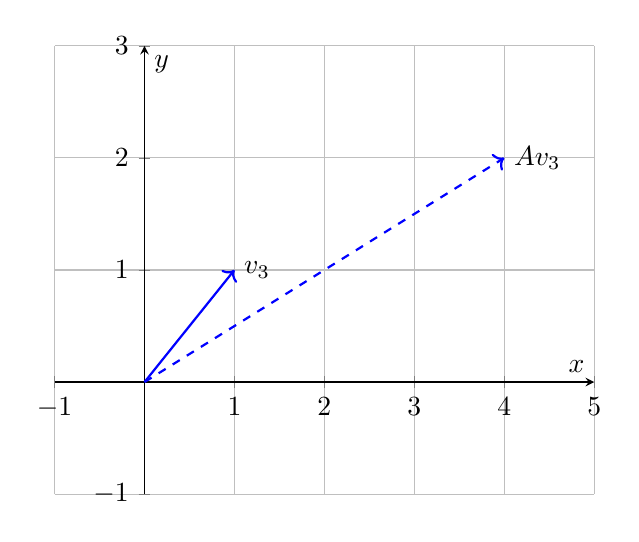
\begin{tikzpicture}
    \begin{axis}[
        axis lines=middle, 
        grid=major, 
        xlabel={$x$}, 
        ylabel={$y$}, 
        ymin=-1, ymax=3,
        xmin=-1, xmax=5
    ]
        % Define original vectors
        \addplot[->, thick, blue] coordinates {(0,0) (1,1)};
        \node[right] at (axis cs:1,1) {$v_3$};

        % Define transformed vectors
        \addplot[->, thick, blue, dashed] coordinates {(0,0) (4,2)};
        \node[right] at (axis cs:4,2) {$A v_3$};
    \end{axis}
\end{tikzpicture}
\end{center}
On remarque que le vecteur $Av_3$ n'est plus situé en même ligne que le vecteur $v_3$, ce qui est logique car si les vecteurs étaient en même lignes après une transformation, cela n'aurait pas de sens.
Par contre, parfois il y'a des cas, quand le vecteur appliqué à la matrice reste en même ligne, par exemple le vecteur $v_2 = \begin{pmatrix} -1 \\ 1 \end{pmatrix} $, avec $Av_2 = \begin{pmatrix} -2 \\ 2 \end{pmatrix} = 2v_2 $

\begin{center}
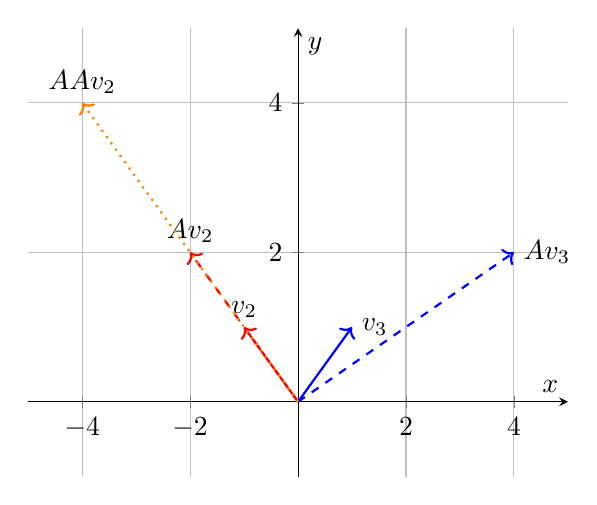
\begin{tikzpicture}
    \begin{axis}[
        axis lines=middle, 
        grid=major, 
        xlabel={$x$}, 
        ylabel={$y$}, 
        ymin=-1, ymax=5,
        xmin=-5, xmax=5
    ]
        % Define original vectors
        \addplot[->, thick, red] coordinates {(0,0) (-1, 1)};
        \node[above] at (axis cs:-1,1) {$v_2$};
        
        \addplot[->, thick, blue] coordinates {(0,0) (1,1)};
        \node[right] at (axis cs:1,1) {$v_3$};

        % Define transformed vectors
        \addplot[->, thick, red, dashed] coordinates {(0,0) (-2,2)};
        \node[above] at (axis cs:-2,2) {$A v_2$};
        
        \addplot[->, thick, blue, dashed] coordinates {(0,0) (4,2)};
        \node[right] at (axis cs:4,2) {$A v_3$};

        \addplot[->, thick, orange, dotted] coordinates {(0,0) (-4,4)};
        \node[above] at (axis cs:-4,4) {$A A v_2$};
    \end{axis}
\end{tikzpicture}
\end{center}
Et c'est pas uniquement le cas du vecteur $\begin{pmatrix} -1 \\ 1 \end{pmatrix} $, en prennant n'importe quel vecteur engendré pas $v = \begin{pmatrix} -1 \\ 1 \end{pmatrix} $, on obtiendra $Av = 2v$.
Tels vecteurs $v$ et les scalaire (ici: 2) sont appelés vecteurs propres et valeurs propres respectivement. Alors, on a la définition formelle:
\begin{definition}
    Soit $f$ un endomorphisme dans  $E$ et un vecteur  $v \in E$ est dit \textbf{vecteur propre} de $f$ si:
     \begin{enumerate}
        \item $v \neq 0$
        \item Il existe un réél $\lambda$ tel que  $f(v) = \lambda v$
    \end{enumerate}
    Le scalaire $\lambda \in \R$ est dit \textbf{valeur propre} correspondante à $v$.
\end{definition}
\begin{intuition}
   Les vecteurs propres sont les vecteurs qui sous l'action de $f$ ne changent pas de diréctions, justement la longueure (même pas toujours). Cela simplifie le calcul de tel vecteurs. Pouvez-vous calculer  $A^3v_3$? Pas très facile, alors le vecteur  $A^3v_2$? 
   \[
    Av_2 = 2v_2 \implies A^2v_2 = 2\cdot 2v_2 = 4v_2 \implies A^3v_2 = 2 \cdot 4v_2 = 8v_2 = \begin{pmatrix} -8 \\ 8 \end{pmatrix} 
   \] 
   C'est cool, n'est-ce pas?
\end{intuition}
Par contre, ce n'est pas la seule utilité des vecteurs propres et on va revenir ici pour en discuter, mais d'abord, comment trouver tels vecteurs?

\section{Recherche des valeurs propres}
On cherche des vecteurs qui sous l'action de l'endomorphisme $f$ sont mis à l'échelle par un facteur de  $\lambda \in \R$, alors on est sensé de résoudre cette équation:
\begin{align*}
    && f(v) &= \lambda v\\
    \iff&& Av &= \lambda v \quad \text{ en notation matricielle}\\
    \iff&& Av &= \lambda (Iv) \quad \text{ où } I \text{ est une matrice identité}\\
    \iff&& Av - \lambda Iv &= 0\\
    \iff&& (A - \lambda I)v &= 0
\end{align*}
Donc, on doit étudier l'application $(A - \lambda I)$ et la connecter à la notion des détérminants. Rappelle: si le détérminant d'une matrice n'est pas nul, cette matrice (i.e endomorphisme) est injective. Dans notre cas, si  $\det(A - \lambda I)$ était nul, le seul vecteur  $v$ qui donnerait  $(A - \lambda I)v = 0$ était le vecteur nul  $v = 0$ car  $(A - \lambda I)$ est linéaire et (comme on a suppoé) injective. 
\par
Par contre, d'après la définition, les vecteurs propres ne sont pas nul, alors le cas injectif ne convient pas, donc pour avoir des vecteurs propres l'application $(A - \lambda I)$ doit ne pas être injectif ce qui équivaut à dire que  $\det(A - \lambda I) = 0$. Alors, on est sensé de calculer le détérminant suivant:
\[
\det(A - \lambda I) = \det \left(\begin{bmatrix} 
    a_{1,1} & a_{1, 2} & \ldots & a_{1, n}\\
    a_{2,1} & a_{2, 2} & \ldots & a_{2, n}\\
    \ldots & \ldots & \ldots & \ldots\\
    a_{n,1} & a_{n,2} & \ldots & a_{n,n}
    \end{bmatrix}  - 
    \begin{bmatrix} 
        \lambda & 0 & \ldots & 0 \\
        0 & \lambda & \ldots & 0 \\
        \ldots & \ldots & \ldots & \ldots\\
        0 & 0 & \ldots & \lambda
    \end{bmatrix}\right) = 
    \begin{vmatrix} 
    a_{1,1} - \lambda & a_{1, 2} & \ldots & a_{1, n}\\
    a_{2,1} & a_{2, 2} - \lambda & \ldots & a_{2, n}\\
    \ldots & \ldots & \ldots & \ldots\\
    a_{n,1} & a_{n,2} & \ldots & a_{n,n} - \lambda
    \end{vmatrix}
\] 
En développant ce détérminant on obtient une équiation du type:
\[
    (-1)^n\lambda^n + a_{n-1}\lambda^{n-1} + \ldots + a_1\lambda + a_0 = 0
\] 
dont les racines sont les valeurs propres de $f$ (rappelle: valeur propre est un facteur $\lambda$).
Ne vous concentrez pas trop sur cette équation pour l'instant, on va y revenir.
\begin{prop}\label{prop:polynome-caracteristique}
   Soit $f$ un endomorphisme dans un espace vectoriel  $E$ de dimension finie  $n$ et $A$ la matrice représentative de  $f$ dans une base de  $E$. Les valeurs propres de  $f$ sont les racine du polynôme:
   \[
   P_f(\lambda) = \det(A - \lambda I)
   \] 
   Ce polynôme est dit \textbf{polynôme caracteristique} de $f$.
\end{prop}
\begin{definition}
    L'ensemble des valeurs propres de $f$ est dit  \textbf{spectre} de $f$ et est noté  $\operatorname{Sp}_K(f)$ ou  $\operatorname{Sp}_K(A)$ si $A$ une matrice de  $f$.
\end{definition}
Pour clarifier:
\begin{eg}
   Soit $f$ un endomorphisme dans  $\R^2$ dont la matrice représentative dans la base canonique est:
   \[
       \begin{bmatrix} 3 & 1\\ 0 & 2 \end{bmatrix} 
   \] 
   Calculons ses valeurs propres:
   \begin{align*}
       && \begin{bmatrix} 3 & 1\\ 0 & 2 \end{bmatrix} v &= \lambda v \\
       \iff && \begin{bmatrix} 3 & 1\\ 0 & 2 \end{bmatrix} v - \lambda I v &= 0\\
       \iff && \left(\begin{bmatrix} 3 & 1\\ 0 & 2 \end{bmatrix}  - \lambda I\right)v  &= 0\\
       \implies && \det \left( \begin{bmatrix} 3 & 1\\ 0 & 2 \end{bmatrix}  - \lambda I \right) &= 0\\
       \implies && \det \left( \begin{bmatrix} 3 & 1\\ 0 & 2 \end{bmatrix}  - \lambda \begin{bmatrix} \lambda & 0\\ 0 & \lambda \end{bmatrix}  \right) &= 0\\
       \implies && \det \left( \begin{bmatrix} 3 - \lambda & 1\\ 0 & 2 - \lambda \end{bmatrix}\right) &= 0\\
                && &= (3-\lambda)(2 - \lambda) = 0
   \end{align*}
   On voit bien, que les solutions sont: $\lambda_1 = 3$ et  $\lambda_2 = 2$
\end{eg}
On peut trouver des valeurs propres, néanmoins, on cherchait les \underline{vecteurs} propres. Et on est là:
\section{Recherche des vecteurs propres}
Supposons pour $q \in \N^{*}$ on a déjà trouvé $q$ valeurs propres d'une matrice $\{ \lambda_1, \ldots, \lambda_q \}$, pour trouver les vecteurs propres, il nous reste à trouver la base de:
\[
    \ker(A - \lambda_iI) \quad \forall i \in \{1, \ldots, q\}
\] 
ce qui équivaut à:
\[
\left( A - \lambda_i I \right)v = 0 \quad \forall i \in \{1, \ldots, q\}
\] 

\begin{eg}
   Encore la matrice  
   \[
       A = \begin{bmatrix} 3 & 1\\ 0 & 2 \end{bmatrix} 
   \] 
   dans la base canonique de $\R^2$. On a déjà trouvé ses vecteurs propres: $\lambda_1 = 3$ et $\lambda_2 = 2$. Alors, cherchons les vecteurs:
   \[
       \begin{bmatrix} 3 - \lambda_1 & 1 \\ 0 & 2 - \lambda_1 \end{bmatrix}\begin{bmatrix} x \\ y \end{bmatrix} = \begin{bmatrix} 3 - 3 & 1 \\ 0 & 2 - 3 \end{bmatrix}\begin{bmatrix} x \\ y \end{bmatrix} = \begin{bmatrix} 0 & 1 \\ 0 & -1 \end{bmatrix}\begin{bmatrix} x \\ y \end{bmatrix} = 0 
       \implies \begin{cases}
           y = 0\\
           -y = 0\\
           x \in \R
       \end{cases}
   \] 
   Donc $\ker(A - 3I) = \begin{pmatrix} x \\ 0 \end{pmatrix} =  \operatorname{Vect}(\begin{pmatrix} 1 \\ 0 \end{pmatrix} )$. Voilà, notre premier vecteur propre: $\begin{pmatrix} 1 \\ 0 \end{pmatrix} $. Pour le deuxième:
   \[
       \begin{bmatrix} 3 - \lambda_2 & 1 \\ 0 & 2 - \lambda_2 \end{bmatrix}\begin{bmatrix} x \\ y \end{bmatrix} = \begin{bmatrix} 3 - 2 & 1 \\ 0 & 2 - 2 \end{bmatrix}\begin{bmatrix} x \\ y \end{bmatrix} = \begin{bmatrix} 1 & 1 \\ 0 & 0 \end{bmatrix}\begin{bmatrix} x \\ y \end{bmatrix} = 0 
       \implies \begin{cases}
           x + y = 0
       \end{cases} \implies \begin{cases}
           x = -y
       \end{cases}
   \] 
   Donc $\ker(A - 2I) = \begin{pmatrix} -y \\ y \end{pmatrix} = y \begin{pmatrix} -1 \\ 1 \end{pmatrix} = \operatorname{Vect}(\begin{pmatrix} -1 \\ 1 \end{pmatrix} )  $ et voilà le deuxieme vecteur propre: $\begin{pmatrix} -1 \\ 1 \end{pmatrix} $ (c'était notre vecteur $v_2$ au début du chapitre).
\end{eg}

Enfin, la propriété utile:
\begin{prop}
    Soit $A \in \mathcal{M}_n(\R)$ avec ses vecteurs propres: $\{\lambda_1, \ldots, \lambda_n\}$, alors:
    \begin{align*}
        &\operatorname{Tr}(A) = \lambda_1 + \ldots + \lambda_n\\
        &\operatorname{det}(A) = \lambda_1 \cdot  \ldots \cdot  \lambda_n\\
    \end{align*}
\end{prop}

\section{Les endomorphismes diagonalisables}
Revenons sur l'utilité des vecteurs propres. Soit $f$ un endomorphisme de  $E$ dont la base est  $\{e_1, \ldots, e_n\}$ et $\operatorname{Mat}_{e_i}(f) = A$ et la matrice de  $f$ dans cette base. Reprennons l'exemple suivant:
 \begin{eg}
     On a: $A = \begin{bmatrix} 3 & 1\\ 0 & 2 \end{bmatrix} $ dans la base canonique $e_1 = \begin{bmatrix} 1 \\ 0 \end{bmatrix} $ et $e_2 = \begin{bmatrix} 0 \\ 1 \end{bmatrix} $. On rappelle qu'on a trouvé deux vecteurs propres:
     \[
     \begin{cases}
         v_1 = \begin{pmatrix} 1 \\ 0 \end{pmatrix} \\
         v_2 = \begin{pmatrix} -1 \\ 1 \end{pmatrix} 
     \end{cases}
     \] 
     On remarque que ces deux vecteurs sont libres et donc forment une base  de $\R^2$. Essayons de changer la base de $A$ dont on a deux façon:
      \begin{enumerate}
          \item On peut calculer les coordonnées de $f(v_1)$ et $f(v_2)$ dans la base $\{v_1, v_2\}$, on a:
              \begin{align*}
                  &f(v_1) = 3v_1 = 3 \cdot v_1 + 0 \cdot v_2\\
                  &f(v_2) = 2v_2 = 0 \cdot v_1 + 2 \cdot v_2
              \end{align*}
              Et alors $\operatorname{Mat}_{v_i}(f) = \|f(v_1), f(v_2)\|_{v_i} = \begin{bmatrix} 3 & 0 \\ 0 & 2 \end{bmatrix} $ 
          \item On peut calculer la matrice $P = P_{e_i \to v_i}$de passage d'une base $\{e_i\}$ vers la base  $\{v_i\}$ et en déduire la matrice de $f$ dans la nouvelle base. On a:
             \[
            \begin{cases}
                v_1 = \begin{pmatrix} 1 \\ 0 \end{pmatrix} = 1 \cdot e_1 + 0 \cdot e_2 = \begin{pmatrix} 1 \\ 0 \end{pmatrix}_{e_i} \\
                v_2 = \begin{pmatrix} -1 \\ 1 \end{pmatrix} = -1 \cdot e_1 + 1 \cdot e_2 = \begin{pmatrix} -1 \\ 1 \end{pmatrix}_{e_i} \\
            \end{cases}
            \] 
              donc $P = \begin{bmatrix} 1 & -1\\ 0 & 1 \end{bmatrix} $ et $P^{-1} = \begin{bmatrix} 1 & 1 \\ 0 & 1  \end{bmatrix}$ (vous pouvez vérifier le calcul). Et donc:
              \[
                  A' = P^{-1}AP = \begin{bmatrix} 1 & 1 \\ 0 & 1 \end{bmatrix} \begin{bmatrix} 3 & 1 \\ 0 & 2 \end{bmatrix} \begin{bmatrix} 1 & -1 \\ 0 & 1 \end{bmatrix} = \begin{bmatrix} 1 & 1 \\ 0 & 1 \end{bmatrix} \underbrace{\begin{bmatrix} 3 & -2 \\ 0 & 2 \end{bmatrix}}_{AP} = \begin{bmatrix} 3 & 0 \\ 0 & 2 \end{bmatrix} 
              \] 
     \end{enumerate}
     Et voilà, la magie, on a trouvé la matrice diagonale.
\end{eg}
Ensuite, généralisons ce qu'on a fait. 
\begin{definition}
    Soit $\lambda \in K$, on note:
    \[
        E_{\lambda} := \{v \in E \mid f(v) = \lambda v \}
    \] 
    $E_{\lambda}$ est un espace vectoriel de $E$ dit  \textbf{espace propre} correspondant à $\lambda$.
\end{definition}
\begin{remark}
   \begin{enumerate}
       \item Si $\lambda$ n'est pas valeur propre de $f$, donc  $E_\lambda = \{0\}$
       \item Si  $\lambda$ est valeur propre, alors:
            \[
                E_\lambda = \{ \text{ vecteurs propres associés à } \lambda \} \cup \{0\} \text{ et } \dim E_\lambda \ge 1
           \] 
   \end{enumerate} 
\end{remark}

\begin{prop}
    Soient $\lambda_1, \ldots, \lambda_p$ des scalaires deux à deux distincts. Alors les espaces propres $E_{\lambda_1}, \ldots, E_{\lambda_p}$ sont en somme directe. Autrement dit, si $\mathcal{B}_1, \ldots, \mathcal{B}_p$ sont des bases de $E_{\lambda_1}, \ldots, E_{\lambda_p}$, la famille $\{\mathcal{B}_1, \ldots, \mathcal{B}_p\}$ est libre (mais pas nécessairement génératrice de $E$).
\end{prop}
\begin{preuve}
Soient $E_{\lambda_1}, \ldots, E_{\lambda_p}$ les espaces propres associés aux valeurs propres $\lambda_1, \ldots, \lambda_p$ d’un endomorphisme $f$ d’un espace vectoriel E. Nous devons montrer que ces sous-espaces sont en somme directe, c’est-à-dire que si un vecteur appartient à leur intersection, alors il est nul.

Prenons un élément v appartenant à leur somme, c’est-à-dire qu’il peut s’écrire sous la forme :
\[
    v = v_1 + v_2 + \cdots + v_p
\] 
avec $v_i \in E_{\lambda_i}$ pour tout $i$.

Puisque chaque $v_i$ est un vecteur propre pour $f$ associé à $\lambda_i$, on a :
\[
    f(v_i) = \lambda_i v_i.
\] 
Appliquons f à la somme :
\[
    f(v) = f(v_1 + v_2 + \cdots + v_p) = f(v_1) + f(v_2) + \cdots + f(v_p).
\] 
En utilisant la linéarité de $f$, cela donne :
\[
    f(v) = \lambda_1 v_1 + \lambda_2 v_2 + \cdots + \lambda_p v_p.
\] 
Or, $v$ est aussi une combinaison de ces mêmes vecteurs :
\[
    v = v_1 + v_2 + \cdots + v_p.
\] 
Donc, en réarrangeant :
\[
    (\lambda_1 v_1 + \lambda_2 v_2 + \cdots + \lambda_p v_p) - (v_1 + v_2 + \cdots + v_p) = 0.
\] 
Ce qui donne :
\[
    (\lambda_1 - 1) v_1 + (\lambda_2 - 1) v_2 + \cdots + (\lambda_p - 1) v_p = 0.
\] 
Factorisons chaque terme :
\[
    (\lambda_1 - \lambda) v_1 + (\lambda_2 - \lambda) v_2 + \cdots + (\lambda_p - \lambda) v_p = 0.
\] 
Or, les $\lambda_i$ sont supposés deux à deux distincts. On en déduit que les coefficients sont différents, et que la somme est nulle uniquement si tous les $v_i$ sont nuls (puisque les espaces propres sont en général en somme directe).

Ainsi, $v = 0$, ce qui prouve que les espaces propres sont en somme directe.
\end{preuve}
Ainsi, les espaces propres sont toujours en sommes directe, mais pas necessairement égale à $E$:
 \[
     E_{\lambda_1} \oplus \ldots \oplus E_{\lambda_p} \underset{\neq}{\subset} E
\] 
ce qu'on a si:
\[
\dim E_{\lambda_1} + \ldots + \dim E_{\lambda_p} < \dim E
\] 

\begin{theorem}
    Soit $f$ un endomorphisme dans  $E$ et  $\lambda_1, \ldots, \lambda_p$ ses valeurs propres, alors les propriétés suivantes sont équivalentes:
    \begin{enumerate}
        \item $f$ est diagonalisable
        \item  $E$ est somme directe de ses espaces propres:  $E = E_{\lambda_1} \oplus \ldots \oplus E_{\lambda_p}$
        \item $\dim E_{\lambda_1} + \ldots + \dim E_{\lambda_p} = \dim E$
    \end{enumerate}
\end{theorem}
\begin{corollary}
   Si $f$ est un endomorphisme de  $E$ avec  $\dim E = n$ et  $f$ admet  $n$ valeurs propres  deux à deux distinctes, alors $f$ est diagonalisable.
\end{corollary}

Mais comme les valeurs propres sont les racines du polynôme caracteristique (voir prop \ref{prop:polynome-caracteristique}) on a:
\begin{prop}
   Soit $f$ un endomorphisme dans $E$ et  $\lambda$ une valeur propre d'ordre  $\alpha$ (i.e $\alpha$ est une racine de  $P_f(\lambda)$ d'ordre  $\alpha$, i.e  $P_f(\lambda) = (X - \lambda)^nQ(X)$ avec  $n \in \N^*$). Alors:
   \[
   \dim E_{\lambda} \le \alpha
   \] 
\end{prop}
\begin{theorem}
   Soit $f$ un endomorphisme dans  $E$ avec $\dim E = n$. Alors  $f$ est diagonalisable si et seulement si: 
   \begin{enumerate}
       \item $P_f(X)$ est \underline{scindé}, i.e:
            \[
                P_f(X) = (-1)^n (X - \lambda_1)^{\alpha_1} \cdot \ldots \cdot (X - \lambda_p)^{\alpha_p}
           \] 
           ($\lambda_i$ sont les racines donc les valeurs propres) et $\alpha_1 + \ldots + \alpha_p = n$. Alors, si la somme des multiplicités des racines est égale à la dimension de l'éspace vectoriel.
       \item Les dimensions des espaces propres sont \underline{maximales}, i.e $\forall i \in \{1, \ldots, p\}$
           \[
                \dim E_{\lambda_i} = \alpha_i 
           \] 
   \end{enumerate}
\end{theorem}
\begin{intuition}
   Ce n'est pas toujours facile de comprendre l'idée par les polynômes caracteristiques, alors une autre façon de voir ça est:
   \begin{enumerate}
       \item On trouve les valeurs propres: $\lambda_1, \ldots, \lambda_p$
       \item Puis on trouve les espaces propres: $E_{\lambda_i} = \ker(f - \lambda_i I)$
       \item On somme les dimension: $\dim E_{\lambda_1} + \ldots + \dim E_{\lambda_p} =: d$.  
           \begin{itemize}
               \item 
                   Si $d = \dim E$ i.e si la somme des dimension est égale à la dimension de l'espace  $E$, les espaces propres engendrent  $E$ et donc  $f$ est diagonalisable (car sa matrice peut s'écrire dans la base de ces vecteurs propres).
              \item Sinon le nombre de vecteurs propres libres ne suffit pas pour engendrer  $E$.
           \end{itemize}
   \end{enumerate}
\end{intuition}

\section{Les applications}
\subsection{Calcul de la puissance}
Alors, on est revenu là, où on a commencé, je vous rappele l'exercice du début du chapitre:
\begin{ex}
   Calculer 
   \[
   \begin{bmatrix} 
       3 & 1\\
       0 & 2
   \end{bmatrix}^{15} = \underbrace{
       \begin{bmatrix} 
       3 & 1\\
       0 & 2
       \end{bmatrix}
       \cdot
       \ldots
       \cdot
       \begin{bmatrix} 
       3 & 1\\
       0 & 2
       \end{bmatrix}
   }_{15 \text{ fois}}
   \] 
On rappelle, que les vecteurs propres de $A$ sont: 
\[
v_1 = \begin{pmatrix} 1 \\ 0 \end{pmatrix} \text{ et } v_2 = \begin{pmatrix} -1 \\ 1 \end{pmatrix} 
\] 
qui sont libres et engendrent $\R^2$ alors forment une base de $\R^2$, alors on peut écrire à dans cette nouvelle base et comme on a déjà trouvé:

\[
    A' = P^{-1}AP = \begin{bmatrix} 1 & 1 \\ 0 & 1 \end{bmatrix} \begin{bmatrix} 3 & 1 \\ 0 & 2 \end{bmatrix} \begin{bmatrix} 1 & -1 \\ 0 & 1 \end{bmatrix} = \begin{bmatrix} 3 & 0 \\ 0 & 2 \end{bmatrix} 
\] 
dans la base $(v_1, v_2)$ avec la matrice de passage:
\[
    P = \begin{bmatrix} 1 & -1\\ 0 & 1 \end{bmatrix} \text{ et } P^{-1} = \begin{bmatrix} 1 & 1 \\ 0 & 1  \end{bmatrix}
\] 
De plus, en multipliant $A'$ avec $A'$, on a:  
\[
    A' \cdot A' = (P^{-1}AP)(P^{-1}AP) = P^{-1}A^2P = A'^2
\] 
d'où
\[
    A'^n = P^{-1}A^{n}P \implies PA'^nP^{-1} = PP^{-1}A^{n}PP^{-1} = A^{n}
\] 
Cela nous donne la possibilité de calculer d'abord la puissance de $A'$:
 \[
     A'^{15} = \begin{bmatrix} 3 & 0 \\ 0 & 2 \end{bmatrix}^{15} = \begin{bmatrix} 3 & 0 \\ 0 & 2 \end{bmatrix}\begin{bmatrix} 3 & 0 \\ 0 & 2 \end{bmatrix}\begin{bmatrix} 3 & 0 \\ 0 & 2 \end{bmatrix}^{13} = \begin{bmatrix} 3^2 & 0 \\ 0 & 2^2 \end{bmatrix}\begin{bmatrix} 3 & 0 \\ 0 & 2 \end{bmatrix}^{13} = \begin{bmatrix} 3^{15} & 0 \\ 0 & 2^{15} \end{bmatrix}
\] 
Voilà, beaucoup plus facile, que calculer $A^15$ directement, alors il nous reste à revenir en base canonique:
 \[
     P \begin{bmatrix} 3^{15} & 0 \\ 0 & 2^{15} \end{bmatrix} P^{-1} = \begin{bmatrix} 1 & -1 \\ 0 & 1 \end{bmatrix} \begin{bmatrix} 3^{15} & 0 \\ 0 & 2^{15} \end{bmatrix}\begin{bmatrix} 1 & 1 \\ 0 & 1 \end{bmatrix} = \begin{bmatrix} 3^{15} & 3^{15} - 2^{15} \\ 0 & 2^{15}\end{bmatrix} 
\] 
\end{ex}
Ce qui est très utile dans les matrices diagonales, c'est que la puissance de telle matrice égale à la même matrice avec les éléments diagonaux pris à la puissance, i.e:
\[
    A' = \begin{bmatrix} 
        \lambda_1 & 0 & \ldots & 0\\ 
        0 & \lambda_2 & \ldots & 0\\
        \vdots & \ddots & \ddots & \vdots\\
        0 & 0 & \ldots & \lambda_n
    \end{bmatrix} \implies A'^{n} = \begin{bmatrix} 
        \lambda_1 & 0 & \ldots & 0\\ 
        0 & \lambda_2 & \ldots & 0\\
        \vdots & \ddots & \ddots & \vdots\\
        0 & 0 & \ldots & \lambda_n
    \end{bmatrix}^{n} = \begin{bmatrix} 
        \lambda_1^n & 0 & \ldots & 0\\ 
        0 & \lambda_2^n & \ldots & 0\\
        \vdots & \ddots & \ddots & \vdots\\
        0 & 0 & \ldots & \lambda_n^n
    \end{bmatrix}
\] 
Généralisons: Si $A \in \mathcal{M}_n(K)$ est diagonalisable (i.e  il existe $P$ et  $A'$ telles que  $A' = P^{-1}AP$), alors:
\[
    A^{n} = P(A'^{n})P^{-1} = P\begin{bmatrix} 
        \lambda_1^n & 0 & \ldots & 0\\ 
        0 & \lambda_2^n & \ldots & 0\\
        \vdots & \ddots & \ddots & \vdots\\
        0 & 0 & \ldots & \lambda_n^n
    \end{bmatrix}P^{-1}
\] 

% \begin{tikzpicture}
%     \begin{axis}[
%         axis lines=middle, 
%         grid=major, 
%         xlabel={$x$}, 
%         ylabel={$y$}, 
%         title={Eigenvector Transformation},
%         ymin=-2, ymax=5,
%         xmin=-3, xmax=5
%     ]
%         % Define original vectors
%         \addplot[->, thick, red] coordinates {(0,0) (1,0)};
%         \node[right] at (axis cs:1,0) {$v_1$};
%
%         \addplot[->, thick, red] coordinates {(0,0) (-1, 1)};
%         \node[above] at (axis cs:-1,1) {$v_2$};
%
%         \addplot[->, thick, blue] coordinates {(0,0) (1,1)};
%         \node[right] at (axis cs:1,1) {$v_3$};
%
%         \addplot[->, thick, blue] coordinates {(0,0) (-1,2)};
%         \node[left] at (axis cs:-1,2) {$v_4$};
%
%         % Define transformed vectors
%         \addplot[->, thick, red, dashed] coordinates {(0,0) (3,0)};
%         \node[right] at (axis cs:3,0) {$A v_1$};
%
%         \addplot[->, thick, red, dashed] coordinates {(0,0) (-2,2)};
%         \node[above] at (axis cs:-2,2) {$A v_2$};
%
%         \addplot[->, thick, blue, dashed] coordinates {(0,0) (4,2)};
%         \node[right] at (axis cs:4,2) {$A v_3$};
%
%         \addplot[->, thick, blue, dashed] coordinates {(0,0) (-1,4)};
%         \node[left] at (axis cs:-1,4) {$A v_4$};
%     \end{axis}
% \end{tikzpicture}


\chapter{Fonctions de plusieurs variables}
\underline{Cadre:} $\R^n, \R^p$ $D \subset \R^n$
\[
F:D \to \R^p
\] 
sur $\R^n$, $\R^p$ distances usuelles, sur $D$ la distance héritée de  $\R^n$.
% \begin{figure}[ht]
%     \centering
%     \incfig{d-distance-exemple}
%     \caption{d-distance-exemple}
%     \label{fig:d-distance-exemple}
% \end{figure}

avec des coordonnées cartésiennes
\[
F(x_1, \ldots, x_n) = (F_1(x_1, \ldots, x_n), F_2(x_1, \ldots, x_n), \ldots, F_p(x_1, \ldots, x_n))
\] 
où $F_i: D \to \R$

\[
F: D \to \R^p \text{ continue}
\] 

on connaît:
\begin{lemma}
   \[
   F: D \to  \R^p \text{ continue ssi:}
   \]  
   chaque $F_i: D \to \R$ est continue
\end{lemma}
\begin{preuve}
    $Y_n = (Y_{1,n}, \ldots, Y_{p, n})$  suite des $\R^p$. $Y_n \to Y$ ssi $Y_{i,n} \to Y_i$ ($1 \le i \le p$)
\end{preuve}

\section{Polynômes annulateurs}
Dans les sections précédentes, on a appris que pour savoir si une matrice est diagonalisable, il faut étudier les espaces propres, ce qui n'est pas toujours très facile et n'est pas la façon la plus vite. Alors, dans cette section on va voir une des autres méthodes d'études de diagonalisabilité, l'une de ces méthodes est l'étude des polynôme annulateurs.

\begin{remark}
   Dans cette section j'écris pas la plupart des preuves mais plutôt l'intuition pourquoi c'est vrai et pourquoi ça marche. 
\end{remark}

\begin{definition}\label{def:polynome-annulateur}
    Soit $f \in \mathbb{K}^n$ un endomorphisme. Un polynôme $Q(X) \in K[X]$ est un \textbf{polynôme annulateur} de $f$ si  $Q(f) = 0$.
\end{definition}
\begin{eg}
   Soit $f$ une projection, alors, on sait que $f^2 = f$, d'où $f^2 - f = 0$, donc  $Q(X) = X^2 - X = X(X - 1)$ est un polynôme annulateur de  $f$.
\end{eg}

Ce qui est important, c'est que les polynômes annulateurs sont très liés aux valeurs propres:
\begin{prop}
   Soit $Q(X)$ est un polynôme annulateur de  $f$, alors les valeurs propres de  $f$ figurent parmis les racines de  $Q$, i.e:
   \[
       \operatorname{Sp}(f) \subset \operatorname{Rac}(Q)
   \] 
\end{prop}
\begin{preuve}
    Soit $Q(X) = a_n X^n + a_{n-1} X^{n-1} + \ldots + a_0$ un polynôme annulateur de $f$ et  $\lambda$ une valeur propre de  $f$. Donc  $\exists v \neq 0 \in E$ tq $f(v) = \lambda v$, de plus:
    \[
        Q(f) = a_n f^n + a_{n-1} f^{n-1} + \ldots + a_0 \operatorname{Id} = 0
    \] 
    Or $f(v) = \lambda v$, donc  $f^2(v) = f(\lambda v) = \lambda^2 v$, d'où  $f^k(v) = \lambda^k v$  $\forall k \in \N$, alors:
    \[
        Q(f(v)) = 0 = (a_n f^n + a_{n-1} f^{n-1} + \ldots + a_0 \operatorname{Id})v = (a_n \lambda^n + a_{n-1} \lambda^{n-1} + \ldots + a_0 \operatorname{Id})v = 0
     \] 
     Or $v \neq 0$, donc $a_n \lambda^n + a_{n-1} \lambda^{n-1} + \ldots + a_0 \operatorname{Id} = 0$ d'où  $\lambda$ est une racine de  $Q$.
\end{preuve}
\begin{note}
    Par contre, l'égalité n'est vrai en général, par exemple $\operatorname{Id}^2 = \operatorname{Id}$, donc  $Q(X) = X^2 - X = X(X - 1)$ annule $\operatorname{Id}$ avec les racines  $0$ et  $1$, mais  $0$ n'est pas une valeur propre de  $\operatorname{Id}$.
\end{note}

\begin{theorem}\label{thm:cayley-hamilton} \textbf{de Cayley-Hamilton}. Soit $f \in K^n$ un endomorphisme et $P_f(X)$ son polynôme caractéristique, alors
     \[
    P_f(f) = 0
    \] 
    Autrement dit, le polynôme caractéristique d'un endomorphisme est son polynôme annulateur.
\end{theorem}
% TODO: preuve <15-04-25, dobbikov> %
\begin{intuition}
   Le polynôme caractéristique nous décrit la structure de $f$, i.e quelles operations il faut faire pour perdre au moins une dimension, si on obtient des facteurs de la forme $(X - \lambda)^n$ donc il faut appliquer  $f(v) - \lambda v) = v_r$, et puis au résultat $v_r$ encore, i.e  $f(v_r) - \lambda v_r$, et on répéte  $n$ fois (ça arrive dans les cas des matrices trigonalisables) 

   Le théorème reste vrai même dans les cas où l'endomorphisme n'est pas trigonalisables car on peut choisir la cloture $K'$ de corp  $K$ dans lequel est notre endomorphisme et il devient trigonalisables (e.g $\mathbb{C}$ pour  $\mathbb{R}$).

   De plus, polynôme caractéristique nous donne  $\ker(P_f(X)) = E$, i.e les vecteurs qui deviennent nuls sous l'action de  $P_f(f)$, le fait intéressant, c'est que tous les vecteurs de  $E$ appartiennent à ce kernel, et donc  $\forall v \in E$, $p_f(f)v = 0$, d'où  $p_f(f) = 0$.
\end{intuition}

\begin{definition}
    Soit $Q$ un polynôme scindé:
     \[
         Q(X) = (X - a_1)^{\alpha_1} \cdots (X - a_r)^{\alpha_r}
    \] 
    Le polynôme 
    \[
    Q_1 = (X - a_1) \cdots (X - a_r)
    \] 
    est appelé \textbf{radical} de $Q$ (i.e polynôme scindé (le même polynôme mais sans puissances à côté des paranthèses). 
    \par De plus, $Q_1 \mid Q$ i.e radical d'un polynôme divise le polynôme lui-même.
\end{definition}
\begin{prop}
    Soit $f$ est un endomorphisme et 
     \[
         P_f(X) = (-1)^n(X - \lambda_1)^{\alpha_1} \cdots (X - \lambda_p)^{\alpha_p}
    \] 
    est son polynôme caractéristique. Alors, si $f$ est diagonalisable, le radical  $Q_1$ annule  $f$ aussi, i.e
     \[
    Q_1(f) = (f - \lambda_1) \cdots (f - \lambda_r) = 0
    \] 
\end{prop}
\begin{intuition}
   Je donne l'intuition de la preuve. Si $f$ est diagonalisable avec un polynôme caractéristique
     \[
         P_f(X) = (-1)^n(X - \lambda_1)^{\alpha_1} \cdots (X - \lambda_p)^{\alpha_p}
    \] 
    avec $r := \alpha_i > 1$ cela \underline{ne signifie pas} qu'il faut appliquer $(f - \lambda_i \operatorname{Id})$  $r$ fois pour réduire la dimesion comme dans le cas des matrices trigonalisables, mais cela signifie que  $E_{\lambda_i}$ l'espace propre de valeur propre  $\lambda_i$ est de dimension  $\alpha_i = r$ et donc $\forall v \in E_{\lambda_i}, f(v) = \lambda_i v$. 

    Comme $E = E_{\lambda_1} \oplus \ldots \oplus E_{\lambda_p}$, si $v \in E$, donc $\exists i \in \{1, \ldots, p\}$ tq $v \in E_{\lambda_i}$ et donc $f(v) - \lambda_i v = 0$ i.e  $(f - \lambda_i \operatorname{Id})(v) = 0$. D'où le radical de $P_f$ annule  $f$.
\end{intuition}
\section{Le Lemme des noyaux}
\begin{lemma}\label{lemma:lemme-des-noyaux} \textbf{des noyaux}
   Soit $f \in K^n$ un endomorphisme et 
   \[
   Q(X) = Q_1(X) \cdots Q_p(X)
   \] 
   un polynôme factorisé en produit de polynômes deux à deux premiers entre eux. Si $Q(f) = 0$ alors:
    \[
        E = \operatorname{Ker} Q_1(f) \oplus \ldots \oplus \operatorname{Ker} Q_p(f)
   \] 
\end{lemma}
\begin{intuition}
    Comme $Q(f) = 0$, donc  $\forall v \in E, Q(f)(v) = 0$ donc
    $\operatorname{Ker}(Q(f)) = E$. $\exists v_1, \ldots, v_p$ tq $v = v_1 +
    \ldots + v_p$. Or tous les polynômes sont deux à deux premiers, alors c'est
    seulement l'un qui annule $v_i$ donc  $v_i \in \operatorname{Ker}Q_i(f)$ et
    cela reste vrai pour tous les $v_1, \ldots, v_p$. Et comme les polynômes
    sont premiers, donc si $k \neq j$ et $Q_k(v_i) = 0$, donc  $Q_j(v_i) \neq
    0$ car $Q_j$ et  $Q_k$ sont différents. Alors,  $\forall i, j \,
    \operatorname{Ker}Q_i \cap \operatorname{Ker}Q_j = \{0\}$.
\end{intuition}
\begin{remark}
   Revenons sur l'exemple de $f$ qui est une projection, donc  $f^2 - f = 0$ et  $Q(X) = X^2 - X = X(X-1)$ annule $f$. Or  $X$ et  $X-1$ sont premiers entre eux, alors 
    \[
        E = \operatorname{Ker}f \oplus \operatorname{Ker}(f - \operatorname{Id})
   \] 
    Pour être plus générale, soit $f$ un endomorphisme et $Q(X) = (X - \lambda_1) \cdots (X - \lambda_p)$ tq $Q(f) = 0$, on a:
     \[
         E = \underbrace{\operatorname{Ker}(f - \lambda_1 \operatorname{Id})}_{E_{\lambda_1}} \oplus \ldots \oplus \underbrace{\operatorname{Ker}(f - \lambda_p \operatorname{Id})}_{E_{\lambda_p}}
    \] 
    Bien sur, $\lambda_i \neq \lambda_j$. Et alors $f$ est diagonalisable car somme directe de ces espaces propres.
\end{remark}
\begin{corollary}
    Un endomorphisme $f$ est diagonalisable si et seulement s'il existe un polynôme annulateur  $Q$ de  $f$ scindé et n'ayant que des racines simples \footnote{scindé: $(X - \lambda_i)^{\alpha_i}$ - $X$ est à la puissance  $1$! racines simples: si  $\alpha_i = 1$ aussi i.e les facteurs  $(X - \lambda)$ sont à la puissance 1!} 
\end{corollary}

\section{Recherche des polynômes annulateurs. Polynôme minimal}
\begin{definition}
    On appelle un  \textbf{polynôme minimal} de $f$ noté  $m_f(X)$ - le polynôme normalisé \footnote{i.e de coefficient $1$ du terme du plus haut degré, i.e:  $1*X^n + a_{n-1}X^{n-1} + \ldots + a_0$} qui annule $f$ de degré le plus petit.
\end{definition}
\begin{prop}
   Les polynômes annulateurs de $f$ sont le polynômes de la forme:
   \[
       Q(X) = A(X)m_f(X) \quad \text{ avec } \quad A(X) \in K[X]
   \] 
   i.e $m_f(X)$ divise  $Q(X)$. 
\end{prop}
\begin{prop}
   Les racines du polyôme minimal $m_f(X)$ sont exactement les racines du polynôme caractéristique  $P_f(X)$, c'est-à-dire les valeurs propres.
\end{prop}
\begin{preuve}
   On sait que $P_f(X) = A(X)m_f(X)$ donc si  $\lambda$ est une racine de  $m_f(X)$,  alors elle est racine de  $P_f(X)$ aussi. Réciproquement, si $\lambda$ est une racine de  $P_f(X)$ alors elle une valeur propre, or  $m_f(X)$ annule  $f$, donc  $\lambda$ est aussi une racine de  $m_f(X)$.
\end{preuve}
\begin{theorem}
    Un endomorphisme $f$ est diagonalisable si et seulement si son polynôme minimal est scindé et il a toutes ses racines simples.
\end{theorem}
\begin{eg}
   \begin{enumerate}
       \item $A = \begin{pmatrix} 
            -1 & 1 & 1\\
            1  & -1 & 1\\
            1  & 1  & -1
           \end{pmatrix} $. $P_A(X) = -(X - 1)(X + 2)^2$, donc on a deux possibilité:
           \begin{itemize}
               \item $m_A(X) = (X - 1)(X + 2)$ - donc  $A$ diagonalisable
               \item  $m_A(X) = (X - 1)(X + 2)^2$ - donc $A$ pas diagonalisable
           \end{itemize}
           Calculons:
           \[
            (A - I)(A + 2I) = \begin{pmatrix} 
                -2 & 1 & 1\\
                1 & -2 & 1\\
                1 & 1  & -2
            \end{pmatrix}\begin{pmatrix} 
                1 & 1 & 1\\
                1 & 1 & 1\\
                1 & 1 & 1
            \end{pmatrix} = \begin{pmatrix} 
                0 & 0 & 0\\
                0 & 0 & 0\\
                0 & 0 & 0
            \end{pmatrix}   
           \] 
           Donc, $m_f(X) = (X - 1)(X + 2)$ et donc  $A$ est diagonalisable.
        \item  $A = \begin{pmatrix} 
                3 & -1 & 1\\
                2 & 0  & 1\\
                1 & -1 & 2
            \end{pmatrix} $. On a: $P_A(X) = -(X - 1)(X - 2)^2$, donc:
            \[
            m_A(X) = \begin{cases}
                (X-1)(X-2) \quad \text{ i.e $A$ diagonalisable}\\
                (X-1)(X-2)^2 \quad \text{ i.e $A$ pas diagonalisable}
            \end{cases}
            \] 
            Calculons:
            \[
                (A - I)(A - 2I) = \begin{pmatrix} 
                    2 & -1 & 1\\
                    2 & -1 & 1\\
                    1 & -1 & 1\\
                \end{pmatrix} 
                \begin{pmatrix} 
                    1 & -1 & 1\\
                    2 & -2 & 1\\
                    1 & -1 & 0
                \end{pmatrix} 
                =
            \begin{pmatrix}
            1 & -2 & 1 \\
            1 & -2 & 1 \\
            0 & -2 & 2
            \end{pmatrix} \neq \begin{pmatrix} 0 & 0 & 0\\  0 & 0 & 0\\ 0 & 0 & 0 \end{pmatrix} 
            \] 
            D'où $m_A(X) \neq (X-1)(X-2)$ et donc $A$ n'est pas diagonalisable.
   \end{enumerate} 
\end{eg}


\chapter{Dérivation des fonctions de plusieurs variables}
\section{Introduction}
$n = 1$: comment définir  $f'(x_0)$?
\begin{enumerate}
    \item $f'(x_0) = \lim_{x \to x_0} \frac{f(x) - f(x_0)}{x - x_0}$
    \item DL: $f(x) = f(x_0) + a_1(x - x_0) + (x - x_0)\epsilon(x)$ où $a_1 = f'(x_0)$
\end{enumerate}

\[
f: D \to R \quad D \text{ ouvert } \quad X_0 \in D \quad D \subset \R^n
\] 

\begin{definition}
    $f$ est dérivable en  $X_0$ dans la direction $\vec{u}$ $(\neq \vec{0})$ si la fonction
    \begin{align*}
        g: \R &\longrightarrow \R \\
        t &\longmapsto g(t) = f(X_0 + t\vec{u})
    .\end{align*}
    est dérivable en $t = 0$
\end{definition}
Autrement dire, la dérivée directionnelle (dans la direction de vecteur $\vec{u}$) est donnée par:
\begin{equation}\label{eq:derivee-directionnelle}
    D_{u}f(X_0) = \lim_{t \to 0} \frac{f(X_0 + t\vec{u}) - f(X_0)}{t}
\end{equation}
Dans le cas $\R$ on a eu la définition de la dérivée:
\[
f'(x_0) = \lim_{t \to 0} \frac{f(x_0 + t) - f(x_0)}{t} 
\] 
La diréction était toujours la même (l'axe $x$), on peut voir ça comme prendre un vecteur $u = (1)$ et utiliser comme la direction seulement l'axe $x$ et on obtient  l'eq. (~\ref{eq:derivee-directionnelle})
\begin{figure}[H]
    \centering
    \incfig{continuite-multidimensionelle}
    \caption{Dérivée directionnelle}
    \label{fig:continuite-multidimensionelle}
\end{figure}
$\vec{e_1}, \ldots, \vec{e_n}$ base canonique de $\R^n$, $f$ admet des dérivées partielles en  $X_0$ si $f$ dérivable en  $X_0$ dans les directions $\vec{e_1}, \ldots, \vec{e_n}$.
\[
    \frac{d}{dt} f(X_0 + t \vec{e_i}) \mid_{t = 0}
\] 
noté
\[
\frac{\partial f}{\partial x_i}(X_0)
\] 
Par contre, une fonction peut être dérivable dans \underline{toutes les diréctions} en un point mais \underline{ne pas être} continue en ce point, voici 

\begin{eg}
   \[
   f(x_1, x_2) = \begin{cases}
       1  \text{ si } x_2 = x_1^2 \text{ et } (x_1, x_2) \neq (0, 0)\\
       0 \text{ sinon}
   \end{cases}
   \]  
\begin{figure}[H]
    \centering
    \incfig{exemple-dervie-partielle}
    \caption{Exemple dérivable mais pas continue}
    \label{fig:exemple-dervie-partielle}
\end{figure}
\[
    f((0, 0) + t \vec{u}) = f(t \vec{u}) = 0
\] 
si $t\neq 0$ et $t$ petit, on a $f$ dérivable dans toutes les directions.
\par
Mais, $f$ n'est pas continue en  $(0, 0)$:
 \[
X_n = (\frac{1}{n}, \frac{1}{n^2}) \quad X_n \to (0, 0)
\] 
\[
\forall n, f(X_n) = 1 \quad f(X_n) \not\xrightarrow[n \to \infty]{} f(0, 0)
\] 
\end{eg}

\begin{definition}\label{def:fonction-differentiable}
    Soient $D \subset \R^n$ ouvert et $X_0 \in D$, la fonction
    $f: D \to \R$
    est \textbf{différentiable} en $X_0$ s'il existe un vecteur $\vec{u} \in \R^n$ tel que 
    \[
        f(X_0 + \vec{X}) = f(X_0) + \vec{u} \cdot \vec{X} + \|\vec{X}\|\epsilon(\vec{X})
    \] 
    où $\lim_{\vec{X} \to \vec{0}} \epsilon(\vec{X}) = 0$
\end{definition}
\begin{intuition}
   Je propose de réflechir sur ce que cette définition signifie. 
   Rappelons ce que signifie intuitivement la dérivée au cas $\R^n = \R$ ($n = 1$). 
   Intuitivement, si on zoom la fonction qu'on dérive elle se comporte et a l'air d'être une ligne. 
   Dans le cas $R^n = \R^2$, si on zoom la fonction elle a l'air d'être un plan. 
   En effet, c'est ça l'idée de la dérivée, que si on fait un petit petit pas d'un fourmit, le deplacement et aussi petit et uniforme. 
   En augmentant $n$, la dérivée donne des scalaire pour contruire un sous-éspace de dimension $n-1$ de l'espace $\R^n$. 
\end{intuition}

\section{DL à l'ordre 1}
Cette représentation de la dérivée comme un sous-éspace lorsqu'on zoom est représenté par le DL à l'ordre $1$.
De la définition ~\ref{def:fonction-differentiable}, ce vecteur $\vec{u}$ se note $\vec{\nabla}f(X_0)$ (gradient de $f$ en  $X_0$)

\begin{prop}
   $f$ différentiable en  $X_0$ $\implies$ $f$ dérivable dans toutes les directions en  $X_0$, et alors: 
   \[
       \vec{\nabla}f(X_0) = \begin{pmatrix} \frac{\partial f}{\partial x_1}f(X_0)\\ \ldots \\  \frac{\partial f}{\partial x_n}f(X_0)\end{pmatrix} 
   \] 
   dans la base $\vec{e_1}, \ldots, \vec{e_n}$
\end{prop}

\begin{preuve}
$f$ est continue en  $X_0$ $|\vec{u} \cdot X| \le |\vec{u}| |X|$
\begin{enumerate}
    \item continuité
        \begin{align*}
            |f(X_0 + X) - f(X_0)| &\le |\vec{u} \cdot X| + \|X\| |\epsilon(X)|\\
                                  &\le \|X\|\left( \|\vec{u}\| + |\epsilon(x)|  \right) \le c\|X\|
        \end{align*}
        donc: $f(X_0 + X) \xrightarrow[X \to \vec{0}]{} f(X_0)$
    \item .
        \begin{align*}
            g(t) = f(X_0 + t \vec{v}) &= f(X_0) + \vec{\nabla}f(X_0) \cdot t \vec{v} + \|t \vec{v}\| \cdot \epsilon(t \vec{v})\\
                                      &= f(X_0) + t\vec{\nabla}f(X_0) \cdot \vec{v} + |t|\|\vec{v}\|\epsilon_1(t)\\
                                      &= f(X_0) + t\vec{\nabla }f(X_0)\cdot \vec{v}
        \end{align*}
        donc:
        \[
            \frac{d}{dt} f(X_0 + t\vec{v})\mid_{t = 0} = \vec{\nabla}f(X_0)\cdot \vec{v}
        \] 
        (prendre $\vec{v} = \vec{e_1}, \ldots, \vec{e_n}$ pour les coordonnées de $\vec{\nabla}f(X_0)$)
\end{enumerate}
\end{preuve}
\begin{definition}
    \[
        D \subset \R^n \quad D \text{ ouvert } \quad f: D \to \R \text{ est } \mathcal{C}^1 \text{ sur } D
    \] 
    Soit $D \subset \R^n$ ouvert, alors la fonction $f: D \to \R$ est de classe $\mathcal{C}^1$ sur  $D$ si 
    $f$ est différentiable en tout  $X \in D$ et la fonction
    \begin{align*}
        : D &\longrightarrow \R^n \\
        X &\longmapsto \vec{\nabla}f(X)
    \end{align*}
    est continue.
\end{definition}
\begin{theorem}
    $f$ de classe  $\mathcal{C}^1$ sur  $D$ ssi  $f$ admet des dérivées partielles continues en tout point de  $D$. 
\end{theorem}

\begin{eg}
   \[
       f(X) = f(X_0) + \vec{\nabla}f(X_0) \cdot (X - X_0) + \|X - X_0\| \epsilon(X - X_0)
   \]  
   linéaire
   \par
   Dans $\R^3$: $f(x, y, z)$
    \[
        S = \{(x, y, z): f(x, y, z) = 0 \}
   \] 
   $S$: surface dans  $\R^3$, $X_0 \in S$ plan tangent à $S$ en  $X_0$, plan d'équation:
   \[
       f(X_0) + \vec{\nabla}f(X_0)\cdot X = 0
   \] 
\begin{figure}[H]
    \centering
    \incfig{surface-s-differentiable}
    \caption{Exemple d'une surface differentiable}
    \label{fig:surface-s-differentiable}
\end{figure}
\end{eg}

\section{Extrema et points critiques}
\begin{definition}
    Extremum (local) de $f$ est un minimum ou un maximum (local) de  $f$
    \begin{itemize}
        \item $X_0$ est un maximum local de $f$ si: $\exists \delta > 0$ tel que
            \[
            \forall X \in D, f(X) \le f(X_0) \text{ avec } d(X, X_0) \le \delta
            \] 
        \item $X_0$ est un minimum local de $f$ si: $\exists \delta > 0$ tel que
            \[
            \forall X \in D, f(X) \ge f(X_0) \text{ avec } d(X, X_0) \le \delta
            \] 
    \end{itemize}
\end{definition}

\begin{definition}
    Soit $f: D \to \R$ et $X_0 \in D$, alors si
     \[
         \vec{\nabla}f(X_0) = \vec{0}
    \] 
    donc $X_0$ est un \textbf{point critique}.
\end{definition}
\begin{intuition}
   Le lien entre les extremums et le point critique: 
   \begin{enumerate}
       \item pour que l'extremum existe, il faut qu'il existe au moins un point critique - c'est un critère nécessaire \underline{mais pas suffisant}.
       \item tout extremum local est un point critique
   \end{enumerate}
   Les points critiques falicites la recherche des extremums locaux.
\end{intuition}

\begin{theorem}
    Soit $f: D \longrightarrow \R$ différentiable, $D$ ouvert et  $X_0 \in D$ (sinon, si $D$ pas ouvert, il faut  $X_0 \in \operatorname{Int}(D)$) alors:
    \[
        X_0 \text{ extremum local } \implies X_0 \text{ point critique} 
    \] 
\end{theorem}

\begin{eg} Pas tout point critique est un extremum local
\begin{figure}[H]
    \centering
    \incfig{point-critique-nestpas-extremum-local}
    \caption{Point critique qui n'est pas un extremum local}
    \label{fig:point-critique-nestpas-extremum-local}
\end{figure}
\end{eg}

\section{Dérivées partielles d'ordre $\ge 2$}
\begin{definition}
    Soit $D$, alors  $f: D \to \R$ est $\mathcal{C}^k$ si  $f: D \to \R$ est $\mathcal{C}^1$ et  $\partial_{x_i}f: D \to \R$ sont $C^{k-1}$
\end{definition}

\begin{definition}
    Soient $\alpha = (\alpha_1, \ldots, \alpha_n)$ \quad $\alpha_i \in \N$. On pose
    \[
        \partial_{x}^{\alpha}f = \frac{\partial^{\alpha_1}}{\partial x_1^{\alpha_1}} \cdot \ldots \cdot \frac{\partial^{\alpha_n}}{\partial x_n^{\alpha_n}}
    \] 
    est la notation pour la dérivée d'ordre supérieure.
\end{definition}
\[
    \frac{\partial}{\partial x_1}\frac{\partial}{\partial x_2}\frac{\partial}{\partial x_1} f \overset{?}{=}  \frac{\partial^2}{\partial x_1^2}\frac{\partial}{\partial x_2}f
\] 

\begin{theorem}\label{thm:lemme-de-schwarz}
    Lemme de Schwarz
    \par
    Si $f \in \mathcal{C}^2(D)$ alors 
    \[
        \displaystyle \frac{\partial^2 f}{\partial x_i\partial x_j}(X) = \frac{\partial^2 f}{\partial x_j\partial x_i}(X) \qquad \forall X \in D, \forall i, j
    \] 
\end{theorem}
\begin{eg} où une fonction admet des dérivées partielles d'ordre supérieure mais $\displaystyle \frac{\partial^2 f}{\partial x_i\partial x_j}(X) \neq  \frac{\partial^2 f}{\partial x_j\partial x_i}(X)$
   \[
   f(x_1, x_2) = \begin{cases}
       x_1x_2 \frac{x_1^2 - x_2^2}{x_1^2 + x_2^2} \text{ si } (x_1, x_2) \neq (0, 0)\\
       0 \text{ si } (x_1, x_2) = 0
   \end{cases}
   \]  
   \[
   r^2 \sin(\theta)\cos(\theta)\cos(2\theta) = \frac{1}{4}r^2\sin(4\theta)
   \] 
   On calcule $\displaystyle \frac{\partial^2f}{\partial_{x_1}\partial_{x_2}}(0, 0)$?
       C'est $\displaystyle \frac{\partial}{\partial x_1}g(x_1)$ en $x_1 = 0$ pour $\displaystyle g(x_1) = \frac{\partial f}{\partial x_2}(x_1, x_2)|_{x_2 = 0}$. Calcul de $g(x_1)$:
    \begin{enumerate}
        \item si $x_1 \neq 0$ $\frac{\partial f}{\partial x_2}(x_1, x_2) = x_1 \frac{x_1 ^ 2 - x_2^2}{x_1^2 + x_2^2}$, donc si $x_1 \neq 0$ $\frac{\partial f}{\partial x_2}(x_1, 0) = x_1$ 
        \item si $x_1 = 0$ $f(0, x_2) = 0$
    \end{enumerate}
    Conclusion:
    \[
    \frac{\partial f}{\partial x_2}(x_1, 0) = x_1 \quad \forall x_1
    \] 
    donc: 
    \[
    \frac{\partial}{\partial x_1}\frac{\partial}{\partial x_2}f(0, 0) = 1
    \] 
    $\displaystyle \frac{\partial}{\partial x_2}\frac{\partial}{\partial x_1}f(0, 0) = ?$. On voit que, $f(x_2, x_1) = -f(x_1, x_2)$ donc 
    \[
    \frac{\partial}{\partial x_2}\frac{\partial}{\partial x_1}f(0, 0) = - \frac{\partial}{\partial x_1}\frac{\partial}{\partial x_2}f(0, 0) = -1
    \] 
\end{eg}

\section{Formule de Taylor à l'ordre 2}
\begin{definition}
    Soit $f \in \mathcal{C}^2(D)$. Matrice hessienne: matrice  $n \times n$
    \[
    H_f(X_0) = \begin{bmatrix} \frac{\partial^2}{\partial x_i \partial x_j}(X_0) \end{bmatrix} 1\le i,j \le n
    \] 
    Le lemme \ref{thm:lemme-de-schwarz} nous donne que $H_f(X_0)$ est symmetrique si $f \in \mathcal{C}^2(D)$
\end{definition}
Rappel: 
\[
    \vec{\nabla}f(X_0) = \begin{pmatrix} \frac{\partial f}{\partial x_1}(X_0) \\ \vdots \\ \frac{\partial f}{\partial x_n}(X_0) \end{pmatrix} 
\] 

\begin{theorem} De Taylor à l'ordre 2 \par
    Soit $f \in \mathcal{C}^2(D)$,  $X_0 \in D$. Alors  
    \begin{align*}
        f(X_0 + \vec{X}) = f(X_0) + \vec{\nabla }f(X_0) \cdot \vec{X} + \frac{1}{2}\vec{X} \cdot H_f(X_0)\vec{X}
    \end{align*}
    exemple en $\R^1$
    \[
    f(x_0 + x) = f(x_0) + f'(x_0)x + \frac{1}{2}f''(x_0)x^2 + \ldots
    \] 
\end{theorem}
\begin{intuition}
   Alors, la matrice hessienne sert à calculer la dérivée d'ordre 2. 
\end{intuition}

\section{Un rappel d'algèbre linéaire et le lien avec l'analyse}
\[
    \vec{X} \cdot A\vec{X} = \sum_{1\le i,j \le n}^{} x_ia_{i,j}x_j
\] 
Si $\vec{X} = \begin{pmatrix} x_1 \\ \vdots \\ x_n \end{pmatrix}$ $A = \begin{bmatrix} a_{i,j} \end{bmatrix}$ on a: $X \mapsto X \cdot AX$ à étudier. Si $A = A^T, A \in \mathcal{M}_n(\R)$
\begin{center}
   "$A$ admet une base orthonormée de vecteurs propres" 
\end{center}
Il existe une base $\vec{u_1}, \ldots, \vec{u_n}$ de $\R^n$ avec $\vec{u_i} \cdot \vec{u_j} = \delta_{i, j}$ ($1$ si  $i = j$ et  $0$ sinon) et des réels $\lambda_1, \ldots, \lambda_n$($\lambda_i = \lambda_j$ possible) tels que
\[
    A\vec{u_i} = \lambda_i\vec{u_i}
\] 
\[
    \vec{X} = \sum_{j=1}^{n} y_j\vec{u_j}
\] 
\[
    \vec{X} \cdot \vec{u_i} = \sum_{j=1}^{n} y_j\vec{u_j}\vec{u_i} = y_i
\] 
\begin{align*}
    \|\vec{X}\|^2 = \vec{X} \cdot \vec{X} &= \left( \sum_{j=1}^{n} y_j\vec{u_j} \right) \cdot \left( \sum_{i=1}^{n} y_i\vec{u_i} \right) \\
                                          &= \sum_{j=1}^{n} \sum_{i=1}^{n} y_jy_i\vec{u_j}\cdot \vec{u_i}\\ 
                                          &= \sum_{j=1}^{n} y_j^2
\end{align*}

\begin{align*}
    A\vec{X} = A \sum_{j=1}^{n} y_j\vec{u_j} = \sum_{j=1}^{n} y_jA\vec{u_j} = \sum_{j=1}^{n} \lambda_jy_j\vec{u_j}
\end{align*}
\[
    \vec{X} \cdot A\vec{X} = \sum_{i=1}^{n} \lambda_iy_i^2
\] 
\begin{enumerate}
    \item si $\lambda_i > 0$ ($1 \le i \le n$)
        \[
        C = \min \lambda_i > 0
        \] 
        \[
        X \cdot AX \ge C \sum_{i=1}^{n} y_i^2 = C \|X\|^2
        \] 
    \item si $\lambda_i < 0$ ($1 \le i \le n$)
        \[
        -C = \max \lambda_i < 0
        \] 
        \[
        X \cdot AX \le -C\|X\|^2
        \] 
\end{enumerate}
\begin{eg}
   $n = 2$ 
   \[
   f(y_1, y_2) = -y_1^2 + 3y_2^2
   \] 
   \[
   \lambda_1 = -1 \qquad \lambda_2 = 3
   \] 
   \[
   f(y_1, 0) < f(0, 0) < f(0, y_2)
   \] 
\end{eg}

\section{Nature des points critiques}
\begin{theorem}\label{thm:nature-des-points-critiques}
    (Nature des points critiques) \par
    Soient $f \in \mathcal{C}^2(D)$,  $X_0 \in D$, $D$ ouvert et  $\vec{\nabla }f(X_0) = \vec{0}$
    \begin{enumerate}
        \item si toutes les valeurs propres de $H_f(X_0)$ sont $> 0$ (resp $< 0$) $X_0$ est minimum (resp. maximum) local.
        \item si toutes les valeurs propres de $H_f(X_0)$ sont \underline{non nulles} mais pas de même signe, $X_0$ n'est pas un extremum local: $X_0$ est un point selle (un col).
        \item si 0 valeurs propres de $H_f(X_0)$, pas de conclusion, ($X_0$ point critique dégénéré) i.e on ne peut rien conclure
    \end{enumerate}
\end{theorem}

\begin{preuve} du théorème ~\ref{thm:nature-des-points-critiques}
   \[
       f(X_0 + X) - f(X_0) = \frac{1}{2}X\cdot H_f(X_0)X + \|X\|^2\epsilon(X)
   \]  
   .
   \begin{enumerate}
       \item si $\lambda_i > 0$  $\frac{1}{2}X \cdot H_f(X_0)X \ge C\|X\|^2$ $C > 0$
            \[
           f(X_0 + X) - f(X_0) \ge \|X\|^2(C + \epsilon(X)) \ge \frac{C}{2}\|X\|^2 \text{ si } \|X\| \text{ assez petit }
           \] 
           \[
           \implies X_0 \text{ minimum local}
           \] 
        \item si $\lambda_1 < 0$ et  $\lambda_2 > 0$
             \[
                 H_f(X_0)\vec{u_i} = \lambda_i\vec{u_i}
            \] 
            \[
                f(X_0 + t\vec{u_i}) = f(X_0) + \frac{1}{2} \lambda_it^2 + t^2\epsilon(t)
            \] 
            \[
                \epsilon(t\vec{u_i}) = \epsilon(t)
            \] 
            \[
                f(X_0 + t\vec{u_i}) - f(X_0) = t^2 (\frac{1}{2}\lambda_i + \epsilon(t))
            \] 
            si $i = 1$  $< 0$  $|t|$ petit,  $i = 2$  $> 0$  $|t|$ petit, alors  $X_0$ n'est pas un extremum local
   \end{enumerate}
\end{preuve}

\begin{eg}
   \[
   f(x, y) = \frac{1}{2}(x^2 - y^2)
   \]  
   \[
       H_f(0, 0) = \begin{pmatrix} 1 & 0\\ 0 & -1 \end{pmatrix} 
   \] 
   \[
       I_f = \{(x, y, z): z = \frac{1}{2}(x^2 - y^2)\}
   \] 
\begin{figure}[H]
    \centering
    \incfig{exemple-point-selle}
    \caption{Exemple de point selle.}
    \label{fig:exemple-point-selle}
\end{figure}
Les lignes rouges représentent les dérivées partielles et on voit bien que les uns sont croissants et les autres décroissants, donc ce point n'est ni le minimum ni le maximum
\end{eg}

\begin{eg}
$n = 2$
 \[
A = \begin{pmatrix} 
    a_{1,1} & a_{1, 2}\\
    a_{2, 1} & a_{2, 2}
\end{pmatrix} 
\] 
$(a_{1,2} = a_{2, 1})$
\par
Valeurs propres: racines du pol. Caractéristique:  
\[
    P(\lambda) = \det(A - \lambda I) = \begin{vmatrix} a_{1,1} - \lambda & a_{1, 2} \\ a_{2, 1} & a_{2,2} - \lambda \end{vmatrix} = (\lambda - a_{1,1})(\lambda - a_{2,2}) -  a_{1,2}a_{2,1}
\] 
\[
    \lambda^2 - (a_{1,1} + a_{2,2})\lambda + a_{1,1}a_{2,2} - a_{2,1}a_{1,2}
\] 
\[
    a_{1,1} + a_{2,2} = Tr(A)
\] 
\[
    a_{1,1}a_{2,2} - a_{2,1}a_{1,2} = \det(A)
\] 
\[
    x^2 - Sx + P = x^2 - (\lambda_1 + \lambda_2)x + \lambda_1\lambda_2
\] 
\begin{align*}
    &\det(A) = \text{ produit des valeurs propres}\\
    &Tr(A) = \text{ somme des valeurs propres}
\end{align*}
\[
A = H_f(X_0)
\] 
\begin{enumerate}
    \item si $\det(A) < 0$,  $X_0$ point col
    \item si $\det(A) > 0$
         \begin{enumerate}
            \item $Tr(A) > 0$, $X_0$ minimum
            \item  $Tr(A) < 0$, $X_0$ maximum
        \end{enumerate}
    \item $\det(A) = 0$,  $X_0$ point critique dégénéré
\end{enumerate}
\end{eg}

% \chapter{Espaces vectoriels normés}
Soient:
\begin{itemize}
    \item espace vectoriel $E$,  $F$, etc
    \item vecteurs:  $x, y, e$, etc.
    \item vecteur nul: noté  $0_E$ ou simplement  $0$
    \item scalaires:  $\lambda, \mu \in \mathbb{K}$
    \item  $\mathbb{K} = \R \text{ ou } \mathbb{C}$
    \item $A \in \mathcal{L}(E, F)$ action sur $x$, notée  $Ax$ (plutôt que $A(x)$)
    \item dimension: $E$ de dimension finie si  $E$ admet une base avec un nombre fini d'éléments, sinon  $E$ est dit de dimension infinie  $\iff$ $\forall N \in \N$, il existe une famille libre de $N$ vecteurs. La dimension dépend de  $\mathbb{K}$!
         \begin{itemize}
             \item sur $\mathbb{C}$  $\dim \mathbb{C} = 1$ base formée du vecteur  $1 \in \mathbb{C}$
             \item sur  $\R$ $\dim \mathbb{C} = 2$ base formée de $1, i$
        \end{itemize}
        \begin{align*}
            &z = z \cdot 1 \quad z \in \mathbb{C}\\
            &z = x \cdot 1 + y \cdot i \quad x, y \in \R
        \end{align*}
        \[
            \mathbb{C} \sim \R^2 \text{ comme } \R \text{ espace vectoriel}
        \] 
\end{itemize}

\begin{definition}
    Soit $E$ un  $\mathbb{K}$-espace vectoriel et $\lambda \in \R$, la \textbf{norme} sur  $E$ est une application $N: E \to \R_{+}$ avec:
    \begin{enumerate}
        \item $N(\lambda u) = |\lambda|N(u) \quad u \in E$
        \item $N(u + v) \le N(u) + N(v)$
        \item $N(u) = 0 \iff u = 0_{E}$
    \end{enumerate}
    \textbf{semi-norme}: $1$ et  $2$ seulement.
\end{definition}

On peut interpreter $2$ comme:
 \[
\left| N(u) - N(v) \right| \le N(u - v)
\] 

\begin{prop}
    \textbf{Norme induite}: Si $F \subset E$ un sous-espace vectoriel, je restreins $N$ à  $F$, alors  $(F, N)$ est un espace vectoriel normé.
\end{prop}

\begin{eg}
    $E = \mathbb{K}^n$ avec  $x = (x_1, \ldots, x_n) \in E$ 
    \begin{itemize}
        \item $\|x\|_1 = \sum_{i=1}^{n} |x_i|$
        \item $\|x\|_2 = \left(\sum_{i=1}^{n} |x_i|^2\right)^{\frac{1}{2}}$
        \item $\|x\|_{\infty} = \max_{1 \le i \le n} |x_i|$
        \item $\|x\|_p = \left( \sum_{i=1}^{n} |x_i|^p \right)^{\frac{1}{p}}$ avec $1 \le p < \infty$
    \end{itemize}
\end{eg}

TODO: ingégalité de Minkowski

\begin{definition}
    Soit $U$  un ensemble $E = \{f: U \to \mathbb{K} \text{ bornée} \}$ 
    \[
        \|f\|_{\infty} = \sup_{x \in U} |f(x)| \text{ norme sur E}
    \] 
\end{definition}
\begin{definition}
    $R([a, b], \mathbb{K})$ les  $f: [a, b] \to \mathbb{K}$ intégrables au sens de Riemann,
\end{definition}

\begin{eg}
    \[
        \|f\|_{p} = \left( \int_{{a}}^{{b}} {|f(x)|^{p}} \: d{x} {} \right)^{\frac{1}{p}} \text{ avec } 1 \le p < \infty
    \] 
    $\| . \|_{p}$ est une semi-norme sur $R([a, b], \mathbb{K})$ (inégalité de Minkowski). $\|f\|_{p} = 0$ n'entraine pas que $f = 0$ (e.g: $[a, b] = [-1, 1]$,  $f(x) = x$, $p = 3$). 
    \[
        \|u + v\|_{p} \le \|u\|_p + \|v\|_p
    \] 
    Sur $E = \mathcal{C}([a, b], \mathbb{K})$,  $\| . \|_{p}$ est une norme:
    si $f: [a, b] \to \mathbb{K}$ continue et $\int_{{a}}^{{b}} {|f(x)|^p} \: d{x} = 0$ alors $f(x) = 0 \forall x \in [a, b]$
\end{eg}

\begin{eg}
    $E = \mathbb{K}^{\N}$ un ensemble des suites $u$ à valeurs dans  $\mathbb{K}$ 
    \[
    u = (u_1, u_2, \ldots, u_n, \ldots )
    \] 
    pour $1 \le p < \infty$
    \[
        l^{p}(\N, \mathbb{K}) = \{(u_n): \sum_{n \in \N}^{} |u_n|^{p} \text{ est convergente } \}
    \] 
    \[
        \|u\|_p = \left( \sum_{n=0}^{\infty} |u_n|^{p} \right)^{\frac{1}{p}}
    \] 
    est une norme sur $l^{p}(\N, \mathbb{K})$
    \[
        p = \infty \quad l^{\infty}(\N, \mathbb{K}) = \{u \text{ bornée } \}
    \] 
    \[
        \|u\|_{\infty} = \sup_{n \in \N} |u_n|
    \] 
\end{eg}
\section{Topologie des espaces vectoriels normés}
\begin{prop}
    Soit $(E, \| . \|)$ un espace vectoriel normé avec 
     \[
    d(u, v) = \|u - v\|
    \] 
    une distance sur $E$ (induite par $\| . \|$), alors  $(E, d)$ est un espace métrique.
\end{prop}
\begin{definition}
    Un espace vectoriel normé complet s'appelle \textbf{un espace de Banach}.
\end{definition}
Cas de dimension finie:
\begin{enumerate}
    \item Tout espace vectoriel normé de dimension finie est compet (voir plus bas)
    \item Si $E$ de dim finie:
         \[
        K \text{ compact} \iff K \text{ fermé et borné }
        \] 
\end{enumerate}
\begin{lemma}
   \[
       \left( \mathcal{C}([0, 1], \R), \|.\|_1 \right) 
   \]  
   n'est pas complet.
\end{lemma}
\begin{figure}[H]
    \centering
    \incfig{lemma-n-est-pas-complet}
    \caption{lemma-n-est-pas-complet}
    \label{fig:lemma-n-est-pas-complet}
\end{figure}
$\|f_n - f\|_1 = 2 \cdot \frac{1}{n} \cdot \frac{1}{2} \cdot \frac{1}{2} = \frac{1}{2n} \xrightarrow[n \to +\infty]{} 0$ 
$\|f_n - f_p\|_1 \le \|f_n - f\|_1 + \|f - f_p\|_1 \le  \frac{1}{n} + \frac{1}{p}$
Soit $\epsilon > 0$, si  $n, p \ge \frac{2}{\epsilon}$, alors $\|f_n - f_p\|_1 \le  \frac{\epsilon}{2} + \frac{\epsilon}{2} = \epsilon$, alors $(f_n)$ de Cauchy. Supposons que  $\exists g \in \mathcal{C}([0,1], \R)$ avec $\|f_n - g\|_1 \xrightarrow[n \to  \infty]{} 0$
\[
    \|f - g\|_1 \le \underset{\xrightarrow[n \to  \infty]{} 0}{\|f - f_n\|_1} + \underset{\xrightarrow[n \to  \infty]{} 0}{\|f_n - g\|_1}
\]
donc $\|f - g\|_1 = 0$
 \[
     \|f - g\|_1 = \int_{{0}}^{{1}} {|f(x) - g(x)|} \: d{x} \ge \int_{{0}}^{{\frac{1}{2} - \delta}} {|f(x) - g(x)|} \: d{x} + \int_{{\frac{1}{2} + \delta}}^{{1}} {|f(x) - g(x)|} \: d{x} 
\] 
\begin{itemize}
    \item sur $[0, \frac{1}{2} - \delta]$ $f$ continue
    \item sur $[\frac{1}{2} + \delta, 1]$ $f$ continue
\end{itemize}
\[
g(x) = \begin{cases}
    0 \text{ si } x \le \frac{1}{2} - \delta\\
    1 \text{ si } x \ge \frac{1}{2} + \delta
\end{cases}
\] 
$g$ pas continue en  $\frac{1}{2}$
 
\begin{lemma}
    Dans $E = l^{1}(\N, \R)$ muni de
    \[
    \|u\|_1 = \sum_{n=0}^{\infty} |u_n|
    \] 
    $B_f(0, 1)$ n'est pas compacte.
\end{lemma}
\begin{preuve}
    On construit une suite d'éléments de $B_f(0, 1)$ \underline{sans sous-suite convergente}.
    \[
    u \in E \quad u: \N \to \R
    \] 
    Je note $u(p)$ au lieu de  $u_p$ suite dans  $E$ noté  $(u_n)$,  $u_n \in E$. $u_n(p)$ p-ième terme de  $u_n$. Je pose  
    \[
    u_n(p) = \delta_{n, p} = \begin{cases}
        1 \text{ si } n = p\\
        0 \text{ sinon}
    \end{cases}
    \] 
    \[
    \|u_n\|_1 = \sum_{p=0}^{\infty} |u_n(p)| = |u_n(n)| = 1
    \] 
    Donc $u_n \in B_f(0, 1) \forall n$.
    \par
    Si $v \in l^1(\N, \R)$
    \[
    |v(p)| \le \sum_{p=0}^{\infty} |v(p)| = \|v\|_1
    \] 
    si $\|v_n - v\|_1 \xrightarrow[n \to \infty]{} 0$ alors $\forall p, v_n(p) \to v(p)$. Supposons que $(v_n) = (u_{\phi(n)})$ est une sous-suite de $(u_n)$ qui converge vers  $v$ pour  $\| . \|$. Je fixe $p \in \N$, $v_n(p) = u_{\phi(n)}(p) \xrightarrow[n \to \infty]{} v(p)$, mais $v_n(p) \xrightarrow[n \to \infty]{} 0$, donc $v(p) = 0 \forall p$. $v$: suite nulle, aussi 
     \[
    \|v_n\|_1 = 1 \forall n \text{ et } \|v_n\|_1 \xrightarrow[n \to \infty]{} \|v\|_1
    \] 
    contradiction
\end{preuve}
\section{Normes équivalentes}
\begin{definition}
    Deux normes $N_1$ et  $N_2$ sur  $E$ sont équivalentes ($N_1 \sim N_2$) si $\exists c_1, c_2 > 0$ telles que 
    \begin{itemize}
        \item $N_1(u) \le c_1N_2(u) \quad \forall u \in E$
        \item $N_2(u) \le c_2N_1(u) \quad \forall u \in E$
    \end{itemize}
    $\exists c > 0$ telle que
    \[
    cN_1(u) \le N_2(u) \le cN_1(u)
    \] 
\end{definition}
\begin{remark}
   Si  $N_1 \sim N_2$ et $N_2 \sim N_3$, alors $N_1 \sim N_3$ 
\end{remark}
\begin{definition}
    Les normes $N_1$ et $N_2$ sont \textbf{topologiquement équivalentes} si elles définissent les mêmes ensembles ouverts.
\end{definition}
\begin{theorem}
    Soientt $N_1, N_2$ deux normes, alors:
    \[
    N_1, N_2 \text{ topologiquement équivalentes } \iff N_1, N_2 \text{ équivalentes }
    \] 
\end{theorem}
\begin{eg}
    \begin{enumerate}
        \item $E = \mathcal{C}([0, 1], \R)$
        \item $\|f\|_{\infty} = \sup_{x \in [0, 1]}|f(x)|$
        \item $\|f\|_1 = \int_{{0}}^{{1}} {|f(x)|} \: d{x}$
    \end{enumerate}
    On remarque que $\|f\|_1 \le \|f\|_{\infty}$. Est-ce que $\exists c > 0$ telle que 
    \[
    \|f\|_{\infty} \le c\|f_1\| \forall f \in E
    \] 
    ?
    Pour le voir, construire une suite $(f_n)$ dans  $E$ telle que  $\|f_n\|_1 \to 0$ mais $\|f_n\|_{\infty} \not\to 0$
\end{eg}
\begin{theorem}
    Soit $E$ un espace de dimension finie. Alors toutes normes sur  $E$ sont équivalentes.
\end{theorem}
\begin{preuve}
    Je peux supposer que $\mathbb{K} = \R$. Je fixe  une base $(e_1, \ldots, e_n)$ de $E$, j'identifie  $E$ à  $\R^n$ avec cette base ($E = \R^n$)
    \[
    \|x\|_{\infty} = \max_{1 \le i \le n} |x_i|
    \] 
    \[
    S_{\infty} = \{ x \in \R^n: \|x\|_{\infty} = 1 \}
    \] 
    fermé et borné de $\R^n$, donc $S_{\infty}$ compact. Soit $N: \R^n \to \R_{+}$ une norme sur $\R^n$
    \[
        N(x) = N(\sum_{i=1}^{n} x_i\vec{e_i}) \le  \sum_{i=1}^{n} |x_i|N(\vec{e_i}) \le C\|x\|_{\infty}
    \] 
    \[
        C = \sum_{i=1}^{n} N(\vec{e_i})
    \] 
    \[
    \left| N(x) - N(y) \right| \le N(x - y) \le C \|x - y\|_{\infty}
    \] 
    Donc $N: \R^n \to  \R$ continue
    \[
    N(x) > 0 \quad \forall x \in S_{\infty}
    \] 
    $S_{\infty}$ compact, donc $N$ est bornée et atteint ses bornes sur  $S_{\infty}$. $\exists a, b > 0$ telles que 
    \[
    a \le N(x) \le b \forall x \in S_{\infty}
    \] 
    Si $x \in \R^n$ et $x \neq \vec{0}$
    \[
    \frac{x}{\|x\|} \in S_{\infty}
    \] 
    \[
    a \le N(\frac{x}{\|x\|_{\infty}}) \le b
    \] 
    \[
    N(x) = \|x\|_{\infty}N(\frac{x}{\|x\|_{\infty}})
    \] 
    donc: 
    \[
        a \|x\|_{\infty} \le  N(x) \le b\|x\|_{\infty} \forall x \neq  \vec{0}
    \] 
\end{preuve}

\section{Compléments sur les espaces vectoriels normés}
\subsection{Suites de fonctions}
$X$ ensemble ($X \subset \R$), $f_n: X \to \R(\mathbb{C})$ et $(f_n)_{n \in \N}$. Utile pour la suite du chapitre: $B(X, \R)$ désigne un ensemble des fonctions $f: X \to \R$ \underline{bornées}
\subsection{Convergence simple: }
\begin{definition}
    $(f_n)_{n \in \N}$ converge simplement vers $f$ si  $\forall x_0 \in X$, $f_n(x_0) \xrightarrow[n \to \infty]{} f(x_0)$ (ne provient pas d'une norme).
\end{definition}
\subsection{Convergence uniforme: }
\begin{definition}
    $f \in B(X, \R)$ si $\sup_{x \in X} |f(x)| = \|f\|_{\infty} < \infty$ ($f$ bornée sur  $X$). \\
    Convergence uniforme: $\forall \varepsilon > 0, \exists N \in \N$ tq $\forall n \ge N \forall x \in X |f_n(x) - f(x)| < \varepsilon$ équivalent à
    \[
    \forall \varepsilon > 0 \exists N \in \N \text{ tq } \forall n \ge N, \|f_n - f\|_{\infty} < \varepsilon
    \] 
    $f_n \to f$ dans $(B(X, \R), \| \cdot \|_{\infty})$
\end{definition}
\begin{definition}
    Limite uniforme de fonctions continues: $X = [a, b]$,  $\mathcal{C}([a, b], \R) \subset B([a, b], \R)$(sous espaces vectoriels). $\mathcal{C}([a, b], \R)$ est fermé dans $(B([a, b], \R), \| \cdot \|_{\infty})$
\end{definition}
\subsection{Séries à valeurs dans un espace vectoriel normé.}
\begin{definition}
     Soient $(E, \| \cdot \|_{\infty})$ e.v.n\footnote{espace vectoriel normé}, $(u_n)_{n \in N}$ suite dans $E$. La série  $\sum u_n$ converge dans  $(E, \| \cdot \|)$ si la suite $S_N = \sum_{n=0}^{N} u_n$ converge dans $(E, \| \cdot \|)$. $\lim_{N \to \infty} S_N$ notée $\sum_{n=0}^{\infty} u_n (\in E)$
\end{definition}
\begin{remark}
   Si $\sum u_n$ et  $\sum v_n$ convergent, alors  
   \begin{itemize}
       \item $\sum u_n + v_n$ converge et  $\sum \lambda u_n$ converge
       \item $\sum_{n=0}^{\infty} u_n + v_n = \sum_{n=0}^{\infty} u_n + \sum_{n=0}^{\infty} v_n$ 
       \item $\sum_{n=0}^{\infty} \lambda u_n = \lambda \sum_{n=0}^{\infty} u_n$
   \end{itemize}
\end{remark}

\subsection{Convergence normale}
\begin{definition}
   $\sum u_n$ converge normalement dans  $(E, \| \cdot \|)$ si  $\sum \|u_n\|$ converge dans  $\R$. 
\end{definition}
\begin{eg}
   $E = \R$, $\|x\| = |x|$. cv. normale = cv. absolue ($\sum u_n$ converge) 
\end{eg}
\begin{eg}
   $\sum u_n$ peut converger sans converger normalement, comme:  $u_n = \frac{(-1)^n}{n}$ 
\end{eg}

\begin{theorem}
    Si $(E, \| \cdot \|)$ est complet, toute série normalement convergente est convergente et 
     \[
    \|\sum_{n=0}^{\infty} u_n\| \le \sum_{n=0}^{\infty} \|u_n\|
    \] 
\end{theorem}
\begin{preuve}
   $S_n = \sum_{k=0}^{n} u_k$ et $T_n = \sum_{k=0}^{n} \|u_k\|$ 
   \begin{align*}
       n > p \quad \|S_n - S_p\| = \|\sum_{k = p+1}^{n} u_k\| \le \sum_{k=p+1}^{n} \|u_k\| = T_n - T_p = |T_n - T_p|
   \end{align*}
    $(T_n)$ converge dans  $\R$, donc $(T_n)$ de Cauchy:
     \[
    \forall \varepsilon > 0, \exists N \text{ tq } \forall n > p \ge N |T_n - T_p| \le \varepsilon
    \] 
    donc $(S_n)$ de Cauchy dans  $(E, \| \cdot \|)$.  \underline{$E$ complet:}  $(S_n)$ converge vers  $S \in E$.
\end{preuve}
\section{Applications linéaires continues}
Pour toute section $B_E$ désigne une boule \underline{fermé}!
\par
Soient $E, F$ 2 espaces vectoriels normés avec  $\| \cdot \|_{E}$ et $\| \cdot \|_{F}$ les normes associés, 
\begin{itemize}
    \item $A \in \mathcal{L}(E, F)$
    \item $\lambda A \in \mathcal{L}(E, F)$ et $\lambda Ax = \lambda(Ax)$
    \item  $A + B \in \mathcal{L}(E, F)$ et $(A + B)x = Ax + Bx$
    \item  $0x = 0_F$  $\forall x \in E$
\end{itemize}
\[
    \mathcal{L}(E) = \mathcal{L}(E, E)
\] 
\begin{itemize}
    \item $(AB)x = A(Bx)$ où  $AB = A \circ B$
    \item  $(\lambda A)B = \lambda (AB)$
    \item  $A(B + C) = AB + AC$
    \item  $(A + B)C = AC + BC$
    \item  $0A = 0$ 
    \item $AB \neq BA$ (en général)
    \item $A(BC) = (AB)C$
\end{itemize}

\begin{theorem}
    Soit $A \in \mathcal{L}(E, F)$. Les propriétés suivantes sont équivalentes:
    \begin{enumerate}
        \item $A: E \to F$ est continue
        \item $A$ est continue en  $0_E$
        \item  $\exists C \ge 0$ telle que 
            \[
            \|Ax\|_F \le C\|x\|_E \quad \forall x \in E
            \] 
            cela s'appelle que $A$ est bornée
        \item $A$ est bornée sur  $B_E(0, R)$ $\forall R > 0$
    \end{enumerate}
    On dit que $A$ est bornée (si $A$ est continue et linéaire)
\end{theorem}
\begin{preuve}
    \begin{itemize}
        \item $1) \implies 2)$ : évident
        \item $2) \implies 3)$ : 
            \begin{itemize}
                \item 
                    \underline{Hyp:} $\forall \varepsilon >0, \exists \delta > 0$ tq $\|x - 0_E\|_E \le \delta \implies \|Ax - A0_E\|_F \le \varepsilon$ $\|x\|_E \le \delta \implies \|Ax\|_F \le \varepsilon$
                \item $\varepsilon = 1 \exists \delta > 0$ tq $\|x\|_E \le \delta \implies \|Ax\|_F \le 1$
                \item Soit $ x \in E$ et $x \neq 0_E$
                \item $y = \frac{\delta}{\|x\|_E}x$ donc $\|y\|_E = \delta$  $\implies\|Ay\|_F \le 1$
                \item $Ay = \frac{\delta}{\|x\|_{E}}Ax$ et $A$ linéaire
                \item  $\|Ay\|_{F} = \frac{\delta}{\|x\|_E}\|Ax\|_F \le 1 \implies \|Ax\|_F \le \frac{1}{\delta}\|x\|_E$
            \end{itemize}
        \item $3) \implies 1)$ 
            \begin{itemize}
                \item Je fixe $x_0 \in E$. à voir: $A$ continue en  $x_0$?
                \item $\|Ax - Ax_0\|_F = \|A(x - x_0)\|_F \le C\|x - x_0\|_E$
                \item Donc si $\|x - x_0\|_E \le \frac{\varepsilon}{c} = \delta(\varepsilon)$, $\|Ax - Ax_0\|_F \le \varepsilon$
            \end{itemize}
    \end{itemize}
\end{preuve}

\begin{notation}
   \[
       B(E, F) = \{ A \in \mathcal{L}(E, F): A \text{ continue } \}
   \]  
   \[
   B(E, E) = B(E)
   \] 
\end{notation}
\begin{lemma}
   Si $E$ est de dimension finie, alors
   \[
       \mathcal{L}(E, F) = B(E, F)
   \] 
   C'est faux si $\dim E = \infty$
\end{lemma}
\begin{preuve}
    $(e_1, \ldots, e_n)$ base de $E$. Sur  $E$ toutes les normes sont équivalentes.  
    \begin{itemize}
        \item $\|x\|_E$ norme donnée.        
        \item $\|x\|_{\infty} = \max_{1 \le i \le n} |x_i|$ 
    \end{itemize}
    où $x = \sum_{i=1}^{n} x_ie_i$ 
    \[
    \|Ax\|_F = \|\sum_{i=1}^{n} x_iAe_i\| = \sum_{i=1}^{n} |x_i|\|Ae_i\|_F
    \] 
    \[
    \|Ax\|_F \le \|x\|_{\infty} \times \sum_{i=1}^{n} \|Ae_i\|_F = C\|x\|_{\infty}
    \] 
    ($\|x\|_{\infty}\| \le C'\|x\|_{E}$). Donc: $\|Ax\|_{F} \le CC'\|x\|_E$. Alors: $A \in B(E, F)$
\end{preuve}

\subsection{Norme sur $B(E, F)$}
\begin{theorem}
    Soit $A \in B(E, F)$, on pose $\displaystyle \|A\| = \sup_{x \in E, \|x\|_E \le 1} \|Ax\|_F = \sup_{x \in B_E(0, 1)} \|Ax\|_{F}$

    \begin{enumerate}
        \item $\| \cdot \|$ est une norme sur  $B(E, F)$ appelée norme uniforme.
        \item On a:  $\|Ax\|_F \le \|A\|\|x\|_{E} \quad \forall x \in E$
        \item $\|A\| = $ la plus petite constante  $C$ telle que  $\|Ax\|_{F} \le C\|x\|_{E} \quad \forall x \in E$
    \end{enumerate}
\end{theorem}
\begin{remark}
    \begin{enumerate}
        \item On peut écrire $\|A\|_{B(E, F)}$ au lieu de $\|A\|$ 
        \item Parfois on trouve $|||A|||$ pour $\|A\|$ 
        \item Soit $I^+ = $ ensemble des  $C \ge 0$ telle que $\|Ax\|_{F} \le C\|x\|_{E} \quad \forall x \in E$. \\
            $I^+ \neq \O$ (car $A \in B(E, F)$) et $I^+ \subset [0, +\infty[$. $(2)$ et  $(3)$ disent que  $\|A\|$ est le plus petit élément de  $I^+$
             \[
            \inf I^+ = \min I^+ = \|A\|
            \] 
    \end{enumerate}
\end{remark}
\begin{preuve}
   \begin{enumerate}
       \item $A \in B(E, F) \iff \sup_{x \in B_{E}(0, 1)} \|Ax\|_{F} < \infty \iff \|A\|$ bien définie.  
           \begin{align*}
               \|(A + B)x\|_F = \|Ax + Bx\|_F \le \|Ax\|_F + \|Bx\|_F\\ \implies \sup_{x \in B_E(0, 1)} \|(A + B)x\|_F \le \sup_{x \in B_E(0, 1)} \|Ax\|_F + \sup_{x \in B_E(0, 1)} \|Bx\|_F
           \end{align*}
           \[
               \|A + B\| \le \|A\| + \|B\| \text{ et } A, B \in B(E, F) \implies A + B \text{ aussi }
           \] 
           \[
           \|\lambda A\| = |\lambda|\|A\| \text{ et } A \in B(E, F) \implies \lambda A \text{ aussi }
           \] 
           Si $\|A\| = 0$, alors  $\|Ax\|_F = 0 \forall x \in B_E(0, 1) \implies Ax = 0_F \forall x \in B_E(0, 1)$
           \[
           Ax = \|x\|_E A \frac{x}{\|x\|_E}
           \] 
           \[
           Ax = 0_F \forall x \in E \implies A = 0_{L(E, F)}
           \] 
           \[
           C \in I^+ \text{ si } \|Ax\|_F \le C\|x\|_E \quad \forall x \in E
           \] 
           \[
           \|A\| \in I^+ \implies \|Ax\|_F \le \|A\|\|x\|_E \forall x
           \] 
           \begin{itemize}
               \item Clair si $x = 0_E$. 
               \item Si  $x \neq 0_E$, $y = \frac{x}{\|x\|_E} \in B_E(0, 1)$ donc 
                   \[
                       \|Ay\|_F = \frac{1}{\|x\|_E}\|Ax\|_F \le \|A\| \implies \|Ax\|_F \le \|A\|\|x\|_E
                   \] 
                   Soit $C \in I^+$ donc  
                   \[
                   \|Ax\|_F \le C\|x\|_E
                   \] 
                   donc $\|Ax\|_F \le C \quad \forall x \in B_E(0,1)$, donc $\|A\| \le C$, alors 
                   \[
                       \|A\| = \min I^+ = \text{ "meilleure constante $C$"}
                   \] 
           \end{itemize}
   \end{enumerate} 
\end{preuve}
\begin{eg}
    $E = \mathcal{C}([a, b], \R)$, $\|f\|_{\infty} = \sup_{x \in [a, b]} |f(x)|$, $F = \R$, $u \in \mathcal{C}([a, b], \R)$
    \begin{align*}
        A: E &\longrightarrow F \\
        f &\longmapsto A(f) = \int_{{a}}^{{b}} {f(x)u(x)} \: d{x} {}
    .\end{align*}
    \underline{$A$ est bornée}: à voir: $\exists C \ge 0$ telle que  
    \[
        \left| \int_{{a}}^{{b}} {f(x)u(x)} \: d{x} {} \right| \le C \sup_{x \in [a, b]} |f(x)|
    \] 
    ?
    \begin{align*}
        \left| \int_{{a}}^{{b}} {f(x)u(x)} \: d{x} {} \right| \le \int_{{a}}^{{b}} {|f(x)| |u(x)|} \: d{x} {} \le \int_{{a}}^{{b}} {\|f\|_{\infty}|u(x)|} \: d{x} {= \|f\|_{\infty} \int_{{a}}^{{b}} {|u(x)|} \: d{x} {}}
    \end{align*}
    \[
    C = \int_{{a}}^{{b}} {|u(x)|} \: d{x} \text{ convient }
    \] 
    (En fait $\|A\| = \int_{{a}}^{{b}} {|u(x)|} \: d{x} {}$). $E = \mathcal{C}^1([0,1], \R)$ muni de $\|f\|_{\infty}$, $F = \R$, $Af = f'(0)$ linéaire mais pas continue. On construit une suite  $(f_n)$ dans  $E$ telle que  $\|f_n\|_E \xrightarrow[n \to  \infty]{} 0$ mais $\|Af_n\|_F \not\to 0$
    \[
    f_n(x) = \frac{1}{n}\sin(nx)
    \] 
\end{eg}

\begin{prop}
   Soit $A \in B(E, F)$ et $\|A\| = \sup_{\|x\|_E \le 1} \|A\|_F$  une norme uniforme. $\|A\| = $ plus petit  $c$ tel que 
    \[
   \|Ax\|_F \le c \|x\|_E \quad \forall x \in E
   \] 
\end{prop}
\begin{preuve}
    $E = \mathcal{C}([a, b], \R)$ et $\|f\|_1 = \int_{{a}}^{{b}} {|f(x)|} \: d{x}$ norme sur $\mathcal{C}([a, b], \R)$. Je fixe $m \in \mathcal{C}([a, b], \R)$ et $A: f \to mf$. $Af(x) = m(x)f(x)$. 
    \begin{itemize}
        \item $A \in L(E)$ évident
        \item $A \in B(E)$?
    \end{itemize}
    Trouver $c \ge 0$ telle que 
    \[
    \|Af\|_{1} \le c \|f\|_1 \quad \forall f \in E
    \] 
    \begin{align*}
        \|Af\|_1 = \int_{{a}}^{{b}} {|m(x)f(x)|} \: d{x}
    \end{align*}
    \begin{align*}
        |m(x)f(x)| \le |m(x)| |f(x)| \le \|m\|_{\infty} |f(x)|
    \end{align*}
    \[
        \|m\|_{\infty} = \sup_{x \in [a, b]}|m(x)|
    \] 
    \begin{align*}
        \int_{{a}}^{{b}} {|m(x)f(x)|} \: d{x} \le \|m\|_{\infty}\int_{{a}}^{{b}} {|f(x)|} \: d{x} = \|m\|_{\infty}\|f\|_1
    \end{align*}
    \[
    c = \|m\|_{\infty}
    \] 
    On a: $A \in B(E)$ et $\|A\| \le \|m\|_{\infty}$. Montrons que $\|A\| = \|m\|_{\infty}$
    \[
        \|A\| = \sup_{\|f\|_1 \le 1} \|Af\|_{1} \overset{?}{=} \|m\|_{\infty} = \sup I \text{ avec } I = \{ \|Af\|_{1} : \|f\|_{1} \le 1 \}
    \] 
    Notons $\alpha = \sup I$
     \begin{enumerate}
        \item $\alpha$ majorant de  $I$
        \item  $\exists (a_n) \, a_n \in I$ avec $a_n \xrightarrow[n \to \infty]{} \alpha$
    \end{enumerate}
    Dans notre cas:
    \begin{itemize}
        \item But: trouver une suite $f_n \in E$ $\|f_n\|_1 \le 1$ et $\|Af_n\|_{1} \to \|m\|_{\infty}$
    \end{itemize}
    $a_n = \|Af_n\|_{1}$ $\|m\|_{\infty} = \sup$ de la fonction $|m|$ sur  $[a, b]$.
     \begin{itemize}
         \item $|m|$ continue:  $\exists x_0 \in [a, b]$ tel que $\|m\|_{\infty} = |m|(x_0)$
    \end{itemize}
    \[
    |m|(x) = |m(x)|
    \] 
\begin{figure}[H]
    \centering
    \incfig{preuve-prop-line-cont-borne}
    \caption{$f_n$}
    \label{fig:preuve-prop-line-cont-borne}
\end{figure}
\[
|m(x)f_n(x)| = |Af(x)| \text{ proche de } |m(x_0)| |f_n(x)|
\] 
$\|f_n\|_{1} = 1$ si $c_n \le 2n$
\[
f_n(x) = \begin{cases}
    0 \text{ si } a \le x \le x_0 - \frac{1}{2n}\\
    2n(1 - n|x - x_0|) \text{ si } |x - x_0| \le \frac{1}{2n}\\
    0 \text{ si } x_0 + \frac{1}{2n} \le x \le b
\end{cases}
\] 
\begin{figure}[H]
    \centering
    \incfig{preuve-lin-cont-bornee-2}
    \caption{$f_n$}
    \label{fig:preuve-lin-cont-bornee-2}
\end{figure}
\[
|m(x)f_n(x) - m(x_0)f_n(x)| \le |m(x) - m(x_0)| |f_n(x)| \le \varepsilon_n|f_n(x)|
\] 
Là où $f_n(x) \neq 0$ $|x - x_0| \le \frac{1}{n}$ donc 
\[
|m(x) - m(x_0)| \le \varepsilon_n \quad \varepsilon_n \xrightarrow[n \to \infty]{} 0
\] 
alors $m$ continue en  $x_0$.
 \begin{align*}
    \|Af_n\|_{1} = \int_{{a}}^{{b}} {|m(x)f_n(x)|} \: d{x} \le \int_{{a}}^{{b}} {|m(x) - m(x_0)| |f_n(x)|} \: d{x} + \int_{{a}}^{{b}} {|m(x_0)| |f_n(x)|} \: d{x} 
\end{align*}
\begin{itemize}
    \item $1^{er}$ terme: $\le \varepsilon_n\|f_n\|_{1} = \varepsilon_n$
    \item $2^{eme}$ terme: $:= \|m\|_{\infty}\|f_n\|_{1} = \|m\|_{\infty}$
\end{itemize}
Alors:
\begin{align*}
    &\|f_n\|_{1} = 1\\
    &\|Af_n\|_{1} \to \|m\|_{\infty}\\
    &\text{donc } \|A\| = \|m\|_{\infty}
\end{align*}
\end{preuve}
\begin{prop}
   Le cas de $B(E)$:
   \par
   Si $A, B \in B(E)$, $A \circ B$ (noté $AB$) $\in B(E)$ et 
   \[
   \|AB\| \le \|A\|\|B\|
   \] 
   (très utile)
\end{prop}
\begin{preuve}
   \begin{align*}
       \|A\underbrace{Bx}_{Y}\|_{E} \le \|A\|\|Bx\|_{E} \le \overbrace{\|A\|\|B\|}^{c} \cdot \|x\|_{E}
   \end{align*} 
    donc $\|AB\| \le \|A\| \|B\|$
\end{preuve}
\begin{theorem}
    Si $N_1, N_2$ sont deux normes sur $E$.  $N_1$ et $N_2$ sont topologiquement équivalentes $\iff$ $N_1$ et $N_2$ sont équivalentes.
\end{theorem}
\begin{preuve}
   $E_1$ c'est $(E, N_1)$, $E_2 = (E, N_2)$.
   \par
   $N_1$ et $N_2$ topologiquement équivalentes veut exactement dire:
   \begin{enumerate}
       \item $Id: E_1 \to E_2$ sont continue 
       \item et $Id: E_2 \to E_1$
   \end{enumerate}
   Donc:
   \begin{enumerate}
       \item $\Omega$ ouvert  pour $N_2$ $\implies$ $\Omega$ ouvert  pour  $N_1$
       \item $\Omega$ ouvert  pour $N_1$ $\implies$ $\Omega$ ouvert pour  $N_2$
   \end{enumerate}

   \begin{enumerate}
       \item $\iff$ $N_2(Id \, u) (= N_2(u)) \le c_1N_1(u)$
       \item $\iff$ $N_1(Id \, u) (= N_1(u)) \le c_2N_2(u)$
   \end{enumerate}
   car $Id$ continue et linéaire, donc bornée  $\exists c$ tq $\underbrace{Id \, u}_{\in E_2} \le c \underbrace{u}_{E_1}$ donc $N_2(Id \, u) \le c N_1(u)$
   \par
   $(1)$ et  $(2)$  $\iff$ $N_1$ et $N_2$ équivalentes.
\end{preuve}

\section{La norme des matrices}
$A \in \mathcal{M}_n(\mathbb{C})$ identifié à $A \in L(\mathbb{C}^n)$
\[
    \left( (Ax)_{i} = \sum_{j=1}^{n} a_{i, j}x_j \right) \quad x = (x_1, \ldots, x_n) \in \mathbb{C}^n
\] 
\begin{itemize}
    \item $(x|y) = \sum_{i=1}^{n} \overline{x_i}y_i$
    \item $\|x\| = (x|x)^{\frac{1}{2}} = \left( \sum_{i=1}^{n} |x_i|^2 \right)^{\frac{1}{2}}$
\end{itemize}
Matrice adjointe $A^*$  $(A^*)_{i,j} = \overline{(A)_{j,i}}$
 \[
     (x|Ay) = (A^*x|y) \quad \forall x,y
 \] 
 \subsection{\underline{Bonne norme} sur $L(\mathbb{C}^n)$ (ou sur $\mathcal{M}_n(\mathbb{C})$ )}
 $\|A\|$ norme uniforme sur  $L(\mathbb{C}^n)$ ($= B(\mathbb{C}^n)$) obtenue à partir de $\| \cdot \|_2$
  \begin{lemma}
    \begin{align*}
        \|A\| = \|A^*\| = \|A^*A\|^{\frac{1}{2}}
    \end{align*} 
 \end{lemma}
 \begin{preuve}
    $\|x\|_2 = \sup_{\|y\|_2 \le 1} |(y|x)|$. Donc: 
    \[
        \|A\| = \sup_{\|x\|_2 \le 1} \|Ax\|_2 = \sup_{\|x\|_{2} \le 1, \|y\|_{2} \le 1} |(y|Ax)| 
    \] 
    \[
        (y|Ax) = (A^*y|x) = \overline{(x|A^*y)}
    \] 
    donc $|(y|Ax)| = |(x|A^*y)|$
     \[
        \|A\| = \sup_{\|x\|\le 1, \|y\| \le 1} |(x|A^*y)| = \|A^*\|
    \] 
    \[
        \|A^*A\| \le \|A^*\| \|A\| = \|A\|^2 = \sup_{\|x\| \le 1} \|Ax\|^2
    \] 
    \begin{align*}
        \|Ax\|^2 = (Ax|Ax) = (x|A^*Ax) &\le \|x\| \|A^*Ax\| \text{ (Cauchy-Schwarz)}\\
                                       &\le  \|x\| \|A^*A\| \|x\| = \|A^*A\| \|x\|^2
    \end{align*}
    \[
        \|Ax\|^2 \le \|A^*A\| \|x\|^2
    \] 
    \[
        \|Ax\|_2 \le \|A^*A\|^{\frac{1}{2}}\|x\|_{2} \implies \|A\|^2 \le \|A^*A\|^{\frac{1}{2}}
    \] 
    \[
        \|A\| = \|A^*A\|^{\frac{1}{2}}
    \] 
 \end{preuve}

 \subsection{Comment "calculer" $\|A\|$?}
 \begin{theorem}
     $\|A\| = \max_{1 \le i \le n} \mu_i$ avec $\mu_i = \lambda_i^{\frac{1}{2}}$ où $\lambda_1, \ldots, \lambda_n \in \R^+$ valeurs propres de $A^*A$.
 \end{theorem}
 \begin{preuve}
    \[
        \|A\| = \|A^*A\|^{\frac{1}{2}}
    \]  
    À montrer: $\|A^*A\| = \max_{1 \le i \le n} \lambda_i$ ($\lambda_i \ge 0$)
    \[
        (AB)^* = B^*A^*
    \] 
    \[
        (A^*A)^* = A^*A^{* *} = A^*A
    \] 
    Soit $B = A^*A$,  $B = B^*$ et  $(x|Bx) = (x|A^*Ax) = (Ax|Ax) = \|Ax\|^2 \ge 0$. Donc:
    \[
    \forall x, \quad (x|Bx) \ge 0
    \] 
    Il existe une b.o.n $(u_1, \ldots, u_n)$ de $\mathbb{C}^n$ et  $\lambda_1, \ldots, \lambda_n \in \R$ tels que 
    \[
    Bu_i = \lambda_iu_i \quad 1\le i \le n
    \] 
    \[
        \lambda_i = (u_i|\lambda_iu_i) = (u_i|Bu_i) \ge 0 
    \] 
    Si $u = \sum_{i=1}^{n} x_iu_i$ $\|u\|^2 = \sum_{i=1}^{n} |x_i|^2$ 
    \[
    Bu = \sum_{i=1}^{n} x_iBu_i = \sum_{i=1}^{n} \lambda_ix_iu_i
    \] 
    \[
    \|Bu\|^2 = \sum_{i=1}^{n} \lambda_i^2|x_i|^2 \le \max \lambda_i^2 \cdot \sum_{i=1}^{n} |x_i|^2 = \max \lambda_i^2 \|u\|^2
    \] 
    \[
    \|B\| \le \max_{1 \le i \le n} \lambda_i
    \] 
    Si $\lambda_1 = \max_{1 \le i \le n} \lambda_i$
    \[
    \|Be_1\| = \|\lambda_1e_1\| = \lambda_1\|e_1\| \le \|B\|\|e_1\|
    \] 
    donc $\|B\| \ge \lambda_1$
 \end{preuve}
 \subsection{Comment majorer $\|A\|$}
 \begin{prop}
    On a: $\|A\| \le \|A\|_{HS}$ où
    \[
    \|A\|_{HS}^2 = \sum_{1\le i,j\le n}^{} |a_{i,j}|^2
    \] 
 \end{prop}
 \begin{preuve}
     
    \[
        \mathcal{M}_n(\mathbb{C}) \sim \mathbb{C}^{n \times n}
    \] 
    $\| \cdot \|_{HS}$ norme canonique sur $\mathbb{C}^{n \times n}$ !
    \[
        (Ax)_{i} = \sum_{i=1}^{n} a_{i, j}x_j
    \] 
    \[
        (y|Ax) = \sum_{i=1}^{n} \overline{y_i}\sum_{j=1}^{n} a_{i,j}x_j = \sum_{1 \le i,j \le n}^{} a_{i, j}\overline{y_i}x_{j}
    \] 
    Soit $b_{i, j} = y_i \overline{x_j}$ 
    \[
        (y|Ax) = \sum_{i,j}^{} \overline{b_{i,j}}a_{i,j}
    \] 
    \[
        |(y|Ax)| \le \left( \sum_{i,j}^{} |a_{i,j}|^2 \right)^{\frac{1}{2}} \times \left( \sum_{i,j}^{} |b_{i,j}|^2 \right)^{\frac{1}{2}}
    \] 
    \[
        \left( \sum_{i,j}^{} |b_{i,j}|^2 \right)^{\frac{1}{2}} = \left( \sum_{1\le i,j \le n}^{} |y_i|^2 |x_i|^2 \right)^{\frac{1}{2}} = \left( \sum_{1\le i \le n}^{} |y_i|^2 \right)^{\frac{1}{2}} \times \left( \sum_{1 \le j \le n}^{} |x_j|^2 \right)^{\frac{1}{2}} = \|y\| \|x\|
    \] 
    \[
    \left| (y|Ax) \right| \le \|A\|_{HS} \|x\| \|y\| \implies \|A\| \le \|A\|_{HS}
    \] 
 \end{preuve}

\chapter{Système d'équation diffeérentielles}
\[
    (E) 
    \begin{cases}
        x_1'(t) = a_{1,1}x_1(t) + \ldots + a_{1,n}x_n(t) + f_1(t)\\
        \vdots\\
        x_n'(t) = a_{n,1}x_1(t) + \ldots + a_{n,n}x_n(t) + f_n(t)
    \end{cases}
\] 
\[
x(t) = (x_1, \ldots, x_n(t)) \text{ ou } \begin{pmatrix} x_1(t) \\ \vdots \\ x_n(t) \end{pmatrix} 
\] 

\[
    A = [a_{i,j}]_{1 \le i, j \le n} \quad f(t) = \begin{pmatrix} f_1(t) \\ \vdots \\ f_n(t) \end{pmatrix} 
\] 
\begin{align*}
    f: \R &\longrightarrow \mathbb{C}^n \\
    A &\longmapsto f(A) = \mathcal{M}_n(\mathbb{C})
\end{align*}
\begin{align*}
    x'(t) = Ax(t) + f(t)\\
\end{align*}
\[
    (H) \: x'(t) = Ax(t)
\] 
\[
    (C) \begin{cases}
        x'(t) = Ax(t) + f(t)\\
        x(0) = x_0 \in \mathbb{C}^n
    \end{cases}
\] 

\underline{Solution sur $I$:} $f: I \to \mathbb{C}^n$ avec $I \subset \R$ intervalle ($f$ supposée continue). $x: I \to  \mathbb{C}^n$ de classe $\mathcal{C}^1$ telle que  $(C)$ vérifiée  $\forall t \in I$
\begin{itemize}
    \item  \underline{Si $n=1$} $A = a \in  \mathbb{C}$. Solution de $(H)$:  $x(t) = e^{ta}x_0$ avec $x_0 \in \mathbb{C}$ 
        \[
            e^{a} = \sum_{n=0}^{\infty} \frac{a^n}{n!}
        \] 
\end{itemize}
\underline{But:} définir $e^A$
 \begin{theorem}
     Soit $A \in \mathcal{M}_n(\mathbb{C})$ ($A \in B(E)$ où $(E, \| \cdot \|)$ complet!)
     \begin{enumerate}
         \item La série $\sum_{n \in \N}^{} \frac{A^n}{n!}$ converge dans $(\mathcal{M}_n(\mathbb{C}), \| \cdot \|)$, sa somme  $\sum_{n=0}^{\infty} \frac{A^n}{n!}$ notée $e^A$ s'appelle l'exponentielle de  $A$.
         \item  $\|e^A\| \le e^{\|A\|}$
         \item $\|e^A - \sum_{n=0}^{N} \frac{A^n}{n!}\| \le \frac{\|A\|^{N+1}}{(N+1)!}e^{\|A\|} (\le \frac{\|A\|_{HS}^{N+1}}{(N+1)!}e^{\|A\|_{HS}})$ 
         \item $e^Ae^B = e^Be^A$ si  $AB=BA$
         \item  $Be^A = e^AB$ si  $AB=BA$
     \end{enumerate}
\end{theorem}
\begin{preuve} -
    \begin{enumerate}
        \item 
            $\|AB\| \le \|A\|\|B\|$ (car $\| \cdot \|$ norme uniforme!) donc $\|A^n\| \le \|A\|^n$. $\sum_{n \in \N}^{} \frac{\|A\|^n}{n!}$ (série numérique!) converge vers $e^{\|A\|}$ donc $\sum_{n \in \N}^{} \frac{A^n}{n!}$ converge \underline{normalement} dans $\mathcal{M}_n(\mathbb{C})$. 
            \par
            $\mathcal{M}_n(\mathbb{C})$ est complet (comme $B(E)$ si  $E$ est complet) donc $\sum_{n \in \N}^{} \frac{A^n}{n!}$ converge dans $\mathcal{M}_n(\mathbb{C})$.
        \item OK aussi
        \item \[
            \|e^A - \sum_{n=0}^{N} \frac{A^n}{n!}\| = \|\sum_{n=N+1}^{\infty} \frac{A^n}{n!}\| \le \sum_{n = N+1}^{\infty} \frac{\|A\|^n}{n!}
            \] 
            On note $f(x) = e^x$
             \[
                 f(x) = \sum_{n=0}^{N} f^{(n)}(0) \frac{x^n}{n!} + \frac{x^{N+1}}{(N+1)!}f^{(N+1)}(y) \quad (y \text{ entre } 0 \text{ et } x)
            \] 
            $x = \|A\|$
        \item  
            \[
                e^Ae^B = e^{A + B} \text{ si } AB = BA
            \] 
            \begin{align*}
                (A + B)^2 = A^2 + AB + BA + B^2 = A^2 + 2AB + B^2 \quad (\text{ si } AB = BA)
            \end{align*}
            \[
                (A+B)^n = \sum_{p=0}^{n} C_n^p A^{n-p}B^p
            \] 
            Même preuve si $A = a, B = b$ avec  $a,b \in \R$
        \item exercice
    \end{enumerate}
\end{preuve}
\begin{remark}
   \[
        A = \begin{pmatrix} 
            0 & 1\\
            0 & 0
        \end{pmatrix}  
        \quad
        B = \begin{pmatrix} 
            0 & 0 \\
            1 & 0
        \end{pmatrix} 
   \]  
   \[
       AB = \begin{pmatrix} 1 & 0 \\ 0 & 0 \end{pmatrix} 
       \quad 
       BA = \begin{pmatrix} 0 & 0 \\ 1 & 0 \end{pmatrix} 
   \] 
   \[
       A^2 = 0 \quad e^A = \mathcal{I} + A \quad e^B = \mathcal{I} + B \text{ où } \mathcal{I} \text{ identité}
   \] 
   \[
       e^A = \begin{pmatrix} 1 & 1 \\ 0 & 1 \end{pmatrix} 
       \quad 
       e^B = \begin{pmatrix} 1 & 0 \\ 1 & 1 \end{pmatrix} 
       \quad 
       e^Ae^B = \begin{pmatrix} 2 & 1 \\ 1 & 1 \end{pmatrix} 
   \] 
   \[
       e^{A+B} = ? \quad A + B = \begin{pmatrix} 0 & 1 \\ 1 & 0 \end{pmatrix} \quad (A + B)^2 = \mathcal{I}
   \] 
   \[
       C = A+B \quad C^{2p} = \mathcal{I} \quad C^{2p + 1} = C
   \] 
   \[
       e^C = \sum_{p=0}^{\infty} \frac{C^{2p}}{2p!} + \sum_{p=0}^{\infty} \frac{C^{2p + 1}}{(2p + 1)!} = \mathcal{I}\underbrace{\sum_{p=0}^{\infty} \frac{1}{2p!}}_{= \operatorname{ch}(1)} + C\underbrace{\sum_{p=0}^{\infty} \frac{1}{(2p + 1)!}}_{= \operatorname{sh}(1)}
   \] 
   \[
       e^{A + B} = \operatorname{ch}(1) \mathcal{I} + \operatorname{sh}(1)C = \begin{pmatrix} \operatorname{ch}(1) & \operatorname{sh}(1) \\ \operatorname{sh}(1) & \operatorname{ch}(1) \end{pmatrix} \neq e^A \times e^B
   \] 
\end{remark}
\begin{prop}
    $A \in \mathcal{M}_n(\mathbb{C})$ (ou $B(E)$)
    \begin{enumerate}
        \item $e^{tA}e^{sA} = e^{(s + t)A} \qquad s,t \in \R$ 
        \item $(e^{tA})^{-1} = e^{-tA} \qquad  t \in \R$
        \item $\frac{d}{dt}(e^{tA}) = Ae^{tA} \qquad t \in \R$
    \end{enumerate}
\end{prop}
\begin{preuve}-
    \begin{enumerate}
        \item OK car $tA$ commute avec  $sA$
        \item  $e^{tA}e^{-tA} = e^{-tA}e^{tA} = e^{0A} = \mathcal{I}$ donc  $(e^{tA})^{-1} = e^{-tA}$
        \item À calculer: $\lim_{\varepsilon \to 0} \frac{e^{(t + \varepsilon)A} - e^{tA}}{\varepsilon} = ?$ 
            \[
            e^{tA}(\frac{e^{\varepsilon A }- \mathcal{I}}{\varepsilon})
            \] 
            \begin{align*}
                e^{\varepsilon A} - \mathcal{I} &= \sum_{n=1}^{\infty} \frac{(\varepsilon A)^n}{n!} \quad n = 1 + p\\
                                                &= \varepsilon A \times \sum_{p=0}^{\infty} \frac{(\varepsilon A)^p}{(p+1)!}\\
                                                &= \varepsilon A \left( \mathcal{I} + \|\sum_{p=1}^{\infty} \frac{(\varepsilon A)^p}{(p+1)!}\| \right) \\
                                                &= \varepsilon A \left( \mathcal{I} + R(\varepsilon) \right) 
            \end{align*}
            \[
                \frac{e^{\varepsilon A} - \mathcal{I}}{\varepsilon} = A + AR(\varepsilon)
            \] 
            à voir: $\|AR(\varepsilon)\| \xrightarrow[\varepsilon \to 0]{} 0$ alors $\lim_{\varepsilon \to 0} \frac{e^{\varepsilon A} - \mathcal{I}}{\varepsilon} = A$
            \[
            \|AR(\varepsilon)\| \le c\varepsilon \xrightarrow[\varepsilon \to 0]{} 0
            \] 
            \begin{align*}
                \|R(\varepsilon)\| \le \sum_{p=1}^{\infty} \frac{\varepsilon^p \|A\|^p}{(p+1)!} = \varepsilon \sum_{p=1}^{\infty} \frac{\varepsilon^{p-1}\|A\|^p}{(p+1)!} \le \varepsilon e^{\|A\|}
            \end{align*}
            Si $|\varepsilon| \le 1$
            \[
                \frac{\varepsilon^{p-1} \|A\|^p}{(p+1)!} \le \frac{\|A\|^p}{p!}
            \] 
    \end{enumerate}
\end{preuve}
\section{Application aux système d'ED}
\[
    (H) \: x'(t) = Ax(t)
\] 
\begin{theorem}
    L'ensemble $\operatorname{Sol}(H)$ des solutions de  $(H)$ est donné par
     \[
         x(t) = e^{tA}x_0 \quad x_0 \in \mathbb{C}^{n}
    \] 
\end{theorem}
Soit $x(t)$ une solution
\begin{align*}
            & y(t)  &&= e^{-tA}x(t)\\
    \implies& y'(t) &&= -Ae^{-tA}x(t) + e^{-tA}x'(t)\\
            &       &&= -Ae^{-tA}x(t) + e^{-tA}Ax(t)\\
            &       &&= 0\\
    \implies& y(t)  && = x_0 \implies x(t) = e^{tA}
\end{align*}
\[
    (E) \quad x'(t) = Ax(t) + f(t)
\] 
\[
    x(t) = e^{tA}x_0 + \int_{{0}}^{{t}} {e^{(t - s)A} f(s)} \: d{s} 
\] 
\[
x(0) = x_0
\] 
\begin{preuve}
   Chercher $x(t)$  sous la forme 
   \[
       x(t) = e^{tA}y(t)
   \] 
   Je trouve que $y'(t) = e^{-tA}f(t)$
    \[
        y(t) = x_0 + \int_{{0}}^{{t}} {e^{-sA}f(s)} \: d{s}
   \] 
\end{preuve}


% \section{Parties bornées d'un éspace métrique}
\begin{definition}
    Une partie $A \subset E$ est bornée s'ils existent $x_0 \in E$ et  $r > 0$ tels que  $A \subset B(x_0, r)$
\end{definition}
\begin{prop}
    S'il existe $r > 0$ tel que $\forall x, y \in A, \, d(x, y) \le r$, alors $A$ est bornée.
\end{prop}
\begin{definition}
    La distance entre deux ensembles $A, B$ est:
     \[
         d(A, B) := \underset{x \in A, y \in B}{inf}d(x, y)
    \] 
    Intuitivement, on cherche deux points $x$ et  $y$ tel que la distance est la plus petite possible.
\end{definition}
\begin{definition}
    La distance entre un points $x$ et un ensemble  $B$ est:
     \[
         d(x, B) := \underset{y \in B}{inf}d(x, y)
    \] 
    La même intuition.
\end{definition}
\section{Topologie des éspaces métriques}
\begin{definition}
    .
    \begin{enumerate}
        \item Un ensemble $U \subset  E$ est \textbf{ouvert} si $\forall x \in U$ $\exists \delta > 0$ tel que $B(x, \delta) \subset U$.
        \item Un ensemble $F \subset E$ est \textbf{fermé} si $E \setminus F$ est ouvert, i.e $\forall x \in E \setminus F$ $\exists \delta > 0$ tel que $B(x, \delta) \subset E\setminus F$
    \end{enumerate}
\end{definition}
\begin{figure}[H]
    \centering
    \begin{subfigure}{0.45\textwidth}
        \centering 
        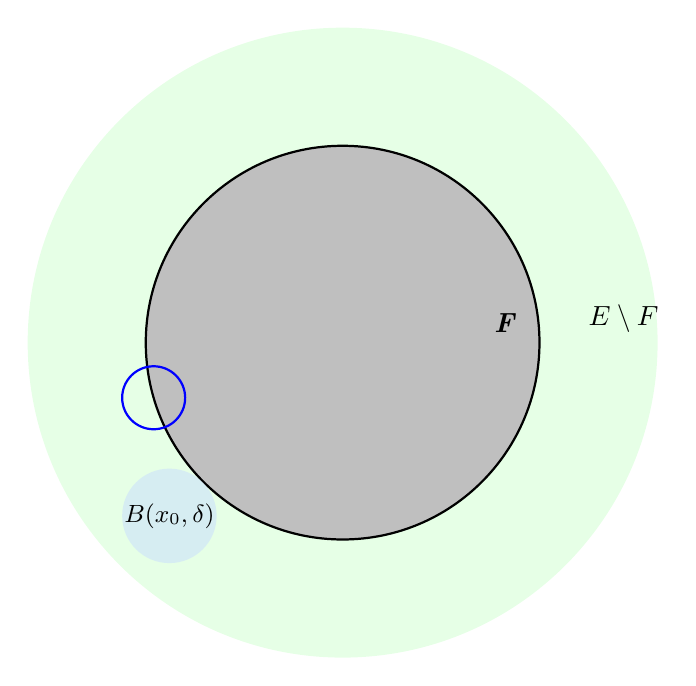
\begin{tikzpicture}
            % Define colors
            \definecolor{lightgreen}{RGB}{230, 255, 230}
            \definecolor{lightblue}{RGB}{200, 220, 255}
            \definecolor{darkgreen}{RGB}{0, 128, 0}

            % Large background circle
            \fill[lightgreen] (0, 0) circle (4cm);

            % Main circle
            \draw[thick, fill=lightgray] (0, 0) circle (2.5cm);
            \node[above right] at (1.8, 0) {\textbf{\textit{F}}};
            \node[above right] at (3, 0) {$E\setminus F$};

            % Small blue circle
            \draw[blue, thick] (-2.4, -.7) circle (0.4cm);

            % Highlighted area for excluded point
            \fill[lightblue, opacity=0.5] (-2.2, -2.2) circle (0.6cm);
            \node (_) at (-2.2, -2.2){\small $B(x_0, \delta)$};
        \end{tikzpicture}
        \caption{Un ensemble fermé\\
            \textit{À la borne, il est impossible de trouver une boules qui appartient à $F$, car il est impossible d'avoir une boule ouverte de  $r = 0$. Exemple: circle bleu foncé}\\
            \textit{Pour tout point dans $E \setminus F$ on peut trouver une boule ouverte}
        }
    \end{subfigure}
    \hfill
    \begin{subfigure}{0.45\textwidth}
        \centering
        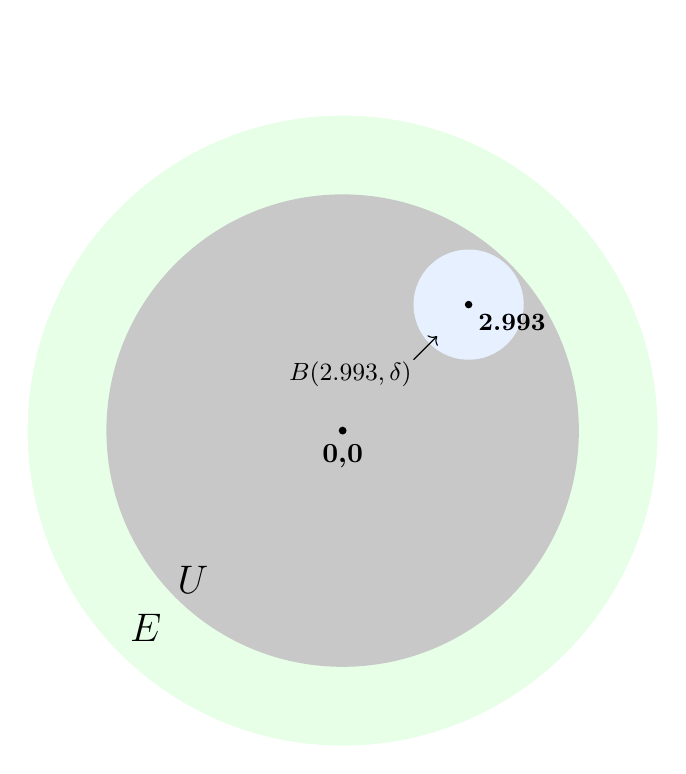
\begin{tikzpicture}
            % Define colors
            \definecolor{lightblue}{RGB}{230, 240, 255}
            \definecolor{lightgray}{RGB}{200, 200, 200}
            \definecolor{darkgreen}{RGB}{0, 128, 0}
            \definecolor{lightgreen}{RGB}{230, 255, 230}

            % Draw large circle
            \fill[lightgreen] (0, 0) circle (4cm);
            \fill[lightgray] (0, 0) circle (3cm);

            % Draw small circle
            \fill[lightblue] (1.6, 1.6) circle (0.7cm);
            \draw[fill=black] (1.6, 1.6) circle(0.4mm);
            \node[below right] at (1.6, 1.6) {\textbf{\small 2.993}};

            \draw[->] (0.9, 0.9)--(1.2, 1.2);
            \node[below left] (_) at (1, 1){\small $B(2.993, \delta)$};
            % Add points and labels
            \node[fill=black, circle, inner sep=1pt, label=below:{\textbf{0,0}}] at (0, 0) {};

            % Add text
            \node[right] at (1, 5) [align=left, text=darkgreen] {
                };
            \node (_) at (-1.9, -1.9){\Large $U$};
            \node (_) at (-2.5, -2.5){\Large $E$};
        \end{tikzpicture} 
        \caption{Un ensemble ouvert\\
            \textit{
                pour tout point pres de la borne
                on peut trouver une boule
                infiniment petite avec des
                points autour ce point inclu dans $U$.
            }
        }

    \end{subfigure}
    \caption{Démonstration des espaces ouverts et fermés}
\end{figure}

\begin{prop}.
    \begin{enumerate}
        \item 
            Une union des ensembles ouverts est aussi ouvert, idem avec l'intersection des ensembles ouverts. 
        \item  
            Une union des ensembles fermé est aussi fermé, idem avec l'intersection des ensembles fermé. 
    \end{enumerate}
\end{prop}

\section{Intérieur, adhérence, frontière}
Soit $A \subset E$. 
\begin{definition}
    Un point $x \in E$ est intérieur à $A$ s'il existe  $\delta > 0$ tel que  $B(x, \delta) \subset A$.\\
    Ensembles des points intérieur à $A$ se note  $Int(A)$ ou  $\mathring{A}$.
\end{definition}
\begin{intuition}
   $Int(A)$ est un ensemble qui est totalement dans  $A$ est se trouve loin des bords. 
\end{intuition}
\begin{tabular}[c]{@{}l@{}r@{}}
    \adjustbox{valign=t}{
    \parbox[t]{0.79\textwidth}{
    \begin{definition}
        Un point $x \in E$ est adhérent à  $A$ si  $\forall r > 0, \, B(x, r) \cap A \neq \O$ (toute boule centré dans $x$ intersecte  $A$).  \\
        Ensemble des points adhérents à $A$ se note  $Adh(A)$ ou  $\overline{A}$.
    \end{definition}
}
}
    &
    \hfill
    \adjustbox{valign=t}{
        \parbox[t]{0.2\textwidth}{
            \vspace{0.3cm}
    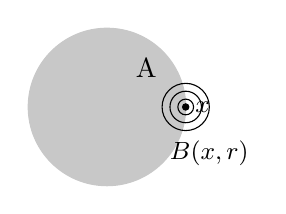
\begin{tikzpicture}
            \definecolor{lightgray}{RGB}{200, 200, 200}
        \filldraw[color=lightgray] (0,0) circle (1cm); 
        \coordinate (x) at (1, 0);
        \filldraw[color=black] (x) circle (0.4mm);
        \node[right] (_) at (x){\small $x$};
        \node (_) at (0.5, 0.5){A};

        \draw (x) circle (0.2cm);
        \draw (x) circle (0.3cm);
        \draw (x) circle (0.1cm);
        \node[below] (_) at (1.3, -0.3){\small $B(x, r)$};
    \end{tikzpicture} 
}
}
\end{tabular}
\begin{intuition}
   Si $A$ est ouvert (ses bords n'appartiennent pas à $A$), ses bords appartiennent à $Adh(A)$. Cette notion est utile pour completer des ensembles.
   \begin{eg}
       $\overline{\Q} = \R$ 
   \end{eg} 
\end{intuition}
\begin{definition}
    $Adh(A) \cap Adh(E \setminus A)$ est le bord de $A$ est s'appelle  la frontière de $A$.
\end{definition}
\section{Suite dans un éspace métrique}
\begin{definition}
    Une suite $(x_n)_{n \in \N}$ converge vers $x \in E$, si  $\forall \epsilon > 0, \exists N \in \N$ tel que :
    \[
    \forall n \ge N, \, d(x_n, x) \le  \epsilon
    \] 
\end{definition}
\begin{prop}
   Soit $A \in E$.\\ 
   \begin{enumerate}
       \item $x \in Adh(A)$ si et seulement si, il existe une suite $(x_n)_{n \in \N}$ d'éléments de $A$ telle que  $x_n \xrightarrow[n \to +\infty]{} x$ 
       \item $A$ est fermé (i.e contient sa frontière) si et seulement si la limite de toute suite  $(x_n)_{n \in \N}$ d'éléments de $A$ appartient à  $A$.
   \end{enumerate}
\end{prop}
\begin{intuition}
   \begin{enumerate}
       \item Si $(x_n)_{n \in \N}$ est d'éléments de  $A$ ($\forall n \in N, \, x_n \in A$), donc elle converge vers un éléments $x$ qui peut être soit dans  $A$, soit la borne des éléments de  $A$, alors à la frontière. 
       \item Si la limite de toute suite $(x_n)_{n \in \N}$ des éléments de  $A$ est aussi dans  $A$, alors la frontière de  $A$ est inclu dans  $A$. Car l'une des suites tend vers la borne.
   \end{enumerate} 
\end{intuition}
\begin{definition}
    Une suite $(x_n)_{x \in \N}$ est de Cauchy si  $\forall \epsilon > 0, \exists N \in \N$ tel que:
    \[
    \forall n, p \ge N, \, d(x_n, x_p) \le \epsilon
    \] 
\end{definition}
\begin{intuition}
   Une suite de Cauchy c'est comme on mesure un point et on le localise, i.e:
   \begin{enumerate}
       \item On dit qu'il est entre $0$ et  $1$.
       \item Ensuite, on precise plus et on dit qu'il est entre  $0.5$ et  $0.6$.
       \item Puis, entre  $0.55$ et  $0.56$
   \end{enumerate}
   On peut infiniment augmenter le niveau de précision. C'est ça l'idée d'une suite de Cauchy.
\end{intuition}
\begin{definition}
    Un éspace métrique $(E, d)$ est \textbf{complet} si toute suite  $(x_n)_{n \in \N}$ d'éléments de  $E$ converge vers une limite  $x$ qui appartient aussi à  $E$.
\end{definition}
\begin{eg}
    Un éspace métrique $(]0, 1], d)$ avec $d$ une distance euclidienne n'est pas complet, car  soit une suite: $x_n = \frac{1}{n}$ dont la limite est $0$. Par contre,  $0 \not\in ]0, 1]$. Donc cet éspace n'est pas complet. 
\end{eg}
\begin{figure}[h]
   \centering 
   \begin{tikzpicture}
       \draw[->] (-1, 0) -- (2, 0); 
       \node[below] (_) at (2,0){$x$};

       \node (_) at (0,0){]};
       \node[below] (_) at (0,-0.3){$0$};
       \node (_) at (1,0){]};
       \node[below] (_) at (1,-0.3){$1$};
       \draw[color=red] (0,0)--(1,0);
   \end{tikzpicture}
   \caption{$(]0, 1], d)$ n'est pas complet}
\end{figure}
\begin{eg}
   Un éspace $(\Q, d)$ n'est pas complet. Car on peut prendre une suite  $x_n$ tendant vers  $\sqrt{2} \not\in \Q$.
\end{eg}

\begin{figure}[H]
    \centering
    \incfig{q_not_complete}
    \caption{$\Q$ pas complet}
    \label{fig:q_not_complete}
\end{figure}

\begin{definition}
    Soit une suite $(x_n)_{n \in \N}$ et une application  $\phi:\N \to \N$ \underline{strictement croissante}. Une suite $(x_n)_{\phi(n)}$ est appellée une sous-suite.
\end{definition}
\begin{eg}
    Soit une application $\phi: \N \to \N$ telle que $\phi(n) = 2n$. Donc  $(x_n)_{\phi(n)}$ est une sous-suite de  $(x_n)_{n \in \N}$ et:
    \[
        (x_n)_{\phi(n)} = \{x_0, x_2, x_4, \ldots\}
    \] 
\end{eg}

\section{Compacité}
\begin{definition}
    Soit $F \subset E$. Un \textbf{recouvrement ouvert} de $F$, est une union des enesembles ouverts:  $\bigcup_{i \in I} U_i$ tel que $F \subset \bigcup_{i \in I} U_i$
\end{definition}
\begin{eg}
    Soit $F = ]0, 1[$. Soit $A = \left\{]\frac{1}{n}, 1 + \frac{1}{n}[, n \in N\right\}$. $F \subset \bigcup_{n \in N^{*}} A_n$ i.e union infinie des $A_i$ couvre $F$.
\end{eg}
\begin{definition}
    Un ensemble $F \subset E$ est \textbf{compact} si \underline{pour tout} recouvrement ouvert, i.e \underline{pour tout} union des ensembles ouvert $\bigcup_{i \in I} U_i$ qui couvre $F$, on peut prendre un nombre \underline{fini} des  $U_i$ et couvrir $F$.
\end{definition}
\begin{theorem}
    Un ensemble $K \subset E$ est compact, si toute suite $(x_n)_{n \in \N}$ des éléments de $K$, possede une sous-suite qui converge  vers un éléments $x \in K$.
\end{theorem}
\begin{intuition}
    S'il existe tel suite $(x_n)_{n \in \N}$ sans sous-suite convergente vers un éléments de  $K$, donc les valeurs sont en-dehors de  $K$ et donc il existe un ensemble qui couvre $K$  seulement avec un nombre infini des ensembles. 
\end{intuition}
Pourquoi a-t-on besoin de compacité? Car cela nous donne une
\begin{prop}
    Si $K \subset E$ est compact, alors $K$ est fermé et borné.\\
    Si $K$ est compact est  $F$ est borné, donc  $K \cap F$ est compact\\
    Si $K$ est compact, donc  $K$ est complet
\end{prop}
\begin{property}
    La différence entre \textit{compacité} et {complecité}:
    \begin{itemize}
        \item complecité nous assure qu'il n'y a pas de trou dans un espace
        \item compacité nous assure qu'un ensemble est fermé et borné
    \end{itemize}
\end{property}
\section{Limites et applications continues}
2



\nocite{*}
\printbibliography


\end{document}

